\documentclass[12pt, a4paper, titlepage, twoside]{article}
\usepackage[margin=1.2cm,inner=2.5cm,outer=1.5cm,bottom=2cm]{geometry}
\usepackage{amsmath}
\usepackage{amsfonts}
\usepackage{bm}
\usepackage{fixmath}
\usepackage{mathtools}
\usepackage{amssymb}
\usepackage{amsthm}
\usepackage{tikz}
\usepackage{pgfplots}
\usepackage{graphicx}
\usepackage{adjustbox}
\usepackage{multicol}
\usepackage{hyperref}
\usepackage{wrapfig}
\usepackage{caption}
\usepackage{float}
\usepackage{enumitem}
\usepackage{tkz-euclide}
\usepackage{siunitx}
\usepackage{longtable}
\usepackage{makecell}
\usepackage{newunicodechar}
\usepackage{kpfonts,baskervald}
\usepackage{hhline}

\newunicodechar{¥}{\textyen}
\DeclareTextCommandDefault{\textyen}{%
  \vphantom{Y}%
  {\ooalign{Y\cr\hidewidth\yenbars\hidewidth\cr}}%
}

\newcommand{\yenbars}{%
  \vbox{
     \hrule height.1ex width.4em
     \kern.15ex
     \hrule height.1ex width.4em
     \kern.3ex
  }%
}


\usepackage[many]{tcolorbox}

\graphicspath{{res/}}
\newcommand*{\im}{\mathbold{i}}
\newcommand*{\N}{\mathbb{N}}
\newcommand*{\Z}{\mathbb{Z}}
\newcommand*{\Q}{\mathbb{Q}}
\newcommand*{\I}{\mathbb{I}}
\newcommand*{\R}{\mathbb{R}}
\newcommand*{\C}{\mathbb{C}}
\newcommand*{\e}{\textrm{e}}
\linespread{1.5}

\renewcommand{\qedsymbol}{$\blacksquare$}

\newtheorem*{theorem*}{Theorem}

\hypersetup{
    colorlinks,
    citecolor=blue,
    filecolor=blue,
    linkcolor=blue,
    urlcolor=blue
}

\newtcolorbox{kp}[1][]{%
    enhanced,breakable,title=\textbf{#1},
    segmentation style={solid, violet!30, line width=1pt},
    colframe = red!25,
  	colback  = red!10,
  	coltitle = red!20!black
}

\newcounter{excount}[subsection]

\newtcolorbox{ex}{%
    enhanced,breakable,title=\textbf{Worked example \thesubsection.\arabic{excount}},
    segmentation style={solid, black, line width=1pt}
}

\newtcolorbox{pf}[1][]{%
    enhanced,breakable,title=#1,
    segmentation style={solid, blue!30, line width=1pt},
    colframe = blue!25,
  	colback  = blue!10
}

\newtcolorbox{fr}[1][]{%
    enhanced,breakable,title=\textbf{Further reading: #1},
    segmentation style={solid, violet!30, line width=1pt},
    colframe = violet!25,
  	colback  = violet!10,
  	coltitle = violet!20!black
}

\newcommand\crule[1][black]{\textcolor{#1}{\rule{0.5cm}{0.5cm}}}


\newtcbox{\inlinebox}[2][]{enhanced,
 box align=base,
 nobeforeafter,
 colback=#2,
 colframe=#2,
 size=small,
 left=0pt,
 right=0pt,
 boxsep=2pt,
 #1}

\setcounter{section}{-1}
\setcounter{tocdepth}{2}
\pgfplotsset{compat=1.11}

\begin{document}
	\begin{titlepage}
  	\null\vfill

  	\begin{center}
  		{\Huge IB Mathematics Analysis and Approaches} \vskip 2cm
  		{\Large A Formal Approach} \vskip 1cm
 	\end{center}

	\vfill
	\vfill
	
	\begin{center}
  		{\Large Liam McQuay}
 	\end{center}

	\end{titlepage}

	\newpage
	
	\tableofcontents
	
	\newpage
	
\section{About the course companion}

	\subsection*{Overview}

	\paragraph{}
	This textbook covers all of IB Mathematics Analysis and Approaches at both SL and HL. This 
	is \textbf{not} your typical textbook. Most textbooks will teach the content with many concrete examples and explain
	things in quite a bit of detail. I deem some of this detail as unnecessary and as content which a student can figure out
	for themself. This book with be more abstract and formal; it won't go through many examples and won't provide as many
	trivial exercises as other textbooks do. 
	The book also includes extra material outside the syllabus to enhance your learning (and provide further context for 	
	syllabus content when needed). Extra content will be clearly indicated so you know what is and isn't in the syllabus. However, I highly 
	recommend going through all the extra content anyway. That being said, this textbook is recommended to those who have a great
	interest in mathematics and would like to learn more than just what the course teaches them. If you find that your mathematics 
	ability is quite weak (for example, level 5 or below), this may not be the textbook for you.

	\paragraph{}
	As the title of the book says, it approaches the content formally. It will contain mathematical proofs for some of the 
	major theorems to provide you both reasoning for what you learn as well as an idea of what formal proofs look like in University 
	mathematics and beyond. From my personal experience learning mathematics, I found most textbooks were only somewhat helpful and 
	didn't fully explain concepts the best way. I am aware of how most students understand mathematics and will do my best to present the 
	content as such. 

	\paragraph{}
	The Analysis and Approaches (AA) content is covered for both SL and HL students. Throughout the book,
	I have indicated whether content is HL content (and labelled such sections \textbf{HL}). If a section doesn't have
	any indication of this kind, it will be SL content too and you'll need to know it. 
	Note that the textbook will be in an order in which you can follow linearly from start to finish. This ensures all (or most) prerequisites are 
	covered before you move on to the next topic.
	
	\paragraph{}
	Moreover, there will be sections labelled \textbf{FC} for \textbf{Further Content}. This will typically be out-of-syllabus topics which may
	be useful. I've done this because unfortunately I'm not very happy with the lack of rigor provided in the AA course (and I certainly feel the 
	same way about the AI course too). I recommend you look into this content to further your learning about mathematics. If you do want to
	skip it however, you can.

	\subsection*{Key Points}
	
	\paragraph{}
	Any key points (formulas, equations, identities or equivalent) which need to be displayed for clarity shall be displayed like so:\\
	
	\begin{kp}[Euler's identity]
		$$\e^{\im \pi} + 1 = 0$$
	\end{kp}

	\subsection*{Worked Examples}

	\paragraph{}
	The book will have a number of worked examples per chapter which span the types of short-answer questions you may get in an 
	examination and how a candidate can respond to such questions. Worked examples look like this:\\
	
	
	\begin{ex}
		\hfill \\
		An arithmetic sequence $\{u_n\}$ has first three terms: $u_1 = 1, u_2 = 5,$ \\ $u_3 = 9$.\\
		
		\textbf{(a)} Write down the common difference
		
		\textbf{(b)} Hence find $u_8$\\
		
		\tcbline
		
		\hfill \\
		\textbf{(a)} The common difference, $d$, is obtained by subtracting one term from the previous:\\
		$d = u_3 - u_2 = 9 - 5 = 4$ or equivalently $d = u_2 - u_1 = 5 - 1 = 4$\\
		
		\textbf{(b)} Using the fact that $u_n = u_1 + d(n-1)$, we can simply substitute the values of $d$ and $n$:\\
		$u_8 = 1 + 4(8-1) = 1 + 4 \cdot 7 = 1 + 28 = 29$
		
	\end{ex}
	
	\paragraph{}
	You are encouraged to find other methods of answering these questions (if any) in order to determine and use the methods 
	which are best for you.
	
	\subsection*{Proofs}
	
	\paragraph{}
	As stated, this book will contain mathematical proofs for most of the major theorems encountered in the course. Most of these
	you will not need to know. However, you are encouraged to read these proofs as they will help you better understand the content
	you are learning. It's one thing having formulas given to you in a booklet where you know how and when to use them, but another
	if you don't \textbf{understand} them. Proofs look like this:\\
	
	\begin{pf}
		\label{pf:root2}
		\begin{theorem*}
			$\sqrt{2}$ is irrational
		\end{theorem*}

		\tcbline		
		
		\begin{proof}
			Suppose $\sqrt{2}$ \textbf{is} rational (i.e. $\sqrt{2} \in \Q$).\\
			
			Then there exist $m, n \in \Z$ such that $\sqrt{2} =  \dfrac{m}{n}$ is irreducible (i.e. $\gcd(m,n) = 1$), 
			as per the definition of a rational number. \\
			
			Squaring both sides yields: $2 = \dfrac{m^2}{n^2}$, which implies $m^2 = 2n^2$. \hfill \textbf{(1)} \\
			
			This means $m^2$ is even and thus that $m$ must be even (since an odd number squared is odd).\\
			
			$m$ can hence be expressed as $2k_1$ for some $k_1 \in \Z$. Putting $m$ back into equation \textbf{(1)} yields:\\
			
			$(2k_1)^2 = 2n^2 \implies 4{k_1}^2 = 2n^2 \implies n^2 = 2{k_1}^2$, which means $n^2$ must be even and hence $n$
			must be even.\\
			
			Thus $n$ can be expressed as $2k_2$ for some $k_2 \in \Z$.\\
			
			Now $m = 2k_1$ and $n = 2k_2$ and hence, $\sqrt{2} = \dfrac{2k_1}{2k_2}$, which is clearly reducible by canceling
			the $2$s from the numerator and denominator, implying $\dfrac{m}{n}$ is reducible.\\
			
			This is a contradiction to the definition of rational numbers, as an irreducible fraction can't be found. Hence,
			$\sqrt{2}$ is irrational.
		\end{proof}
		
	\end{pf}
	
	\paragraph{}
	Notice the $\blacksquare$ symbol at the bottom-right corner. This symbol means \textit{Quod Erat Demonstrandum} 
	(Latin for ``what was to be shown''). Mathematicians use this as a way of telling a reader that their proof is finished.
	If you need to give a proof for an examination, you can put this at the end of your response as a formality, but this isn't
	required.
	
	\subsection*{Exercises}
	
	\paragraph{}
	Most textbooks include drill exercises at the end of each chapter. This book will have a limited number of drill exercises at the end of
	each chapter section and exam-style questions and/or word problems as exercises at the end of each chapter. Each exercise will have 
	a difficulty level indicated:\\
	
	\crule[green] = Easy \quad \crule[yellow] = Medium \quad \crule[red] = Hard \quad \crule[gray!30] = Out of syllabus

	\paragraph{}
	The out of syllabus questions will naturally be more challenging. However, you are advised to attempt them to the best of your
	ability.
	
	\subsection*{Further Reading}
	
	\paragraph{}
	You will also find boxes with further information outside the syllabus about the content of the book. This may discuss history, 
	some interesting mathematical fact(s) or something else. You are \textbf{not} expected to know them for the exams. These will look 
	like this:\\
	
	
	\begin{fr}[Peano's axioms]
		\label{fr:peano}
		An \textbf{axiom} in mathematics is a statement which we assume to be true (without proof) so we can use it as a basis for further
		arguments made. An example includes \textit{Peano's Axioms} (by mathematician \textit{Giuseppe Peano}), which define 
		the set of natural numbers $\N$. Define $0$ to be unity. Define a \textit{successor} function $S(n)$ such that $1 = S(0), 
		2 = S(1) = S(S(0), ..$.\\
		
		Then Peano's Axioms are:
		
		\begin{enumerate}
			\item $0$ is a natural number*
			\item For any natural number $n$, $S(n)$ is also a natural number
			\item If $m$ and $n$ are natural numbers such that $m=n$, then $S(m) = S(n)$
			\item There is no such natural number $n$ for which $S(n) = 0$*
			\item If $K$ is a subset of $\N$ which contains $0$ and the successor of every number in $K$, then
			$K=\N$ (induction axiom)*
		\end{enumerate}
		
		* - Note that some start the natural numbers at $1$. If so, one can simply define $1$ to be unity and make the
		necessary amendments to the axioms.\\
		
		The axioms above define the nature of natural numbers and are a basis for arithmetic in $\N$. For any math
		we do, we have justification for our steps and justification for our justification. However, if we keep trying to
		find justification for anything, there has to be a point where we must stop; we encounter statements which have
		no justification. If these unjustifiable statements break down (somehow), all of math would break down.
	\end{fr}
	
	\subsection*{Calculators}
	
	\paragraph{}
	Due to overlap with the two courses, this textbook will \textbf{not} indicate questions when a calculator (GDC) is disallowed.
	Generally, calculator use is allowed for any question in the textbook, but I advise you to try questions without a calculator first and use 
	it if it seems appropriate.
	
	\newpage
	
\section{Preliminaries}	

	\paragraph{}
	This chapter recaps some information on symbols, numbers and approximations which you may or may not be familiar with.
	You should also be aware of the constants $\pi$ and $\e$ and be able to find and use them on your calculator. This chapter
	also looks at counting principles for HL students.
	
	\subsection{Symbols}
	
	\paragraph{}
	The list of symbols used in this book and the IB is given below. This does \textbf{not} cover everything; only symbols
	which you must be familiar with before learning the course. You can find the full notation list in the course guide.
	
	{\centering \subsubsection*{Set symbols}}
	
		{\centering
		\begin{longtable}{|c|c|c|} 
 			\hline
			\textbf{Symbol} & \textbf{Meaning} & \textbf{Example (if applicable)}\\
			\hhline{|=|=|=|}
			$\N$ & The set of natural numbers & -\\
			\hline
			$\Z$ & The set of integers & -\\
			\hline
			$\Z^+$ & The set of positive integers & -\\
			\hline
			$\Z^-$ & The set of negative integers & -\\
			\hline
			$\Q$ & The set of rational numbers & -\\
			\hline
			$\Q^+$ & The set of positive rational numbers & -\\
			\hline
			$\Q^-$ & The set of negative rational numbers & -\\
			\hline
			$\R$ & The set of real numbers & -\\
			\hline
			$\R^+$ & The set of positive real numbers & -\\
			\hline
			$\R^-$ & The set of negative real numbers & -\\
			\hline
			$\C$ & The set of complex numbers & -\\
			\hline
			$\varnothing$ & The empty set & -\\
			\hline
			$U$ & The universal set & -\\
			\hline
			$\{x \mid ...\}$ & Set of all elements $x$ for which $...$ & $\{x \mid x \geqslant 5\}$\\
			\hline
			$\in$ & Element of & $-5 \in \Z$\\
			\hline
			$\not\in$ & Not an element of & $-5 \not\in \N$\\
			\hline
			$n(A)$ & Number of elements in $A$ & -\\
			\hline
			$\cap$ & Intersection of sets & $A \cap B$\\
			\hline
			$\cup$ & Union of sets & $A \cup B$\\
			\hline
			$A'$ & \makecell{Complement of $A$ (set of all elements \\ \textbf{not} in $A$)} & -\\
			\hline
			$\subset$ & Proper subset of & $A \subset B$\\
			\hline
			$\subseteq$ & Subset of or equal to & $A \subseteq B$\\
			\hline
			$\not\subset$ & Not a subset of & $A \not\subset B$\\
			\hline
			$\not\subseteq$ & Not a subset of or equal to & $A \not\subseteq B$\\
			\hline
			$[a,b]$ & \makecell{The closed interval of values between\\ $a$ and $b$ inclusive} & $x \in [a,b]$\\
			\hline
			$(a,b)$ & \makecell{The open interval of values between\\ $a$ and $b$ non-inclusive} & $y \in (a,b)$\\
			\hline
		\end{longtable}}
	
	{\centering \subsubsection*{Relation symbols}}
	
	{\centering
		\begin{longtable}{|c|c|c|} 
 			\hline
			\textbf{Symbol} & \textbf{Meaning} & \textbf{Example (if applicable)}\\
			\hhline{|=|=|=|}
			$=$ & Equal & $a=b$\\
			\hline
			$\neq$ & Not equal & $a \neq b$\\
			\hline
			$\equiv$ & Identical & $a \equiv b$\\
			\hline
			$\approx$ & Approximately equal to & $a \approx b$\\
			\hline
			$>$ & Greater than & $a > b$\\
			\hline
			$\geqslant$ & Greater than or equal to & $a \geqslant b$\\
			\hline
			$<$ & Less than & $a < b$\\
			\hline
			$\leqslant$ & Less than or equal to & $a \leqslant b$\\
			\hline
		\end{longtable}}
	
	{\centering \subsubsection*{Function symbols}}
	
	{\centering
		\begin{longtable}{|c|c|c|} 
 			\hline
			\textbf{Symbol} & \textbf{Meaning} & \textbf{Example (if applicable)}\\
			\hhline{|=|=|=|}
			$f : A \to B$ & \makecell{The function $f$ maps\\ the set $A$ to the set $B$} & $f : \R \to \R^+$\\
			\hline
			$f : x \mapsto y$ & \makecell{The function $f$ maps\\ the element $x$ to the element $y$} & $f : x \mapsto e^x$\\
			\hline
			$f(x)$ & The function $f$ of element $x$ & $f(x) = e^x$\\
			\hline
			$f^{-1}(x)$ & The inverse function of $f$ & $f^{-1}(x) = \ln(x)$\\
			\hline
			$f \circ g(x)$ & The composite function of $f$ and $g$ & $f \circ g(x) = e^{g(x)}$\\
			\hline
		\end{longtable}}
	
	\newpage	
	
	{\centering \subsubsection*{Geometry symbols}}
	
	{\centering
		\begin{longtable}{|c|c|c|} 
 			\hline
			\textbf{Symbol} & \textbf{Meaning} & \textbf{Example (if applicable)}\\
			\hhline{|=|=|=|}
			$P(x,y)$ & The point with coordinates $(x,y)$ & $P(1,2)$\\
			\hline
			$[AB]$ & The line segment with endpoints $A$ and $B$ & -\\
			\hline
			$AB$ & The length of the segment $[AB]$ & $AB = 5$\\
			\hline
			$(AB)$ & The line containing the points $A$ and $B$ & -\\
			\hline
			$\hat{A}$ & The angle of point $A$ & $\hat{A} = \ang{45}$\\
			\hline
			$A\hat{B}C$ & The angle between segments $[AB]$ and $[BC]$ & $A\hat{B}C = \ang{30}$\\
			\hline
			$\Delta ABC$ & The triangle with vertices $A,B$ and $C$ & -\\
			\hline
		\end{longtable}}
	
	\hfill
	
	\subsection{Number systems}
	
	\paragraph{}
	A number system refers to a set of numbers which have a certain property. The Venn diagram below shows common number systems 
	looked at in the IB course.
	
	\begin{figure}[H]
		\centering
		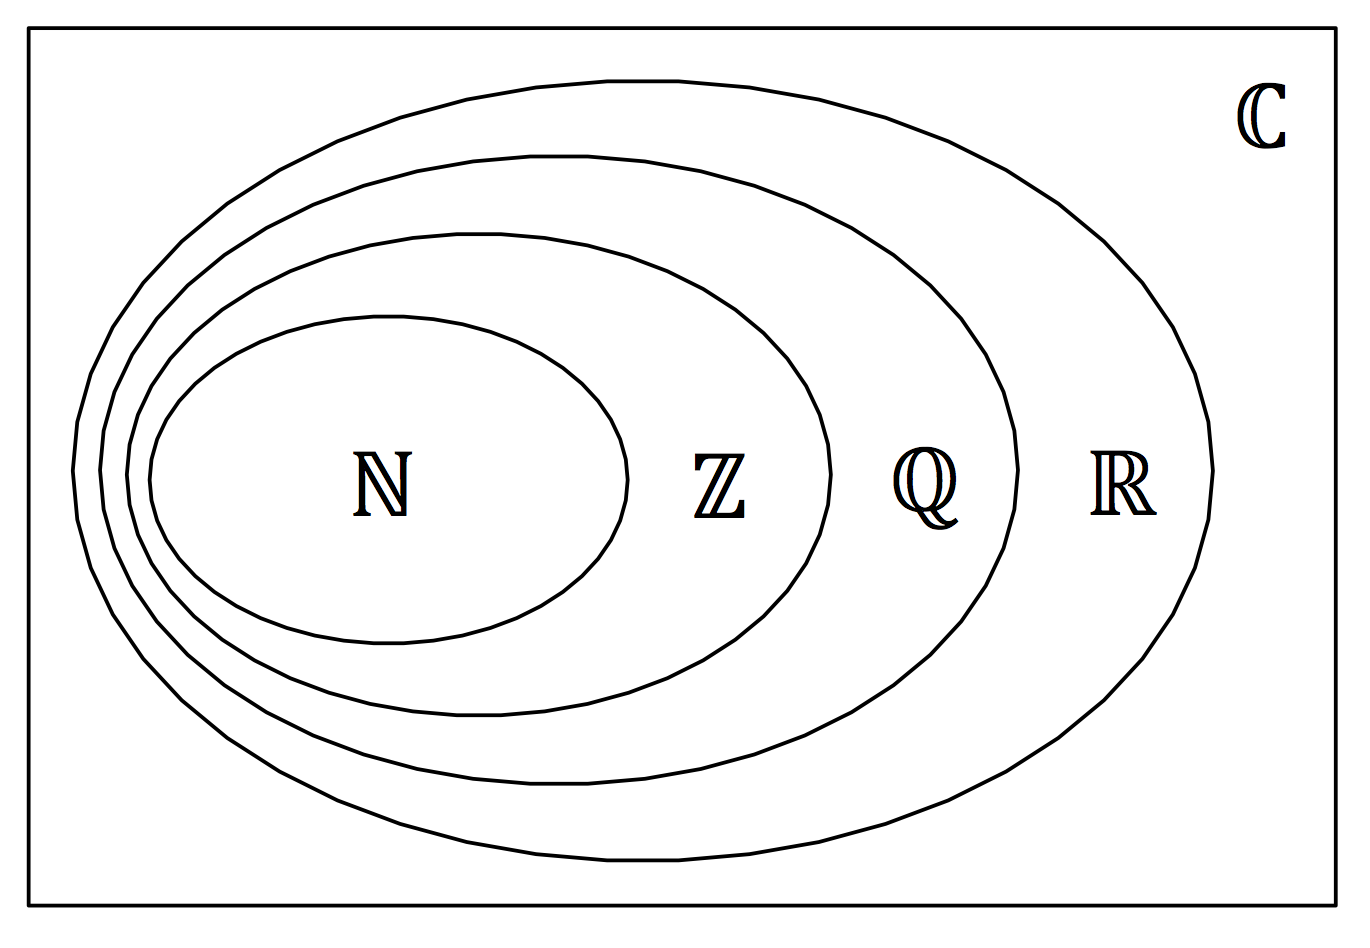
\includegraphics[width=12cm]{algebra-venn.png}
		\caption*{\textbf{Some common number systems and their set relations}}
	\end{figure}
	
	\paragraph{}
	$\N$ is the set of \textit{natural numbers}: $\N = \{0,1,2,3,...\}$ (sometimes $0$ is excluded). These are numbers which we can 
	``count	naturally'' (such as the number of books on a bookshelf). $\N$ holds some importance in mathematics (see 
	\textbf{Peano's axioms} on page \pageref*{fr:peano} and \textbf{Countability} on page \pageref*{fr:countability}).
	
	\paragraph{}
	$\Z$ is the set of \textit{integers}: $\{..., -3, -2, -1, 0, 1, 2, 3, ...\}$. These are numbers which are formed by taking $\N$ and adding
	0 (if not already in $\N$) and $-\N$, which are \textit{negative} natural numbers. Integers hold importance in topics such as
	discrete mathematics. Note that the natural numbers are contained in the integers, so we say $\N \subset \Z$, which is read as
	``$\N$ is a subset of $\Z$''.
	
	\paragraph{}
	$\Q$ is the set of \textit{rational numbers}: $\{\frac{m}{n} : m,n \in \Z, n \neq 0\}$. This is the set of all numbers which can be
	expressed as fractions, such as $\frac{1}{2}$ or $\frac{4}{5}$. The rationals are what we describe as \textit{dense}. This means
	between any two rationals $p$ and $q$ where $p < q$, we can find another rational $r$ for which $p < r < q$. Despite this, we can
	still count the rationals like we can count the natural numbers or the integers (see \textbf{Countability} on page 
	\pageref*{fr:countability}). We also have that $\Z \subset \Q$, because we can express any integer $a$ as a fraction: $\frac{a}{1}$.
	
	\paragraph{}
	$\R$ is the set of \textit{real numbers}. This is the set of all numbers on the number line, including numbers which are \textbf{not}
	rational (which we say are \textit{irrational}). Think of the real numbers as the rational numbers with the ``gaps filled'' or the set of
	all possible decimal numbers. Some examples of irrational numbers are $\sqrt{2} = 1.4142135624...$ and $\pi = 3.1415926536...$, 
	neither of which can be expressed as fractions (the proof of $\sqrt{2}$ being irrational is on page \pageref*{pf:root2}). In fact, a real
	number is rational if and only if it has a terminating digit or repeating decimal digits. We clearly have that $\Q \subset \R$.
	
	\paragraph{}
	$\C$ is the set of \textit{complex numbers}. This is the set of all numbers of the form $a + b\im$, where $a,b \in \R$ and $\im$ is an 
	\textit{imaginary} number defined as $\sqrt{-1}$. The complex numbers serve a purpose in finding roots of polynomials. It can be proven
	that every polynomial of degree $n$ with complex coefficients has exactly $n$ complex roots (some of which may be repeated).
	They are also looked at further in Complex Analysis at university. Complex numbers are covered at HL, so SL students don't 
	need to know this.
	
	\hfill
	
	\begin{fr}[Countability]
		\label{fr:countability}
		As stated, the natural numbers $\N$ are numbers which we can count with. Therefore, we can use these to determine whether
		other sets are countable. What we mean by countable is that we can count each element in an \textit{infinite} set one at a time; 
		even though it would take us forever! Some definitions may say a finite set is countable; there's no problem with this. However this
		text will take countable to exclude the finite case so as to use ``countable'' to mean countably-infinite sets distinct from finite sets,
		avoiding ambiguity.\\
		
		The formal definition for a set $Y$ to be countable (countably-infinite) is that there exists a \textbf{bijection} from $\N$ to $Y$. That is, we
		can find a function $f: \N \to Y$ such that $f$ is both \textbf{injective} (one-to-one) and \textbf{surjective} (onto). The definitions of
		these are given below:
		
		\begin{itemize}
			\item A function $f : X \to Y$ is \textit{injective} when for $x_1, x_2 \in X$, we have that $f(x_1) = f(x_2)$ implies $x_1 = x_2$.
			\item A function $f : X \to Y$ is \textit{surjective} when for all $y \in Y$, we can find some $x \in X$ for which $f(x) = y$.
		\end{itemize}
		
		We can now use these definitions to show that some familiar sets are countable (please be aware though that there is no need
		to be able to do this at IB, no matter what level you're taking):\\
	\end{fr}
	
	\hfill
	
	\begin{pf}
		\label{pf:z-count}
		\begin{theorem*}
			$\Z$ is countable
		\end{theorem*}

		\tcbline		
		
		\begin{proof}
			\textit{Note: in this proof, $\N$ starts at $0$}\\
			
			We must find a function $f: \N \to \Z$ such that $f$ is bijective (injective and surjective).\\
			
			Consider $f(n) = 
			\begin{cases} 
				\dfrac{n}{2}, & n \text{ is even}\\
				-\dfrac{n+1}{2}, & n \text{ is odd}\\
			\end{cases}$\\
			
			\textbf{Injection:} suppose $f(m) = f(n)$. Then either:\\ 
			
			$\dfrac{m}{2} = \dfrac{n}{2}$ \hfill \textbf{(1)}\\ 
			
			or $-\dfrac{m+1}{2} = \dfrac{n}{2}$ \hfill \textbf{(2)}\\
			
			(without loss of generality).\\
			
			For \textbf{(1)}, it is clear that $m=n$ as required.\\
			For \textbf{(2)}, $-m-1 = n \implies m+n = -1$, which is not possible in $\N$.\\
			
			Hence, $f$ must be injective.\\
			
			\textbf{Surjection:} let $z \in \Z$; we must show there is an $n \in \N$ for which $z = f(n)$\\
			
			Let $z \geq 0$ ($z$ is positive or 0) and consider $n = 2z$. Then $f(n) = f(2z) = \dfrac{2z}{2} = z$\\
			
			Now let $z < 0$ ($z$ is negative) and consider $n = -2z-1$ ($n$ is odd). Then $f(n) = f(-2z-1) = -\dfrac{-2z}{2} = z$\\
			
			We have found values of $n$ for which any $z \in \Z$ can be produced. Hence, $f$ is surjective.\\
			
			Since $f$ is injective and surjective, it is bijective. Hence a bijection between $\N$ and $\Z$ exists, which means
			$\Z$ is countable. 
		\end{proof}
	\end{pf}
	
	\begin{pf}
		\label{pf:q-count}
		\begin{theorem*}
			$\Q$ is countable
		\end{theorem*}

		\tcbline		
		
		\begin{proof}
			Since we have established that $\Z$ is countable, we can use this property to prove $\Q$ is.\\
			
			Consider the set $S_n = \left\lbrace \dfrac{m}{n} \mid m \in \Z \right\rbrace$ for $n \in \Z^+$.\\
			
			It is clear that $\displaystyle \Q = \mathop{\bigcup}_{n=1}^{\infty} S_n = S_1 \cup S_2 \cup S_3 \cup ...$\\
			
			$S_n = \dfrac{1}{n} \{m \mid m \in \Z\} = \dfrac{1}{n} \Z$. Since $\Z$ is countable and we are simply multiplying
			each term of $\Z$ by a constant, so $S_n$ must be countable.\\
			
			We will use the fact (without proof) that the countable union of countable sets is countable. This proves that $\displaystyle 
			\mathop{\bigcup}_{n=1}^{\infty} S_n$ is countable and hence that $\Q$ is countable.
		\end{proof}
		\hfill
		
		Note that if you aren't happy with the proof using the fact that the countable union of countable sets is countable,
		I've included a proof of this fact in \textbf{Appendix A} on page \pageref*{apA:ctble-union}. Note also that
		there are other ways to prove $\Q$ is countable; one is written in \textbf{Appendix A} on page \pageref*{apA:q-count-fta} which
		uses (and proves!) the \textit{Fundamental Theorem of Arithmetic} instead (\textbf{Appendix A}, page \pageref*{apA:fta}). We can also
		prove that $\R$ is \textbf{un}countable (\textbf{Appendix A}, page \pageref*{apA:r-uncount}).
	\end{pf}
	
	\subsection{Approximations}
	
	\paragraph{}
	While this topic is officially covered in the AI course, it may be worth looking into anyway (as an AA student).
	
	\paragraph{}
	In mathematics, we may find values which have a large number of trailing decimal digits, some of which may not even terminate
	(such as irrational numbers). It may come handy to express such numbers either in \textit{exact form} (if possible) or in 
	\textit{approximated form}.\\
	
	\begin{kp}[Exact form]
		A number is in exact form if it is written such that there is complete certainty (that is, the expression provides all information
		about that number). Some examples are:
		
		\begin{longtable}{|c|c|}
			\hline
			\textbf{Number in exact form} & \textbf{Number not in exact form}\\
			\hhline{|=|=|}
			$\sqrt{2}$ & $1.414213562$\\
			\hline
			$\pi$ & $3.141592654$\\
			\hline
			$\e$ & $2.718281828$\\
			\hline
		\end{longtable}
	\end{kp}
	
	\paragraph{}
	A number in approximated form is usually written as a decimal number with a terminating digit, but can also be written as a fraction.
	For example, $3.14$ is an approximation of $\pi$ and so is $\dfrac{22}{7} = 3.\overline{142857}$ (note that a horizontal bar over the
	decimal digits indicates that the group of digits is recurring). We say that $\pi \approx 3.14$ and $\pi \approx \dfrac{22}{7}$.
	
	\paragraph{}
	When approximating, we usually provide the \textit{degree} of an approximation; how close it is to the exact value. The course looks 
	at two of these: \textit{decimal places} and \textit{significant figures}.
	
	\paragraph{}
	Decimal places are the number of decimal digits which are written in the approximated form (the number of digits which come after
	the whole part). For example, $3.1416$ is correct to $4$ decimal places (4 d.p.) while $103.4$ is correct to 1 d.p.
	
	\paragraph{}
	Note that when rounding to a number of decimal places, the last digit to be written ($d_n$) must be rounded up if the 
	digit to the right of $d_n$ ($d_{n+1}$) is greater than or equal to 5. Also, $d_{n+1}$ must \textbf{not} be rounded.\\
	
	\begin{kp}[Decimal places]
		A number in approximated form given correct to $n$ decimal places has $n$ decimal digits provided. Some
		approximations of $\sqrt{2}$ are given below:
		
		\begin{longtable}{|c|c|}
			\hline
			\textbf{Approximation} & \textbf{Decimal places}\\
			\hhline{|=|=|}
			$1$ & $0$\\
			\hline
			$1.4$ & $1$\\
			\hline
			$1.41$ & $2$\\
			\hline
			$1.414214$ & $6$\\
			\hline
			$1.4142136$ & $7$\\
			\hline
			$1.41421356$ & $8$\\
			\hline
		\end{longtable}
	\end{kp}
	
	\paragraph{}
	Significant figures are the digits which ``have meaning'' to the approximation. Note that these don't necessarily include
	only the decimal digits; this applies to all digits of a number. Significant figures have a few rules associated with them.\\

	\begin{kp}[Significant figures]
		\begin{itemize}
			\item Any non-zero digit is significant
			\item Any zeros between two significant zeros are significant
			\item Trailing zeros are significant \textbf{only} when they are in the decimal part of a number
		\end{itemize}
		
		Additionally, the rounding rule described with decimal places applies here as well. Some approximations of 
		$1006.50089$ are given below:
		
		\begin{longtable}{|c|c|}
			\hline
			\textbf{Approximation} & \textbf{Significant figures}\\
			\hhline{|=|=|}
			$1000$ & $1$\\
			\hline
			$1000$ & $2$\\
			\hline
			$1010$ & $3$\\
			\hline
			$1007$ & $4$\\
			\hline
			$1006.5$ & $5$\\
			\hline
			$1006.50$ & $6$\\
			\hline
			$1006.501$ & $7$\\
			\hline
			$1006.5009$ & $8$\\
			\hline
			$1006.50089$ & $9$\\
			\hline
			$1006.500890$ & $10$\\
			\hline
			$1006.5008900$ & $11$\\
			\hline
		\end{longtable}
	\end{kp}	
	
	\paragraph{}
	It is also worth knowing how to express numbers in \textit{standard form}:\\
	
	\begin{kp}[Standard form]
		A number is in standard form if it is expressed as $a \times 10^k$, where \\ $1 \leq a < 10$ and $k \in \Z$.
	\end{kp}
	
	\paragraph{}
	For example, $0.0000456$ is expressed as $4.56 \times 10^{-5}$ and $12300000$ is expressed as $1.23 \times 10^{7}$.
	
	\paragraph{}
	Another property to consider is the \textit{upper and lower bounds} of an approximation. When a number is rounded,
	these bounds describe the \textbf{range} of possible values for the exact value. For instance, suppose $a \approx 4.23$ approximated
	to 2 d.p. Then the range of values of $a$ is: $4.225 \leq a < 4.235$. Note that the last part is given a strict inequality.
	This is because $a$ can't be $4.235$ exactly (otherwise it would've been rounded to $4.24$), but it can still be anything less
	than that (such as $4.2349999$). \\
	
	\begin{kp}[Upper and lower bounds]
		Given an approximation of a value, one can find the upper and lower bounds of the exact number by considering the range of possible
		values which produce the approximation when rounded. Some examples are given below:\\
		
		\begin{longtable}{|c|c|c|}
			\hline
			\textbf{Approximation} & \textbf{d.p. / s.f.} & \textbf{Range of values}\\
			\hhline{|=|=|=|}
			$1.41$ & 2 d.p. & $1.405 \leq x < 1.415$\\
			\hline
			$56.789$ & 3 d.p. & $56.7885 \leq x < 56.7895$\\
			\hline
			$1200$ & 2 s.f. & $1150 \leq x < 1250$\\
			\hline
			$1200$ & 3 s.f. & $1195 \leq x < 1205$\\
			\hline
		\end{longtable}
	\end{kp}
	
	\paragraph{}
	Finally, we can calculate how off our approximation is to an exact value, given that we have an exact value.
	We denote this as a \textit{percentage error}, calculated like so:\\
	
	\begin{kp}[Percentage errors]
		Given an approximation $a_0$ of an exact value $a$, the percentage error of the approximation is calculated by:
		
		$$\left\lvert \dfrac{a_0 - a}{a} \right\rvert \cdot 100$$
		
		The lower the percentage error, the better the approximation.
	\end{kp}
	
	\paragraph{}
	Of course, you need to assume you have an exact value or something extremely close to it. Even calculators aren't
	exact when it comes to irrational numbers.
	
	\paragraph{}
	Notice the vertical bars surrounding the expression. This denotes the \textit{absolute value}.\\
	
	\begin{kp}[Absolute value notation]
		For some value $x \in \R$, we define the \textit{absolute value} of $x$ as:
		
		$$|x| = 
		\begin{cases} 
			x & x \geqslant 0\\
			-x & x < 0
		\end{cases}$$
		
		In informal terms, $|x|$ is $x$ with the ``minus sign removed'' if there is a minus sign.
	\end{kp}
	
	\hfill
	
	\stepcounter{excount}
	\begin{ex}
		Calculate the percentage errors of the following approximations of $\pi$ and hence determine which approximation 
		is the best. You may make use of the predefined constant $\pi$ on your calculator as the exact value. Give your answers to
		3 s.f. in standard form.
		
		\begin{multicols}{3}
			\begin{enumerate}[label=\textbf{(\alph*)}]
				\item $\dfrac{22}{7}$
				\item $\sqrt[4]{\dfrac{2143}{22}}$
				\item $\sqrt{2} + \sqrt{3}$
			\end{enumerate}
		\end{multicols}
		
		\tcbline
		\hfill
		
		\begin{enumerate}[label=\textbf{(\alph*)}]
			\item $\left\lvert \dfrac{\pi - \frac{22}{7}}{\pi} \right\rvert \cdot 100 = 4.02 \times 10^{-2} \; \%$
			\item $\left\lvert \dfrac{\pi - \sqrt[4]{\frac{2143}{22}}}{\pi}\right\rvert \cdot 100 = 3.21 \times 10^{-8} \; \%$
			\item $\left\lvert \dfrac{\pi - (\sqrt{2} + \sqrt{3})}{\pi}\right\rvert \cdot 100 = 1.49 \times 10^{-1} \; \%$
		\end{enumerate}
		\hfill
		
		\textbf{(b)} is the best approximation since the percentage error is the lowest out of the three.
	\end{ex}
	
	\paragraph{}
	Final word of advice: make sure not to round any values during your working. Only round the final answer (if needed) to ensure
	it is rounded correctly.\\
	
	\begin{fr}[Finding $\pi$]
		Although there are a number of ways to express the exact value of $\pi$ in theory, there is no way to express it numerically.
		This is due to the fact that $\pi$ is irrational and hence can't be expressed as a fraction. Here are some ways $\pi$ can
		be expressed exactly (along with the mathematician(s) who discovered it):\\
		
		\hfill $\displaystyle \pi = 4 \sum_{k=0}^{\infty} \dfrac{(-1)^k}{2k+1}$ \hfill (Madhava/Leibnitz)\\ \\
		
		\hfill $\displaystyle \pi = \sqrt{\sum_{n=1}^{\infty} \dfrac{6}{n^2}}$ \hfill (Euler)\\ \\
		
		\hfill $\displaystyle \pi = \dfrac{9801}{2\sqrt{2} \displaystyle\sum_{k=0}^{\infty} \dfrac{(4k)!(1103 + 26390k)}
		{(k!)^4 (396^{4k})}}$ \hfill (Ramanujan)\\ \\
		
		\hfill $\displaystyle \pi = \int_{-1}^1 \dfrac{dx}{\sqrt{1-x^2}}$ 
		\hfill(Weierstra{\ss}) 
	\end{fr}
	
	\subsubsection*{Drill Exercises}
	
	\paragraph{}
	\inlinebox{green}{\textbf{1}} Round the following numbers:
	
	\begin{multicols}{2}
		\begin{enumerate}[label=\textbf{(\alph*)}]
			\item $4.55666$ to 2 d.p.
			\item $\e$ to 5 d.p.
			\item $\dfrac{13}{17}$ to 3 d.p.
			\item $\pi$ to 1 s.f.
			\item $\sqrt{135}$ to 4 s.f.
			\item $\dfrac{13}{17}$ to 3 s.f.
		\end{enumerate}
	\end{multicols}
	
	\paragraph{}
	\inlinebox{green}{\textbf{2}} For the following approximations, find the upper and lower bounds and hence write down the
	range of possible exact values.
	
	\begin{multicols}{2}
		\begin{enumerate}[label=\textbf{(\alph*)}]
			\item $1.41$ to 2 d.p.
			\item $4.056$ to 3 d.p.
			\item $4.53453$ to 5 d.p.
			\item $13400$ to 3 s.f.
			\item $13400$ to 5 s.f.
			\item $0.00406$ to 3 s.f.
		\end{enumerate}
	\end{multicols}
	
	\paragraph{}
	\inlinebox{green}{\textbf{3}} Find the percentage error of each of the following approximations with respect to their given exact value.
	
	\begin{multicols}{2}
		\begin{enumerate}[label=\textbf{(\alph*)}]
			\item $1.41421$ as an approximation of $\sqrt{2}$
			\item $\sqrt{2}$ as an ``approximation'' of $1.41421$
			\item $2.8$ as an approximation of $\sqrt{8}$
			\item $\sqrt{11}$ as an approximation of $\sqrt{12}$
			\item $\e$ as an approximation of $\pi$
			\item $\pi$ as an approximation of $\e$
		\end{enumerate}
	\end{multicols}
	
	\subsubsection*{Word Problems}
	
	\paragraph{}
	\inlinebox{green}{\textbf{4}} Show that $0.\overline{9}= 1$ (recall that the bar over 9 indicates a recurring decimal digit, so
	$0.\overline{9}$ means $0.99999999...$).
	
	\hfill
	
	\subsection{Counting principles [HL]}
	
	\paragraph{}
	Students may find this particular topic difficult to get the hang of. It looks at methods of counting in certain situations
	and how we can easily find the number of ways an event occurs.
	
	\paragraph{}
	The first concept to introduce is the \textit{product} and \textit{sum} principles. If two choices are to be made, 
	these principles can be used to combine these choices in different ways. Specifically, the product principle is used for
	situations where one choice \textbf{and} another choice must be made, while the sum principle is used for situations where
	one choice \textbf{or} another choice must be made.
	
	\paragraph{}
	Consider the situation where you need to choose one option for each of these categories:
	
	\begin{longtable}{|c|c|c|}
		\hline
		\textbf{Breakfast} & \textbf{Lunch} & \textbf{Dinner}\\
		\hline
		Boiled egg & Sandwich & Steak\\
		\hline
		Scrambled egg & Salmon & Pork\\
		\hline
		Cereal & Salad & \makecell{}\\
		\hline
		Yogurt & \makecell{} & \makecell{}\\
		\hline
	\end{longtable}
	
	\paragraph{}
	How many ways could you do this? To explain the process, we must look at what must be done.
	We have to choose 1 breakfast item \textbf{and} 1 lunch item \textbf{and} 1 dinner item.
	Let the number of ways we can choose breakfast, lunch and dinner be $n(B)$, $n(L)$ and $n(D)$, respectively.
	
	\paragraph{}
	Then we have that $n(B) = 4$, $n(L) = 3$ and $n(D) = 2$.
	
	\paragraph{}
	The \textit{product} principle requires us to \textbf{multiply} our numbers of choices to obtain the total value.
	Hence, the total number of ways these can be chosen is $n(B) \cdot n(L) \cdot n(D) = 4 \cdot 3 \cdot 2 = 24$.
	You can verify that this is indeed the correct number by considering all possible meal combinations and counting them.
	
	\paragraph{}
	Now suppose you are in the (strange) situation where you must choose either a breakfast and a dinner item or a lunch and a dinner item.
	Then the sum principle can be used. We must choose either (1 breakfast item \textbf{and} 1 dinner item) \textbf{or} (1 lunch 
	item \textbf{and} 1 dinner item), which is equivalent to saying we must choose (1 breakfast item \textbf{or} 1 lunch item) \textbf{and} 1
	dinner item.
	
	\paragraph{}
	The \textit{sum} principle requires us to \textbf{add} our numbers of choices to obtain the total value.
	Hence, the total number of ways we can do this is $n(B) \cdot n(D) + n(L) \cdot n(D) = (n(B) + n(L)) \cdot n(D)
	= (4+3) \cdot 2 = 7 \cdot 2 = 14$.
	
	\paragraph{}
	To summarize:\\
	
	\begin{kp}[\textit{Product} and \textit{sum} principles]
		Let $n(A)$ be the number of ways some selection $A$ can occur and $n(B)$ be the number of ways some selection $B$ can
		occur. Then:
		
		\begin{itemize}
			\item The number of ways $A$ \textbf{and} $B$ can occur is $n(A) \cdot n(B)$
			\item The number of ways $A$ \textbf{or} $B$ can occur is $n(A) + n(B)$
		\end{itemize}
	\end{kp}
	
	\newpage	
	
	\stepcounter{excount}
	\begin{ex}
		A camp offers a number of activities during the day for campers to choose from:
		
		\begin{longtable}{|c|c|c|}
			\hline
			\textbf{Creative} & \textbf{Sports} & \textbf{Group}\\
			\hline
			Arts and crafts & Archery & Board games\\
			\hline
			Cooking & Canoeing & Campfire\\
			\hline
			Music & Climbing & Scavenger hunt\\
			\hline
			\makecell{} & Kayaking & Theater\\
			\hline
			\makecell{} & Swimming & \makecell{}\\
			\hline
		\end{longtable}
		
		How many ways can a camper select their activities, given that:
		
		\begin{enumerate}[label=\textbf{(\alph*)}]
			\item They must choose one activity from each category.
			\item They must select one activity from any of the categories.
			\item They must select a group activity and one of either a creative or sports activity.
		\end{enumerate}
		
		\tcbline
		\hfill
		
		We have that $n(C) = 3$, $n(S) = 5$ and $n(G) = 4$. Hence:\\
		
		\begin{enumerate}[label=\textbf{(\alph*)}]
			\item $n(C) \cdot n(S) \cdot n(G) = 3 \cdot 5 \cdot 4 = 60$
			\item $n(C) + n(S) + n(G) = 3 + 5 + 4 = 12$
			\item $n(G) \cdot (n(C) + n(S)) = 4(3 + 5) = 4 \cdot 8 = 32$
		\end{enumerate}
	\end{ex}
	
	\paragraph{}
	While the product and sum principles are used to combine different ways of counting, the more interesting counting 
	principles are \textit{permutations} and \textit{combinations}. 
	
	\paragraph{}
	Suppose you have 2 distinct objects $\{A,B\}$. How many ways can you arrange them in a line? We have:
	
	\begin{itemize}
		\item $\{A, B\}$
		\item $\{B, A\}$
	\end{itemize}		
	
	\paragraph{}
	2 ways in total. Now suppose we add a third object $C$:
	
	\begin{itemize}
		\item $\{A,B,C\}$
		\item $\{A,C,B\}$
		\item $\{B,A,C\}$
		\item $\{B,C,A\}$
		\item $\{C,A,B\}$
		\item $\{C,B,A\}$
	\end{itemize}
	
	\paragraph{}
	6 ways in total. This comes from the fact that there are 3 locations we can place object $C$ among $A$ and $B$ and then
	count the ways we can arrange $A$ and $B$. In other words, $2 \cdot 3 = 6$ (using the product principle).
	
	\paragraph{}
	If we added a fourth object $D$, we would have $4$ possible locations to place it multiplied by the number of ways we can
	arrange $A$, $B$ and $C$. Thus, $6 \cdot 4 = 24$. This pattern follows as we introduce more objects. Also, the number of
	ways we can arrange one object $A$ is obviously 1: $\{A\}$.
	
	\paragraph{}
	We also call an arrangement a \textit{permutation}. To get the number of permutations of $n$ objects, we use the following:\\
	
	\begin{kp}[The factorial function]
		For $n \in \Z$ where $n \geq 0$, we define $n!$ to be the \textit{factorial} of $n$ given by the function:
		
		\[n! = f(n) = n f(n-1), \quad f(0) = 1\]
		
		or in other words:
		
		\[n! = 1 \cdot 2 \cdot 3 \cdots n \text{ for } n \geq 1 \text{ and } 0! = 1\]
	\end{kp}
	
	\paragraph{}
	To understand why $0! = 1$, consider the case where you have 0 objects $\{\}$. How many ways can you arrange them? Simply
	\textbf{one} way, which is $\{\}$.\\
	
	\stepcounter{excount}
	\begin{ex}
		How many different words (don't need to be real ones) can be formed with the letters of the word ``RELATION''?
		
		\hfill
		\tcbline
		\hfill
		
		The word has 8 distinct letters. Hence, we can make $8! = \num{40 320}$ different words.
	\end{ex}
	
	\paragraph{}
	Another principle to look at is the principle of combinations. This definition is not the same as the usual one. In mathematics, 
	combinations are ways we can choose \textbf{without replacement} a number of objects out of a larger (or equal) number of 
	objects without being concerned with how the choices are arranged. Suppose you are given five books $\{A,B,C,D,E\}$. How 
	many ways could you choose three books out of the five?
	
	\paragraph{}
	Think about it this way. Let's suppose you considered all arrangements of the five books in a line and only concerned yourself with the
	first three books (whatever they were) which you are going to choose. Changing the arrangement of the books \textbf{might} yield 
	another arrangement of the first three books, but this is not guaranteed. For instance $\{A,B,C,D,E\}$ and $\{A,B,C,E,D\}$ both have 
	the first three books in the same order. We consider the number of ways all 5 can be arranged, which is $5! = 120$.
	
	\paragraph{}
	With this, we must \textit{cancel out} the arrangements we don't want to consider. This simply means dividing by $(5-3)! = 2! = 2$ 
	(we are \textit{reversing} the product principle). We now have $\dfrac{5!}{2!} = \dfrac{120}{2} = 60$, but we still aren't done. 
	This counts the number of ways the $3$ books can be arranged, which is $3!$. Hence, we must cancel this out as well. This will give 
	us $\dfrac{5!}{2! \cdot 3!} = \dfrac{60}{6} = 10$.
	
	\paragraph{}
	Therefore, there are 10 ways to choose 3 books out of the 5. We can form a general formula from this process:\\
	
	\begin{kp}[Combinations formula]
		The number of ways $r$ objects can be chosen out of $n$ objects is given by ${n \choose r}$ or $^nC_r$ with formula:
		
		$${n \choose r} = ^nC_r = \dfrac{n!}{r! (n-r)!}$$
	\end{kp}
	
	\paragraph{}
	Similarly if we consider the case where we \textbf{want} to permutate the chosen objects (i.e. the order in which we choose the objects
	\textbf{does} matter), we simply don't divide the $r!$ in the $^nC_r$ formula:\\
	
	\begin{kp}[Partial permutations formula]
		The number of ways $r$ objects can be chosen \textbf{and permutated} out of $n$ objects is given by $^nP_r$ with formula:
		
		$$^nP_r = \dfrac{n!}{(n-r)!}$$
	\end{kp}
	
	\paragraph{}
	It is more likely you will use the $^nC_r$ formula a lot more than the $^nP_r$ formula. But $^nP_r$ can be derived from $^nC_r$
	by using the product principle anyway.\\
	
	\stepcounter{excount}
	\begin{ex}
		A basketball team of 5 people is to be formed by choosing from 6 boys and 4 girls. How many ways can a team be formed given 
		that:
		
		\begin{enumerate}[label=\textbf{(\alph*)}]
			\item The team must have only boys.
			\item The team must have 3 boys and 2 girls.
			\item The team must have at least 1 girl.
		\end{enumerate}
		
		\tcbline
		
		\begin{enumerate}[label=\textbf{(\alph*)}]
			\item Simply choose 5 out of 6 boys: \\
			${^6C_5} = \dfrac{6!}{5!(6-5)!} = \dfrac{6}{1} = 6$\\
			
			\item Choose 3 boys out of 6 \textbf{and} choose 2 girls out of 4:\\
			${^6C_3} \cdot {^4C_2} = \dfrac{6!}{3!(6-3)!} \cdot \dfrac{4!}{2!(4-2)!}$\\ 
			$= \dfrac{4 \cdot 5 \cdot 6}{2 \cdot 3} \cdot \dfrac{3 \cdot 4}{2} = 20 \cdot 6 = 120$\\
			
			\item \textbf{At least} 1 girl means (1 girl \textbf{and} 4 boys) \textbf{or} (2 girls \textbf{and} 3 boys) \textbf{or} 
			(3 girls \textbf{and} 2 boys) \textbf{or} (4 girls \textbf{and} 1 boy)\\
			
			$({^6C_4} \cdot {^4C_1}) + ({^6C_3} \cdot {^4C_2}) + ({^6C_2} \cdot {^4C_3}) + ({^6C_1} \cdot {^4C_4})$\\
			$= 15 \cdot 4 + 20 \cdot 6 + 15 \cdot 4 + 6 \cdot 1$\\
			$= 60 + 120 + 60 + 6 = 246$
		\end{enumerate}
		
	\end{ex}
	
	\paragraph{}
	We looked at how we can reverse the product principle by dividing. We can also do the same for the sum principle by
	subtracting. This comes in handy if you want to find the number of ways some selection \textbf{can't} occur. 
	
	\paragraph{}
	For example, consider a safe with a 4-digit password of digits $0$ to $9$. How many combinations are there which \textbf{don't}
	start with the digit 1?
	
	\paragraph{}
	We can go through all digits $0XXX$, $2XXX$, $3XXX$, ..., $9XXX$, which would be time-consuming or we could simply calculate the
	number of codes which \textbf{do} start with 1 and subtract it from the total number of possible codes, thus excluding the cases
	where the code starts with 1, implying the other codes don't start with 1.
	
	\paragraph{}
	The total number of codes can be calculated simply by using the product principle. There are 10 digits to choose from and we want to
	choose 4 of them \textbf{with replacement}. This means we choose from $10$ and $10$ and $10$ and $10$, which results in
	$10 \cdot 10 \cdot 10 \cdot 10 = 10^4 = \num{10 000}$ total possibilities.
	
	\paragraph{}
	Similarly, we choose the digit $1$ to be the first digit and then choose 3 trailing digits (with replacement again) out of the 10.
	This means $1 \cdot 10^3 = 1000$. Hence, there are 1000 codes which start with $1$.
	
	\paragraph{}
	Finally, we subtract the total with this value: $10 000 - 1000 = 9000$ codes which \textbf{don't} start with 1.\\
	
	\begin{kp}[Subtraction principle]
		If $n(T)$ is the total number of ways \textbf{any} selection in a given context can be made and $n(A)$ is the total number 
		of ways a selection $A$ can be made within that context, then the number of ways $A$ \textbf{can't} be made will be:
		
		$$n(T) - n(A)$$
	\end{kp}
	
	\paragraph{}
	As you can see, we need some sort of total value if we're going to use the subtraction principle. This total $T$ requires some sort of
	context which can limit the selection $A$. In other words, $n(T) \geq n(A)$ for this to work.
	
	\paragraph{}
	It is recommended that you get used to the types of questions which may appear on the exams for this topic. Some can be made
	very difficult to think about. With no obvious approach given to you, you may find yourself struggling. Luckily, these types of questions
	rarely come up and when they do, they are not very difficult 80\% of the time.
	
	\paragraph{}
	If you are interested in this topic and want to learn further, look into \textit{combinatorics}.\\
	
	\begin{fr}[The Gamma function]
		We know that factorials for integers are intuitive to calculate. For instance, $4! = 1 \cdot 2 \cdot 3 \cdot 4 = 24$ and
		similarly $5! = 5 \cdot 4! = 120$. But what about real-valued factorials such as $4.5!$. Can they even exist? There is a technique
		in advanced mathematics called \textit{analytic continuation}, which is used to extend the domains of functions such that
		the extension has a nice property (called \textit{analyticity}). Moreover, this extension is \textbf{unique}. In this case, the
		Gamma function extends the factorial function from the domain $\N$ to $\C$ (which of course includes $\R$). The definition of 
		the Gamma function for some $z \in \C$ is:
		
		$$\Gamma(z) = \displaystyle \int_{0}^{\infty} t^{z-1} e^{-t} \; dt$$
		
		Don't worry if you can't understand this. You will learn about what $\displaystyle \int$ means later on in the course. The Gamma
		function is actually shifted by 1 with respect to the factorial function, which means $\Gamma(n) = (n-1)!$. This means that
		$4.5! = \Gamma(5.5) \approx 52.3428$. If you want to calculate more with the Gamma function, you can do so on Wolfram|Alpha. 
		The function has some strange (but interesting) behavior when $z \in \R^-$. It's worth taking a look at.
	\end{fr}
	
	\subsubsection*{Word problems}
	
	\paragraph{}
	\inlinebox{green}{\textbf{1}} How many \textbf{distinct} words can be formed with the letters of the word ``FUNCTION''?
	
	\paragraph{}
	\inlinebox{green}{\textbf{2}} How many \textbf{distinct} words can be formed with the letters of the word ``QUADRATIC'' if
	``QU'' must be kept together in that order?
	
	\paragraph{}
	\inlinebox{yellow}{\textbf{3}} A bookshelf has three volumes of Naruto, four volumes of Dragon Ball, six volumes of One Piece and
	a cookbook.
	
	\begin{enumerate}[label=\textbf{(\alph*)}]
		\item How many ways can these books be arranged such that the books of each series are grouped together?
		\item How many of the ways found in part \textbf{(a)} will have the cookbook next to the Naruto books?
	\end{enumerate}
	
	\paragraph{}
	\inlinebox{yellow}{\textbf{4}} 4 people attend a social gathering. Each person shakes hands with every other person. Find the 
	total number of handshakes. Can you come up with a general formula for $n$ people in terms of $n$?
	
	(This plays an important role in \textit{graph theory} when finding the number of edges in a \textit{complete graph}).

	\paragraph{}
	\inlinebox{red}{\textbf{5}} You are given 8 letters: $\{A,B,C,D,E,F,G,H\}$. How many ways can you arrange the letters such that 
	each letter is \textbf{not} in its original position  (i.e. $A$ isn't the first letter, $B$ isn't the second letter and so on)?
	
	\paragraph{}
	\inlinebox{gray!30}{\textbf{6}} This question follows up from question 5.
	
	\begin{enumerate}[label=\textbf{(\alph*)}]
		\item Find a general formula for when you have $n$ letters. This formula is called the \textit{inclusion-exclusion principle}.
		\item Continue your formula by letting $k$ in your denominator tend to infinity. Show that this limit is $\dfrac{n!}{e}$.
		\item For what values of $n$ would $\dfrac{n!}{e}$ be a good approximation for your formula in \textbf{(a)}?
	\end{enumerate}
	
	\newpage	
	
	
	
\section{Sequences and Series}

	\paragraph{}
	A sequence is a list of numbers in a particular order (we call these numbers \textit{terms}).
	There are many types of sequences which can be defined. For example, $\{1,1,2,3,5,8,13,21,...\}$ is a well-known sequence
	called the \textit{Fibonacci Sequence}, where the next term is found by adding the previous two terms. Let's call the $n$'th term 
	$u_n$. Then we can write $u_n$ in terms of previous terms like so: $u_n = u_{n-1} + u_{n-2}$. Note that we must also explicitly 
	define $u_1 = 1$ and $u_2 = 1$, since otherwise $u_2 = u_1 + u_0$ and $u_1 = u_0 + u_{-1}$, where $u_0$ and $u_{-1}$ 
	don't exist. We call these definitions the \textit{initial conditions}. This sequence is special because it is what we call \textit{recursive},
	which means the next term is expressed in terms of the previous term(s). However, we can find a way to write $u_n$ in terms of
	just $n$. In particular: $$u_n = \left(\dfrac{1}{2} + \dfrac{\sqrt{5}}{10}\right)\left(\dfrac{1+\sqrt{5}}{2}\right)^n
	+ \left(\dfrac{1}{2} - \dfrac{\sqrt{5}}{10}\right)\left(\dfrac{1-\sqrt{5}}{2}\right)^n$$
	
	\paragraph{}
	How this was obtained is left to you to find out for yourself. However, we don't need to be concerned with recursive sequences.
	The IB will test you on two types of sequences: arithmetic and geometric. These will be looked at in this chapter.
	
	\subsection{Arithmetic sequences and series}
	
	\paragraph{}
	An \textit{arithmetic sequence} is a sequence in which the next term is obtained by adding a constant value to the previous term.
	A very basic example is the sequence of whole numbers: $\{1,2,3,4,5,...\}$, where we obtain the next term by adding 1 to the
	previous one. Formally, we need to determine two values: the \textit{first term}, which we call $u_1$ and the \textit{common 
	difference}, which we call $d$. We define the $n$'th term to be $u_n$. It is common to denote a sequence itself as $\{u_n\}$
	(i.e. for this case, $\{u_n\} = \{1,2,3,4,5,...\}$).
	The first term is the initial condition required to begin the
	arithmetic sequence. In the case of the sequence of whole numbers, $u_1 = 1$ is the first term. The value of $d$ is what we
	add to the previous term to obtain the next one. To obtain 2, we simply need to add 1 to 1. Hence, $d=1$ is the common difference.
	Note that $d = u_{n+1} - u_n$ for any $n \geqslant 1$, as this must remain constant and thus consistent with the sequence.
	Using our values of $u_1$ and $d$, we can express $u_n$ in terms of them: $u_n = u_1 + (n-1)d$. For our particular sequence,
	$u_n = 1 + (n-1) = n$. This formula should be easy enough to understand and thus require no proof.\\
	
	\begin{kp}[Arithmetic sequences]
		For an arithmetic sequence $\{u_n\}$ with first term $u_1$ and common difference $d$, the $n$'th term $u_n$ is obtained by:	
		$$u_n = u_1 + (n-1)d$$
	\end{kp}
	
	\hfill
	
	\stepcounter{excount}
	\begin{ex}
		Consider a less trivial sequence: $\{3, 7, 11, 15,...\}$. Find the common difference and write down an expression for the
		$n$'th term of the sequence.\\
		
		\tcbline
		
		\hfill \\
		The common difference is $d = 7 - 3 = 4$. \\Then $u_n = 3 + 4(n-1) = 4n - 1$.		
	\end{ex}
	
	\paragraph{}
	We can also have arithmetic sequences such as $\{12, 7, 2, -3,...\}$, where the sequence is decreasing.
	For this example, the common difference is $d = -5$ and thus the $n$'th term is $u_n = 12 - 5(n-1) = 17 - 5n$.
	
	\paragraph{}
	If there is a sequence with a common difference of $0$ and first term $u_1$, clearly all terms will be $u_1$.\\
	
	\begin{kp}[Increasing and decreasing arithmetic sequences]
		For an arithmetic sequence with common difference $d$:
		\begin{itemize}
			\item If $d>0$, the sequence is \textbf{increasing}
			\item If $d<0$, the sequence is \textbf{decreasing} 
			\item If $d=0$, the sequence is \textbf{constant} 
		\end{itemize}
	\end{kp}
	
	\hfill
	
	\stepcounter{excount}
	\begin{ex}
		An arithmetic sequence $\{u_n\}$ is such that $u_1 = a$ and the common difference is $d$. You are given that
		$u_5 = 15$. You are also given that the \textbf{sum} of the first three terms is $0$. Find $a$ and $d$ and hence determine
		whether the sequence is increasing or decreasing.\\
		
		\tcbline
		\hfill \\
		$u_5 = a + 4d = 15$, so $a = 15- 4d$ \hfill \textbf{(1)}\\
		$u_1 + u_2 + u_3 = 3a + 3d = 3(a+d) = 0$, so $a+d = 0 \implies a = -d$\\
		
		Putting $a=-d$ into equation \textbf{(1)}:\\
		$-d = 15-4d \implies 3d = 15 \implies d = 5$ and hence $a = -5$\\
		
		Since $d = 5 > 0$, $\{u_n\}$ must be \textbf{increasing}.
	\end{ex}
	
	\hfill
	
	\stepcounter{excount}
	\begin{ex}
		Let $\{u_n\}$ be an arithmetic sequence and let $a \in \R$ be a constant. Show that $\{au_n\}$ is also an arithmetic
		sequence.
		
		\tcbline
		\hfill
		
		Let the common difference of $\{u_n\}$ be $d$.\\
		
		Consider $au_{n+1} - au_n$\\
		$= a(u_{n+1} - u_n)$ \\
		$= ad$\\
		
		Since $au_{n+1} - au_{n}$ is in terms of $a$ and $d$, which are constants, $\{au_n\}$ has a common
		difference and is hence an arithmetic sequence.
	\end{ex}
	
	\paragraph{}
	An \textit{arithmetic series} is the \textbf{sum} of an arithmetic sequence $\{u_n\}$ obtained by adding consecutive
	terms (i.e. $u_1 + u_2 + u_3 + ...$). We will look at how the sum of the first $n$ terms of an arithmetic sequence can be
	expressed in terms of $u_1, d$ and  $n$ as well as \textit{Sigma notation}.
	
	\paragraph{}
	Sigma is a letter from the Greek alphabet. $\sigma$ is lowercase and $\Sigma$ is upper case. For sums, $\Sigma$ is used like
	so:\\
	
	\begin{kp}[Sigma notation]
		For an arithmetic sequence $\{u_n\}$, the sum of the first $N$ terms is:
		$$\sum_{k=1}^N u_k = u_1 + u_2 + u_3 + ... + u_N$$
	\end{kp} 
	
	The $k=1$ below the $\Sigma$ describes the variable $k$ which is iterated starting from 1. The $N$ above the $\Sigma$ describes
	the value for which $k$ terminates (so the sum ends when $k=N$).
	
	\paragraph{}
	We shall now find a way to express the sum of the first $N$ terms of an arithmetic sequence in closed form in terms of $u_1$, $d$ and
	$N$. Before this, it is important to consider how to obtain an expression for the sum of the first $N$ \textbf{natural numbers} in closed
	form in terms of $N$.\\
	
	\begin{pf}
		\begin{theorem*}
			$\displaystyle \sum_{k=1}^{N} k = \dfrac{N(N+1)}{2}$
		\end{theorem*}

		\tcbline		
		
		\begin{proof}
			Let $S = 1 + 2 + 3 + ... + N$. Then:\\
			
			$S = N + (N-1) + (N-2) + ... + (N-(N-2)) + (N-(N-1))$\\
			$= N^2 - (1+2+3+...+ (N-1))$\\
			$= N^2 - (1+2+3+...+ (N-1) + N) + N$\\
			$= N^2 + N - S$\\
			
			$2S = N^2 + N = N(N+1) \implies S = \dfrac{N(N+1)}{2}$
		\end{proof}
	\end{pf}
	
	\paragraph{}
	Now consider: \\
	
	$\displaystyle \sum_{k=1}^N u_k = u_1 + u_2 + ... + u_N$\\
	
	$= u_1 + (u_1 + d) + (u_1 + 2d) + ... + (u_1 + (N-1)d)$\\
	
	$= Nu_1 + (1 + 2 + ... + (N-1))d$\\
	
	$= Nu_1 + \dfrac{(N-1)N}{2}d$\\
	
	$= \dfrac{N}{2} \left(2u_1 + (N-1)d\right)$
	
	\paragraph{}
	This is indeed the sum in closed form. Notice also that:
	
	\paragraph{}
	$\dfrac{N}{2} \left(2u_1 + (N-1)d\right) = \dfrac{N}{2} \left(u_1 + (u_1 + (N-1)d)\right) = \dfrac{N}{2} \left(u_1 + u_N\right)$
	
	\paragraph{}
	Thus we have another way of expressing the sum in closed form.\\
	
	\begin{kp}[Arithmetic series]
		For an arithmetic sequence $\{u_n\}$ with common difference $d$, the sum of the first $n$ terms of the sequence is given by:
		
		$$S_n = \dfrac{n}{2} \left(2u_1 + (n-1)d\right)$$
		
		or equivalently:
		
		$$S_n = \dfrac{n}{2} \left(u_1 + u_n\right)$$
	\end{kp}
	
	\hfill
	
	\stepcounter{excount}
	\begin{ex}
		Let $\{u_n\}$ be an arithmetic sequence with common difference $d$ and let $\{S_n\}$ be a sequence such that 
		$S_n = \displaystyle \sum_{k=1}^n u_k$. You are given that $u_7 = 14$ and $S_{12} = 126$.\\
		
		\textbf{(a)} Find $u_1$ and $d$\\
		\textbf{(b)} Find the least value of $n$ for which $S_n > 500$\\
		
		\tcbline
		\hfill
		
		\textbf{(a)} $u_7 = u_1 + 6d = 14$ \hfill \textbf{(1)}\\
		
		and $S_{12} = 6(2u_1 + 11d) = 12u_1 + 66d = 126$ \hfill \textbf{(2)}\\
		
		Thus, by solving \textbf{(1)} and \textbf{(2)} simultaneously (via GDC or otherwise): \\
		
		$a = -28$ and $d = 7$\\
		
		\textbf{(b)} $S_n = \dfrac{n}{2}(2 \cdot -28 + 7(n-1)) = \dfrac{7n^2 - 63n}{2}$.\\
		
		Let $f(x) = \dfrac{7}{2}x^2 - \dfrac{63}{2}x$ and consider $f(x) = 500$.\\
		
		From GDC or otherwise, $x = -8.27$ or $x = 17.3$. But $n>0$. Thus, $x = 17.3$.\\
		
		Finally, $S_{17} = 476$ and $S_{18} = 567$. Hence, the least value of $n$ is $18$ for which $S_n > 500$.
	\end{ex}	
	
	\paragraph{}
	Questions like the above example appear frequently in paper 2. It is imperative that you
	understand how to use your GDC to solve these types of questions. 
	
	\hfill
	
	\subsubsection*{Drill Exercises}
	
	\paragraph{}
	\inlinebox{green}{\textbf{1}} Determine whether each of the following can be consecutive terms of an arithmetic sequence. If they can,
	write down their common difference.
	
	\begin{multicols}{2}
		\begin{enumerate}[label=\textbf{(\alph*)}]
			\item $\{1, 3, 5, 7, 9\}$
			\item $\{1, 1, 2, 3, 5\}$
			\item $\{1, 4, 9, 16, 25\}$
			\item $\{-5, -10, -15, -20, -30\}$
			\item $\{-2, -8, -14, -20, -26\}$
			\item $\{1,1,1,1,1\}$
		\end{enumerate}
	\end{multicols}
	
	\paragraph{}
	\inlinebox{green}{\textbf{2}} Let $u_n = 3n - 1$ and $v_n = 8 - 5n$ for $n \in \Z^+$. 
	Find the following:
	
	\begin{multicols}{2}
		\begin{enumerate}[label=\textbf{(\alph*)}]
			\item $\displaystyle \sum_{k=1}^5 u_k$
			\item $\displaystyle \sum_{k=1}^8 v_k$
			\item $\displaystyle \sum_{k=5}^8 u_k$
			\item $\displaystyle \sum_{k=3}^5 v_k$
			\item $\displaystyle \sum_{k=1}^{10} u_k + v_k$
			\item $\displaystyle \sum_{k=1}^{12} u_k - v_{k+1}$
		\end{enumerate}
	\end{multicols}
	
	\hfill
	
	\subsubsection*{Word Problems}
	
	\paragraph{}
	\inlinebox{green}{\textbf{3}} Consider an arithmetic sequence $\{u_n\}$ with first term $u_1 = 2$ and common difference 
	$d_u \neq 0$ and an arithmetic sequence $\{v_n\}$ with first term $v_1 = 5$ and common difference $d_v \neq 0$. 
	Let $S_n = \displaystyle \sum_{k=1}^n u_k$ and $T_n = \displaystyle \sum_{k=1}^n v_k$.\\
	
	Find $d_u$ and $d_v$ given that:
	
	\begin{multicols}{2}
		\begin{enumerate}[label=\textbf{(\alph*)}]
			\item $u_4 = v_4$ and $S_7 = T_9$
			\item $u_2 = v_2$ and $u_5 = T_4$
		\end{enumerate}
	\end{multicols}
	
	\paragraph{}
	\inlinebox{green}{\textbf{4}} Let $\{u_n\}$ and $\{v_n\}$ be arithmetic sequences. Show that $\{u_n \pm v_n\}$ is also an 
	arithmetic sequence.
	
	\paragraph{}
	\inlinebox{gray!30}{\textbf{5}} A \textbf{doubly-infinite} arithmetic sequence is an arithmetic sequence which has no
	first term (e.g. $\{..., -16, -12, -8, -4, 0, 4, 8, 12, 16, ...\}$). Let $\alpha$ and $\beta$ be doubly-infinite arithmetic
	sequences and let $\gamma = \alpha \cap \beta $\\
	
	Prove that either $\gamma = \varnothing$ or $\gamma$ is an arithmetic sequence. Does this also hold for arithmetic sequences
	which \textit{have} a first term? Prove or disprove.
	
	\paragraph{}
	\inlinebox{gray!30}{\textbf{6}} The \textbf{product} of the first $n$ terms of an arithmetic sequence $\{u_n\}$ is given in \textit{Pi 
	notation} (not to be confused with $\pi$) like so:
	
	$$\displaystyle \prod_{k=1}^n u_k = u_1 u_2 u_3 ... u_n$$
	
	Find a formula for the product of the first $n$ terms of an arithmetic sequence in closed form (in terms of the first term,
	the common difference and $n$). What restrictions/conditions do you need for the formula to work?
	
	\hfill
	
	\subsection{Geometric sequences and series}
	
	\paragraph{}
	A \textit{geometric sequence} is a sequence in which the next term is calculated by \textbf{multiplying} the previous
	term by a constant value $r \neq 0$ (which is referred to as the \textit{common ratio}). For example: $\{1, 2, 4, 8, 16, 32,...\}$ 
	(where $r=2$). It should be clear that for such
	sequences, it's harder to determine whether one is increasing or decreasing (in fact, some sequences may do neither). With these
	types of sequences, we will see that there is a different classification of behavior we may use.
	
	\paragraph{}
	With a geometric sequence $\{u_n\}$ with common ratio $r \neq 0$ and first term $u_1$, it's clear from the definition above
	that $u_2 = u_1 r$, $u_3 = u_2 r = u_1 r^2$ and so on. In fact, $u_n = u_1 r^{n-1}$.\\
	
	\begin{kp}[Geometric sequences]
		For a geometric sequence $\{u_n\}$ with first term $u_1$ and common ratio $r \neq 0$, the $n$'th term $u_n$ is obtained by: 
		$$u_n = u_1 r^{n-1}$$
	\end{kp}
	
	\paragraph{}
	Notice also that $\dfrac{u_{n+1}}{u_n} = \dfrac{u_1 r^n} {u_1 r^{n-1}} = r$.\\
	
	\stepcounter{excount}
	\begin{ex}
		A geometric sequence $\{u_n\}$ has first term $3$ and common ratio $-2$. Find $u_4$ and $u_7$.
		
		\tcbline
		\hfill
		
		$u_n = 3 \cdot (-2)^{n-1}$. Hence: \\
		$u_4 = 3 \cdot (-2)^{3} = -24$ and $u_7 = 3 \cdot (-2)^{6} = 192$ 
	\end{ex}
	
	\hfill
	
	\begin{kp}[Alternating geometric sequences]
		A geometric sequence is an \textit{alternating sequence} if $r < 0$.
	\end{kp}
	
	The common ratio of a geometric sequence can be used to describe the sequence's nature. Let $\{u_n\}$ be a geometric
	sequence with common ratio $r$. If $r > 1$, it's clear that $u_1 < u_1 r < u_1 r^2 < ...$ and thus $u_1 < u_2 < u_3 < ...$.
	In simpler terms, $u_n < u_{n+1}$ for all $n$.
	If $r >1$, it is clear (or should be clear) that $r^n$ approaches infinity as $n$ approaches infinity.
	This means that $u_n$ approaches infinity as $n$ approaches infinity, assuming $u_1 > 0$. Note that if $u_1 < 0$, the
	same effect occurs, but $u_n$ approaches \textbf{negative} infinity. Either way, we can say that $\displaystyle 
	\lim_{n \to \infty} |u_n| = \infty$. If you aren't familiar with this notation:\\
	
	\begin{kp}[Limit notation]
		For a sequence $\{u_n\}$, if $u_n$ approaches some value $L$ as $n$ approaches infinity, we write:
		$$\lim_{n \to \infty} u_n = L$$
		
		It is common (and in fact proper) to say that ``no such limit exists'' if $L$ is infinity or negative infinity. If $L$ is finite, 
		we can say $|L| < \infty$.
	\end{kp}
	
	\paragraph{}
	Similarly if $r < -1$, we have that $|u_n| < |u_{n+1}|$ and $|r|^n$ approaches infinity as $n$ approaches infinity. Thus, 
	$\displaystyle \lim_{n \to \infty} |u_n| = \infty$. Note that in this case the sequence is alternating, so we say that $u_n$ is 
	approaching infinity \textbf{absolutely}. 
	
	\paragraph{}
	Now if $|r| < 1$ (i.e. $-1 < r < 1$), we have that $|u_{n+1}| < |u_n|$ for all values of $n$. This means that each absolute term is 
	decreasing. We also have that if $|r| < 1$, then $|r| = \dfrac{1}{|s|}$ and $s>1$ as a result. So $|u_n| = \dfrac{u_1}{|s|^{n-1}}$.
	As we let $n$ approach infinity, we know from above that $|s|^{n-1}$ approaches infinity. Thus, $|u_n|$ must approach 0 as $n$ 
	approaches infinity. In other words, $\displaystyle \lim_{n \to \infty} u_n = 0$.
	
	\paragraph{}
	If $r = -1$, we simply get that $|u_n| = |u_{n+1}|$. This does not mean that a limit exists, though. While the sequence doesn't
	approach infinity, notice that it also doesn't approach a finite value either. The sequence has alternating constant terms.
	This is a case where if $\displaystyle \lim_{n \to \infty} u_n = L$, $|L| \neq \infty$ and $L \not\in \R$. $L$ doesn't exist whatsoever.\\
	
	\begin{kp}[Converging and diverging sequences]
		For a geometric sequence $\{u_n\}$ with common ratio $r \neq 0,1$:
		\begin{itemize}
			\item If $|r| < 1$, $\displaystyle \lim_{n \to \infty} u_n = 0$ and we say the series is \textbf{converging}
			\item If $|r| \geqslant 1$, $\displaystyle \lim_{n \to \infty} u_n$ doesn't exist and we say the series is \textbf{diverging}
		\end{itemize}
	\end{kp}
	
	\paragraph{}
	A \textit{geometric series} is the \textbf{sum} of a geometric sequence $\{u_n\}$ obtained by multiplying consecutive
	terms (i.e. $u_1 u_2 u_3 ...$). Like with arithmetic series, we will look at how the sum of the first $n$ terms of a geometric 
	sequence can be expressed in terms of $u_1, r$ and  $n$ in closed form.
	
	\paragraph{}
	Let $\{u_n\}$ be a geometric sequence with common ratio $r \neq 0,1$ and consider: \\
	
	$\displaystyle \sum_{k=1}^N u_k = u_1 + u_2 + u_3 + ... + u_N$\\
	
	$= u_1 + u_1 r + u_1 r^2 + ... + u_1 r^{N-1}$\\
	
	$= u_1 (1 + r + r^2 + ... + r^{N-1})$\\
	
	$= u_1 (1 + r + r^2 + ... + r^{N-1}) \dfrac{(r-1)}{(r-1)}$\\
	
	$=  u_1 \dfrac{(r + r^2 + r^3 + ... + r^N) - (1 + r + r^2 + ... + r^{N-1})}{r-1}$\\
	
	$=  \dfrac{u_1 (r^N - 1)}{r-1} = \dfrac{u_1 (1 - r^N)}{1-r}$
	
	\paragraph{}
	The formula was obtained by using a property of polynomial factorization.\\
	
	\begin{kp}[Geometric series]
		For a geometric sequence $\{u_n\}$ with common ratio $r \neq 0,1$, the sum of the first $n$ terms of the sequence is given by:
		
		$$S_n = \dfrac{u_1 (r^n - 1)}{r-1}$$
		
		or equivalently:
		
		$$S_n = \dfrac{u_1 (1 - r^n)}{1-r}$$
	\end{kp}
	
	\hfill
	
	\stepcounter{excount}
	\begin{ex}
		Let $n, k \in \Z$ where $n \geqslant 0$ and $k \geqslant 2$.
		\begin{enumerate}[label=\textbf{(\alph*)}]
			\item Find an expression for the first $n$ powers of $k$
			\item Hence find the sum of the first 10 powers of $5$
		\end{enumerate}
		
		\hfill
		\tcbline
		\hfill
		
		\begin{enumerate}[label=\textbf{(\alph*)}]
			\item The powers of $k$ are $k^0, k^1, k^2, k^3, ...$. \\ The $n$'th power of $k$ is $k^n$; we're interested in the
			first $n$ powers (including 0), so: $k^0 + k^1 + ... + k^{n-1}$. \\ 
			
			Each term is in a geometric sequence $\{u_n\}$ where $u_n = k^{n-1}$ and the common ratio is $k$. Hence:\\
			
			$k^0 + k^1 + ... + k^{n-1} = \dfrac{k^{n-1} - 1}{k-1}$\\
			
			\item Using the above, this sum will be $\dfrac{5^{10 -1} - 1}{5-1} = \dfrac{5^9 - 1}{4} = \num{488 281}$
		\end{enumerate}	
		
	\end{ex}
	
	\hfill
	
	\begin{fr}[Formal definition of convergence]
		We have determined that a geometric sequence converges if $|r| < 1$. Intuitively, this is quite clear due to the fact that
		as $n$ approaches infinity, $|r|^n$ approaches infinity whenever $|r| > 1$ and $|r|^n$ approaches 0 whenever $|r| < 1$.
		However, this may not be the case for all types of sequences.\\
		
		Consider the sequence $\{e_n\}$ where $e_n = \left(1 + \dfrac{1}{n}\right)^n$. Indeed, it looks difficult to determine $\displaystyle
		\lim_{n \to \infty} e_n$. Notice also that $e_n < e_{n+1}$ too, so $e_n$ is an increasing sequence. This sequence does indeed
		approach a limit; we shall find out what this limit is later in the book.\\
		
		The formal definition of sequence convergence is given as follows:\\
		
		Let $\{a_n\}$ be some sequence where $a_n \in \R$. Then $\displaystyle \lim_{n \to \infty} a_n = a$ exists if and only if:
		
		$$\forall \varepsilon > 0, \; \exists N \in \N \text{ such that } |a_n - a| < \varepsilon \; \; \forall n \geqslant N$$

		\hfill		
		
		This is read as: ``for all epsilon greater than zero, there exists some natural number $N$ such that $|a_n - a|$ is less
		than epsilon for every $n \geqslant N$''. In other words, if we choose any real number greater than zero, we can find some
		term $a_N$ for which the absolute difference between $a_n$ and $a$ is less than the real number chosen for any term $a_n$
		which comes after or is equal to $a_N$. Visualizing this may help you understand how this definition works:\\
		
		\begin{figure}[H]
			\centering
			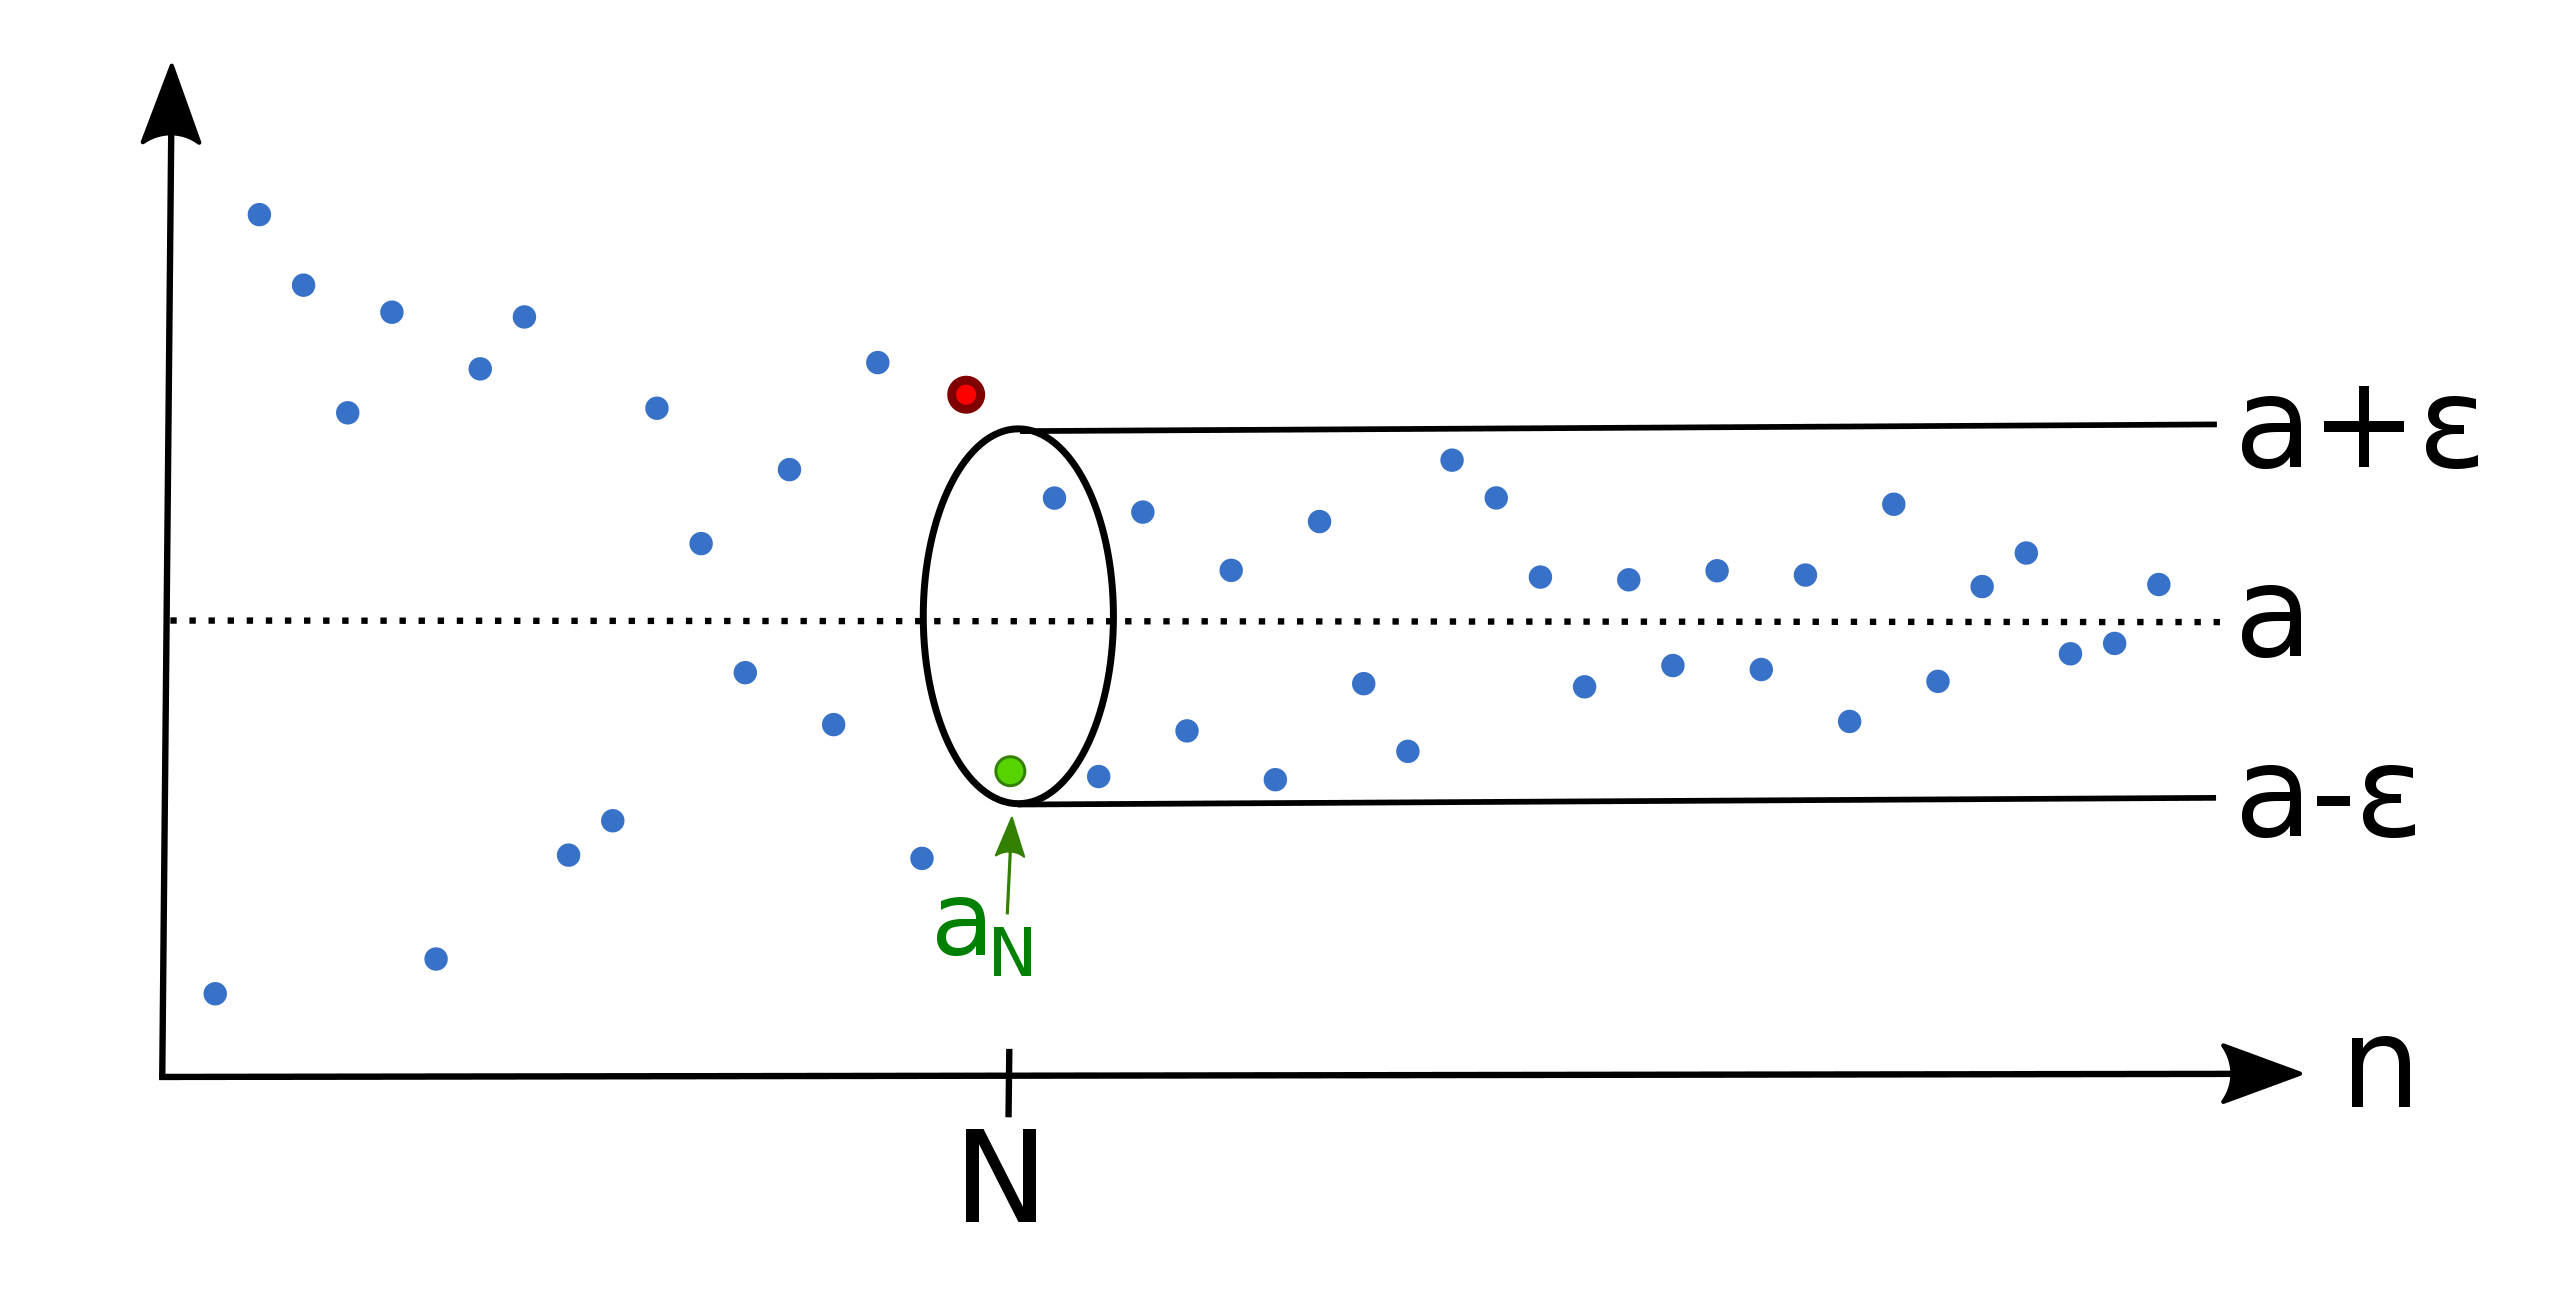
\includegraphics[width=12cm]{conv-seq.png}
			\caption*{All terms after (and including) $a_N$ are contained within the bounds of $a-\varepsilon$ and $a+\varepsilon$.}
		\end{figure}
	\end{fr}
	
	\hfill
	
	\subsubsection*{Drill Exercises}
	
	\paragraph{}
	\inlinebox{green}{\textbf{1}} Determine whether each of the following geometric sequences are converging or diverging.
	
	\begin{multicols}{2}
		\begin{enumerate}[label=\textbf{(\alph*)}]
			\item $\{1, 2, 4, 8, 16,...\}$
			\item $\{400, 200, 100, 50, 25,...\}$
			\item $\{-3^{-1}, 3^{-2}, -3^{-3}, 3^{-4}, -3^{-5}, ...\}$
			\item $\{4, -4, 4, -4, 4,...\}$
			\item $\{-1, -4, -16, -64, -256,...\}$
			\item $\{4, 2, 1, \frac{1}{2}, \frac{1}{4}, ...\}$
		\end{enumerate}
	\end{multicols}
	
	\paragraph{}
	\inlinebox{green}{\textbf{2}} Let $u_n = 2 \cdot 5^n$ and $v_n = \pi^k$ for $n \in \Z^+$. 
	Find the following (write your answers in terms of $\pi$ where appropriate):
	
	\begin{multicols}{2}
		\begin{enumerate}[label=\textbf{(\alph*)}]
			\item $\displaystyle \sum_{k=1}^3 u_k$
			\item $\displaystyle \sum_{k=1}^3 v_k$
			\item $\displaystyle \sum_{k=3}^6 u_k$
			\item $\displaystyle \sum_{k=2}^5 v_k$
			\item $\displaystyle \sum_{k=1}^{4} u_k v_k$
			\item $\displaystyle \sum_{k=1}^{4} \dfrac{u_k}{v_k}$
		\end{enumerate}
	\end{multicols}
	
	\hfill
	
	\subsubsection*{Word Problems}
	
	\paragraph{}
	\inlinebox{green}{\textbf{3}} Let $\{u_n\}$ be a geometric sequence with common ratio $r_u \neq 0$ and
	$\{v_n\}$ be a geometric sequence with common ratio $r_v \neq 0$. Also, let $a \in \R$. Show that:
	
	\begin{enumerate}[label=\textbf{(\alph*)}]
		\item $\{u_n v_n\}$ is a geometric sequence
		\item $\{{u_n}^a\}$ is a geometric sequence
	\end{enumerate}
	
	\paragraph{}
	\inlinebox{green}{\textbf{4}} Let $\{u_n\}$ be a geometric sequence with first term $u_1$ and common ratio $r \neq 0,1$.
	
	Find $u_1$ and $r$, given that:
	
	\begin{enumerate}[label=\textbf{(\alph*)}]
		\item $u_2 = -2u_4$
		\item $u_4 = S_3$
	\end{enumerate}
	
	\paragraph{}
	\inlinebox{yellow}{\textbf{5}} Let $\{u_n\}$ be a geometric sequence with common ratio $r$.\\
	
	Show that $\displaystyle \prod_{k=1}^n u_n = (\sqrt{u_1 u_n})^n$ and explain what conditions for $u_1$ and $r$ must be
	set for this formula to work.\\
	
	\newpage	
	
	\subsection{Infinite geometric series}

	\paragraph{}
	We have looked at convergence of geometric \textit{sequences} and have established that if a common ratio $r$ of a geometric
	sequence is such that $|r| < 1$, then the series converges (otherwise, it diverges). Specifically for a geometric sequence $\{u_n\}$, 
	if $|r| < 1$ then $\displaystyle \lim_{n \to \infty} u_n = 0$. This also implies that the \textbf{series} converges as well, which
	means $\displaystyle \sum_{k=1}^{\infty} u_k$ has a finite value.\\
	
	\begin{pf}
		\begin{theorem*}
			Let $\{u_n\}$ be a geometric sequence with common ratio $r \neq 0$. Then if $|r| < 1$, the \textbf{series} $\{u_n\}$ converges.
		\end{theorem*}
		
		\tcbline
		
		\begin{proof}
			Let $S_n = \displaystyle \sum_{k=1}^n u_k$ and consider the sequence $\{S_n\}$. We want to show that this sequence
			converges.\\
			
			We know that $S_n = \dfrac{u_1 (1 - r^n)}{1 - r}$, so $\displaystyle \sum_{k=1}^\infty u_k = \lim_{n \to \infty} S_n$.\\
			
			$\displaystyle \lim_{n \to \infty} S_n = \lim_{n \to \infty} \dfrac{u_1 (1 - r^n)}{1 - r} = \dfrac{u_1}{1-r} \cdot \lim_{n \to \infty}
			(1-r^n)$\\
			
			Since $|r| < 1$, we have established (in section \textbf{2.2}) that $r^n$ tends to 0 as $n$ approaches infinity. Hence:
			$\displaystyle \lim_{n \to \infty} r^n = 0$, which implies:\\
			
			$\displaystyle \dfrac{u_1}{1-r} \cdot \lim_{n \to \infty} (1-r^n) = \dfrac{u_1}{1-r}$\\
			
			Since this expression is defined (as $r \neq 1$), $S_{\infty}$ exists and thus the series $\{u_n\}$ converges.
		\end{proof}
	\end{pf}
	
	\paragraph{}
	From our convergence proof above, we have found a closed-form expression for $\displaystyle \sum_{k=1}^\infty u_k$:\\
	
	\begin{kp}[Infinite geometric series]
		For a geometric series $\{u_n\}$ with first term $u_1$ and common ratio $r$, if $|r| < 1$ then 
		$$S_{\infty} = \displaystyle \sum_{k=1}^\infty u_k = \dfrac{u_1}{1-r}$$
	\end{kp}
	
	\paragraph{}
	We can consider an example. Let $u_n = \dfrac{3}{2^{n-1}}$. Then $u_1 = 3$ and $r = |r|$\\ $=\dfrac{1}{2} < 1$. Hence,
	$S_{\infty} = \dfrac{3}{1-\frac{1}{2}} = 6$.\\
	
	\stepcounter{excount}
	\begin{ex}
		Let $u_n = \dfrac{5}{(-3)^{n-1}}$ denote the $n$'th term of a geometric sequence. Find $S_\infty$, the sum to infinity of 
		$\{u_n\}$.
		
		\hfill
		\tcbline
		\hfill
		
		$u_1 = 5$ and $r = -\dfrac{1}{3}$. It's clear that $|r| = \dfrac{1}{3} < 1$. Hence:\\
		
		$S_\infty = \dfrac{5}{1+\frac{1}{3}} = \dfrac{15}{4}$
	\end{ex}
	
	\paragraph{}
	For situations where $|r| \geq 1$, the sum to infinity formula may still give you an answer. Be aware though that this will be false.
	For example, consider $u_n = 2^n$. This obviously diverges to infinity as $n$ approaches infinity. However, $S_\infty = 
	\dfrac{2}{1-2} = -2$, which is absurd! In an exam, be sure to check and state that $|r| < 1$ before finding a sum to infinity (if not 
	already stated in the question). This ensures you have justification for finding a sum to infinity.\\
	
	\begin{fr}[Ces\`{a}ro sums]
		A \textit{Ces\`{a}ro sum} is the limit as $n$ approaches infinity of the mean of the first $n$ \textit{partial sums} of a sequence 
		(if it exists). A partial sum is simply $S_n = \displaystyle \sum_{k=1}^n u_k$ for a sequence $\{u_n\}$. Ces\`{a}ro sums were
		named after the Italian mathematician \textit{Ernesto Ces\`{a}ro}.\\
		
		Consider the sequence $\{1, -1, 1, -1, 1, -1, ...\}$, with $n$'th term $u_n = (-1)^{n-1}$. You can probably deduce (easily) that
		this sequence diverges and hence the series also diverges. However, a Ces\`{a}ro sum $C_s$ exists:
		
		$$S_n = \displaystyle \sum_{k=1}^n u_k = \begin{cases} 1, & n \text{ is odd} \\ 0, & n \text{ is even} \end{cases}$$
		
		$$C_n = \dfrac{1}{n} \sum_{k=1}^n S_k$$
		
		$$\{C_n\} = \left\lbrace 1, \frac{1}{2}, \frac{2}{3}, \frac{1}{2}, \frac{3}{5}, \frac{1}{2}, \frac{4}{7}, ... \right\rbrace$$
		
		$$C_n = \begin{cases} \frac{n+1}{2n}, & n \text{ is odd} \\ \frac{1}{2}, & n \text{ is even} \end{cases}$$
		
		$$\lim_{n \to \infty} \frac{n+1}{2n} = \dfrac{1}{2}$$
		
		Hence, $\displaystyle C_s = \lim_{n \to \infty} C_n = \dfrac{1}{2}$, which is the middle value between $0$ and $1$.\\
		
		Note that this does \textbf{not} imply that the series $\{1, -1, 1, -1, ...\}$ converges! Only that it is \textit{Ces\`{a}ro summable}.\\
		
		There are also sequences which aren't Ces\`{a}ro summable (i.e. a Ces\`{a}ro sum doesn't exist). An example of a sequence with
		this property is $\{1, 2, 4, 8, 16, ...\}$. Is there some criteria for which a sequence is or isn't Ces\`{a}ro summable? It's worth 
		exploring.
	\end{fr}
	
	\subsubsection*{Drill Exercises}
	
	\paragraph{}
	\inlinebox{green}{\textbf{1}} Find the sums to infinity of the following geometric sequences, expressing your answers in exact
	form:
	
	\begin{multicols}{2}
		\begin{enumerate}[label=\textbf{(\alph*)}]
			\item $\{400, 200, 100, 50, 25,...\}$
			\item $\{-3^{-1}, 3^{-2}, -3^{-3}, 3^{-4}, -3^{-5}, ...\}$
			\item $\{4, -2, 1, -\frac{1}{2}, \frac{1}{4},...\}$
			\item $\{\pi, \sqrt{\pi}, 1, \frac{1}{\sqrt{\pi}}, \frac{1}{\pi}, ...\}$
			\item $\{9, 3, 1, \frac{1}{3}, \frac{1}{9},...\}$
			\item $\{40, 20, 10, 1, \frac{1}{10},...\}$
		\end{enumerate}
	\end{multicols}
	
	\subsubsection*{Word Problems}	
	
	\paragraph{}
	\inlinebox{green}{\textbf{3}} Komi drops a rubber ball on the ground from a height of 1.5 m. Each time it bounces back up, it reaches
	$80\%$ of the height reached on the last bounce. Calculate the total distance the ball travels.
	
	\paragraph{}
	\inlinebox{yellow}{\textbf{4}} Using the property of geometric series convergence, show that any number $x$ (where $0 < x < 1$) 
	with a recurring group of decimal digits (i.e. $x = 0.\overline{d_1 d_2 d_3 ... d_n}$) is rational.
	
	\paragraph{}
	\inlinebox{yellow}{\textbf{5}} Use \textbf{question 4} to convert the following decimal numbers to fractional form:
	
	\begin{multicols}{2}
		\begin{enumerate}[label=\textbf{(\alph*)}]
			\item $0.33333333...$
			\item $0.6969696969696969...$
			\item $1.307692307692307692...$
			\item $0.86538461538461538461...$
		\end{enumerate}
	\end{multicols}

	\newpage	
	
	\subsection{Applications: simple and compound interest}
	
	\paragraph{}
	Arithmetic and geometric sequences have applications in the real world. An example is calculating \textit{interest}. This section will
	introduce the concept of interest and how to make such calculations.
	
	\paragraph{}
	If someone wants to take a loan from a bank in order to do something like buy a house, they may do so. However, they must
	pay the bank back at some point in time and usually must pay back \textbf{more} than they loaned. Interest is the charge for
	loaned money; the additional amount you must pay back on top of what you have loaned.
	
	\paragraph{}
	Another situation where interest may apply is when someone makes an investment. They invest a certain amount of money and in 
	time, the money they put in grows. After a certain amount of time, they may withdraw what they have invested and make a profit.
	
	\paragraph{}
	The amount charged on a loan or investment depends on the \textit{interest rate}. This describes the percentage of the initial
	loan or investment (such as $5\%$) which must be paid in specific time intervals (such as yearly or monthly). Note that it may help
	to express the rate as a decimal value rather than a percentage to make calculations easier (e.g. $5\% = 0.05$).
	
	\paragraph{}
	The initial value loaned or invested is called the \textit{principal amount}.
	
	\paragraph{}
	There are two types of interest calculations covered in the course. These types are explained below:\\
	
	\begin{kp}[Simple interest]
		Suppose a principal amount of $\$P$ is loaned/invested at a rate of $r$ (so $100r\%$) for $t$ periods (e.g. $t$ months or 
		$t$ years). Then the \textit{simple interest} $I$ is calculated by:
		
		$$I = Prt$$
		
		and the total amount owed/obtained $A$ is calculated by:
		
		$$A = P + I = P + Prt = P(1+rt)$$
		
		The simple interest is calculated as a fraction $r$ of the principal amount $\$P$ and is constant ($\$Pr$). Multiplying
		this constant by a period $t$ yields the total simple interest after that period of time.
	\end{kp}
	
	\paragraph{}
	Simple interest is usually used for short-term loans. Observe that if $u_t = P(1+r(t-1))$, then $\{u_t\}$ is an arithmetic sequence 
	with first term $P$ and common difference $Pr$.\\
	
	\begin{kp}[Compound interest]
		Suppose a principal amount of $\$P$ is loaned/invested at a rate of $r$ for a period of $t$. Then the \textit{compound interest} 
		is calculated as a percentage of the previously-calculated balance and the total amount owed/obtained $A$ is calculated by:
		
		$$A = P(1+r)^t$$
		
		Additionally, if the interest is compounded $n$ times per period $t$, then $A$ is calculated by:
		
		$$A = P\left(1+\frac{r}{n}\right)^{nt}$$
	\end{kp}	
	
	\paragraph{}
	Compound interest is usually used for long-term loans and grows at a faster rate than simple interest. Observe that if
	$u_t = P\left(1+\frac{r}{n}\right)^{n(t-1)}$, then $\{u_t\}$ is a geometric sequence with first term $P$ and common ratio 
	$\left(1+\frac{r}{n}\right)^n$.
	
	\paragraph{}
	Also, interests can be compounded a fixed number of times during a period. Here are some common frequency terms for a
	period of one year:
	
	\begin{longtable}{|c|c|c|}
		\hline
		\textbf{Term} & \textbf{Meaning} & $\mathbold{n}$\\
		\hhline{|=|=|=|}
		Annually & Once per year & $1$\\
		\hline
		Semi-annually & Twice per year & $2$\\
		\hline
		Quarterly & Four times per year & $4$\\
		\hline
		Monthly & Twelve times per year & $12$\\
		\hline
	\end{longtable}
	
	\stepcounter{excount}
	\begin{ex}
		Simon takes a loan of $\$\num{15000}$ from his bank to buy a car, with a monthly simple interest rate of $5\%$. Calculate 
		how much Simon owes the bank after a year.
		
		\hfill
		\tcbline
		\hfill
		
		Note that the simple interest is calculated monthly for a year. Hence, $t=12$. $r = 0.05$, so using the simple interest formula:\\
		
		$A = P(1+rt) = 15000(1+0.05 \cdot 12) = 24000$\\
		
		Hence, Simon owes the bank $\$\num{24000}$ after a year.
	\end{ex}
	
	\hfill
	
	\stepcounter{excount}
	\begin{ex}
		Chika invests \textyen $\num{11000}$ (Japanese yen) in a bank with an annual compound interest rate of $7\%$, 
		compounded quarterly. Calculate the profit she will make after 10 years. Give your answer correct to the nearest yen.
		
		\hfill
		\tcbline
		\hfill
		
		Total amount after 10 years: \\
		$A = P(1+\frac{r}{n})^{nt} = 11000(1+\frac{0.07}{4})^{4 \cdot 10} = 22017.57$\\
		
		$22017.57 - 11000 = 11017.57$\\

		Hence, the profit Chika makes is \textyen $\num{11018}$ rounded to the nearest yen.
	\end{ex}
	
	\hfill
	
	\begin{fr}[$\mathbold{e}$]
		Consider the compound interest formula:
		$$A = P\left(1+\dfrac{r}{n}\right)^{nt}$$
		
		Suppose $\$1$ is invested into a bank account for a year, compounded $n$ times at a rate of $100\%$:
		$$A = \left(1+\dfrac{1}{n}\right)^n$$
		
		Now try inputting this expression into a calculator for different values of $n \geq 1$:
		
		\begin{longtable}{|c|c|}
			\hline
			$\mathbold{n}$ & $\mathbold{A}$\\
			\hhline{|=|=|}
			$1$ & $2$\\
			\hline
			$2$ & $2.25$\\
			\hline
			$5$ & $2.49$\\
			\hline
			$10$ & $2.59$\\
			\hline
			$20$ & $2.65$\\
			\hline
			$100$ & $2.70$\\
			\hline
			$1000$ & $2.717$\\
			\hline
			$10000$ & $2.718$\\
			\hline
		\end{longtable}
		
		As $n$ is increased, $A$ is indeed getting closer to the constant $\e$. This is actually a \textbf{definition} of $\e$. More
		formally:
		
		$$\e = \lim_{n \to \infty} \left(1+\dfrac{1}{n}\right)^n$$
		
		We shall see other definitions of $\e$ later in the course.		
	\end{fr}
	
	\subsubsection*{Word Problems}
	
	\paragraph{}
	\inlinebox{green}{\textbf{1}} Walker wants to invest $\$6000$ in a bank which provides an annual compound interest rate of
	$r\%$, compounded \textbf{monthly}. Given that Walker's investment doubles in value after 5 years, find the value of $r$
	correct to 3 s.f.
	
	\paragraph{}
	\inlinebox{yellow}{\textbf{2}} Kashif takes a loan of $\$\num{14000}$ from his bank which has an annual compound interest rate of
	$4\%$, compounded at the end of each year. To help pay off his loan, he puts in $\$D$ at the end of every year into a savings 
	account with an annual compound interest rate of $3\%$, also compounded yearly. He starts doing this the same year he takes the loan.
	
	\begin{enumerate}[label=\textbf{(\alph*)}]
		\item Find an expression for the total amount in Kashif's savings account after $n$ years.
		\item Hence find the value of $D$ for which Kashif can pay off his loan after 10 years.
	\end{enumerate}
	
	\newpage
	
\section{Polynomials}

	\paragraph{}
	Polynomials are probably the most fundamental expressions in algebra. In fact, the \textit{Fundamental Theorem of Algebra} is 
	a statement about polynomials. A general polynomial has \textit{variables} and \textit{coefficients}. Some examples are:
	
	\begin{itemize}
		\item $x^3 + 3x^2 - 6x + 4$
		\item $x^2 + 2xy + y^2$
		\item $1$
	\end{itemize}
	
	\paragraph{}
	To remove ambiguity, it helps to identify the variables and coefficients (especially if a polynomial has multiple variables). This
	course will only study polynomials of one variable (usually $x$). These will have the form:
	
	$$a_n x^n + a_{n-1} x^{n-1} + ... + a_1 x + a_0$$

	Where $x \in \R$ is the variable and $\{a_0, a_1, ..., a_n\} \subseteq \R$ are the coefficients (constants in $\R$).
	Of course, we can use another set instead of $\R$ such as $\Z$, $\Q$ or $\C$.
	
	\paragraph{}
	Some common polynomials you may be familiar with are:
	
	\begin{itemize}
		\item $ax + b$ (line)
		\item $ax^2 + bx + c$ (quadratic)
	\end{itemize}

	\paragraph{}
	By setting a polynomial to a variable $y$ or a function $f(x)$, we can plot polynomials on a graph and analyze their behavior. We will 
	have a look at what some of these look like in this chapter.

	\subsection{Lines}
	
	\paragraph{}
	You may (or should) be familiar with what a straight line equation looks like. A line, by definition, is the set of all points $(x,y)$ for which
	$y = mx + c$ (you may be familiar with this form), where $m$ is the \textit{gradient} and $c$ is the $y$-intercept of the line. Of course, 
	$x$ is the variable and $m$ and $c$ are coefficients. This is in fact a type of polynomial, as it has the form described above in the 
	introduction. Here are some examples of straight line equations plotted on a graph:
	
	\begin{figure}[H]
	\centering
	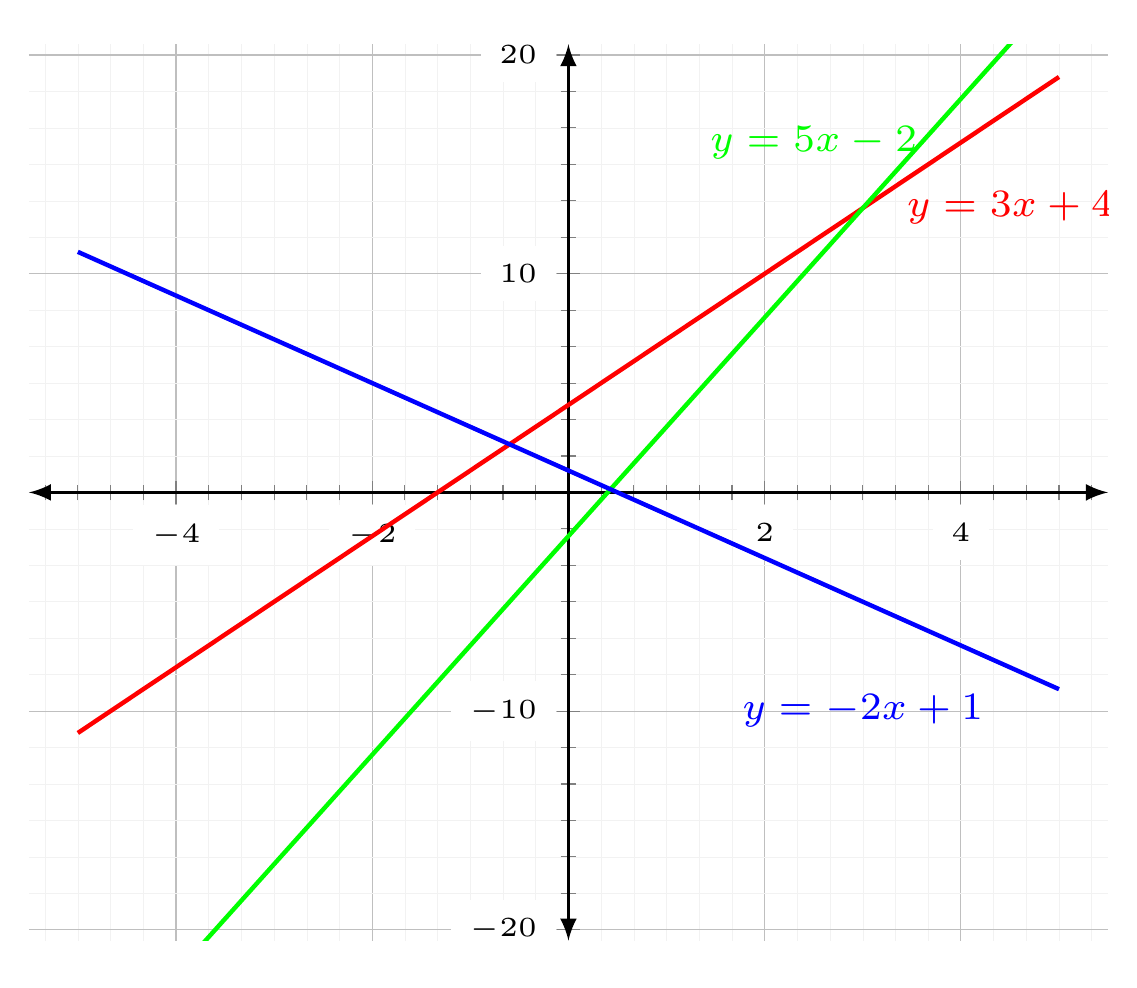
\begin{tikzpicture}[scale=2]
		\begin{axis}[xmin=-5,xmax=5,
							 ymin=-20,ymax=20,
   							 grid=both,
    						 grid style={line width=.1pt, draw=gray!10},
    						 major grid style={line width=.2pt,draw=gray!50},
    						 axis lines=middle,
    						 minor tick num=5,
     						 enlargelimits={abs=0.5},
   							 axis line style={latex-latex},
   							 ticklabel style={font=\tiny,fill=white},
   							 xlabel style={at={(ticklabel* cs:1)},anchor=north west},
   							 ylabel style={at={(ticklabel* cs:1)},anchor=south west}]
		\addplot[mark=none, red, thick, samples=50, domain=-5:5]{3*x+4} node at (axis cs:4.5,13) {\scriptsize $y = 3x+4$};
		\addplot[mark=none, green, thick, samples=50, domain=-5:5]{5*x - 2} node at (axis cs:2.5,16) {\scriptsize $y = 5x - 2$};
		\addplot[mark=none, blue, thick, samples=50, domain=-5:5]{-2*x + 1} node at (axis cs:3,-10) {\scriptsize $y = -2x + 1$};
		\end{axis}
	\end{tikzpicture}
	\end{figure}
	
	\paragraph{}
	You may ask yourself ``where do these coefficients come from and how do they form a straight line?'' Firstly, it may be obvious
	that $c$ is the $y$-intercept because if you set $x=0$, you get $y=c$, which is the point $(0,c)$. Thus, it is the point of the line
	which lies on the $y$-axis. Similarly if you set $y=0$, you get $mx+c = 0$ which implies $x = -\dfrac{c}{m}$ (assuming $m \neq 0$).
	This point $(-\frac{c}{m},0)$ is the point of the line which lies of the $x$-axis.
	
	\paragraph{}
	As for why $m$ is the gradient, we must recall what is meant by a gradient. You may know it as the ``rise over run'' of a line.
	In other words, if you take two \textbf{distinct} points $(x_1, y_1)$ and $(x_2, y_2)$ on a line, the gradient is 
	$m = \dfrac{y_2 - y_1}{x_2 - x_1}$. This describes how much $y$ changes when $x$ changes by 1 unit. In fact, take the point
	$(0, c)$ and the arbitrary point $(x,y)$ (for $x \neq 0$) and observe that:
	
	$$m = \dfrac{y-c}{x-0} = \dfrac{y-c}{x} \implies mx = y - c \implies y = mx + c$$
	
	\paragraph{}
	Indeed, we get the straight line equation. A few other forms of the equation are:
	
	\begin{itemize}
		\item $ax + by + d = 0$ where $a,b,d \in \R$ are constants
		\item $y - y_1 = m(x - x_1)$ where $m$ is the gradient and $(x_1, y_1)$ is a point on the line
	\end{itemize}	 
	
	\paragraph{}
	The derivations of these forms are left as an exercise if you are interested; they are not at all hard to find.\\
	
	\stepcounter{excount}
	\begin{ex}
		Let $m = 3$ be a gradient of a line with a point $(\frac{1}{3},\frac{4}{3})$. Write down the equation of the line in the form 
		$ax + by + d = 0$ where $a,b,d \in \Z$ are constants to be found.
		
		\hfill
		\tcbline
		\hfill
		
		From the form $y - y_1 = m(x-x_1)$, we have that $y - \frac{4}{3} = 3(x - \frac{1}{3})$, so $y = 3x + \frac{1}{3}$.\\
		
		Multiplying both sides by 3, we get $3y = 3x + 1$.\\ 
		
		Thus $3x - 3y + 1 = 0$ or $-3x + 3y - 1 = 0$ (both equations are equivalent).
	\end{ex}
	
	\paragraph{}
	We can also find the point for which two lines $L_1$ and $L_2$ might \textit{intersect}. The procedure is to take two equations:
	$L_1: y = m_1 x + c_1$ and $L_2: y = m_2 x + c_2$ and simply equate the right-hand sides like so: $m_1 x + c_1 = m_2 x + c_2$.
	This means we have equated the $y$ values and must find an $x$ value which satisfies the equation. Then we use our found $x$
	value and plug it back into either of $L_1$ or $L_2$ to find the corresponding $y$ value. To illustrate this, consider the example:\\
	
	\stepcounter{excount}
	\begin{ex}
		Find the point of intersection, $P$, of the two lines $L_1$ and $L_2$ defined by:\\
		$L_1: y = 3x + 5$\\
		$L_2: y = x - 5$\\
		
		\tcbline
		\hfill
		
		Equate the two right-hand sides: $3x + 5 = x - 5$\\
		Then solve for $x$: $2x = -10 \implies x = -5$\\
		Finally, plug this value of $x$ back into $L_1$: $y = 3 \cdot (-5) + 5 = -10$ \\
		
		Hence, the point of intersection is $P(-5, -10)$
	\end{ex}

	\paragraph{}
	You may have noticed (or not) that if two equations had the same gradient, problems may arise when trying to find points
	of intersection. Suppose we have $y = mx + c_1$ and $y = mx + c_2$, both of which have the same gradient $m$. Then equating
	these would yield: $mx + c_1 = mx + c_2 \implies c_1 = c_2$, which wouldn't be a problem as long as $c_1 = c_2$, but clearly
	that's not always the case. If $y = 3x + 4$ and $y = 3x - 5$ and we equate them: $3x + 4 = 3x -5 \implies 4 = -5$, which is a clear
	contradiction. This simply means that the two lines never meet. We denote this as \textit{parallelism} and say that the two lines are
	\textit{parallel} to each other.\\
	
	\begin{kp}[Parallel lines]
		Two lines $L_1: y = m_1 x + c_1$ and $L_2: m_2 x + c_2$ are \textit{parallel} if and only if $m_1 = m_2$ and $c_1 \neq c_2$.
	\end{kp}
	
	Some parallel lines are graphed below:
	
	\begin{figure}[H]
	\centering
	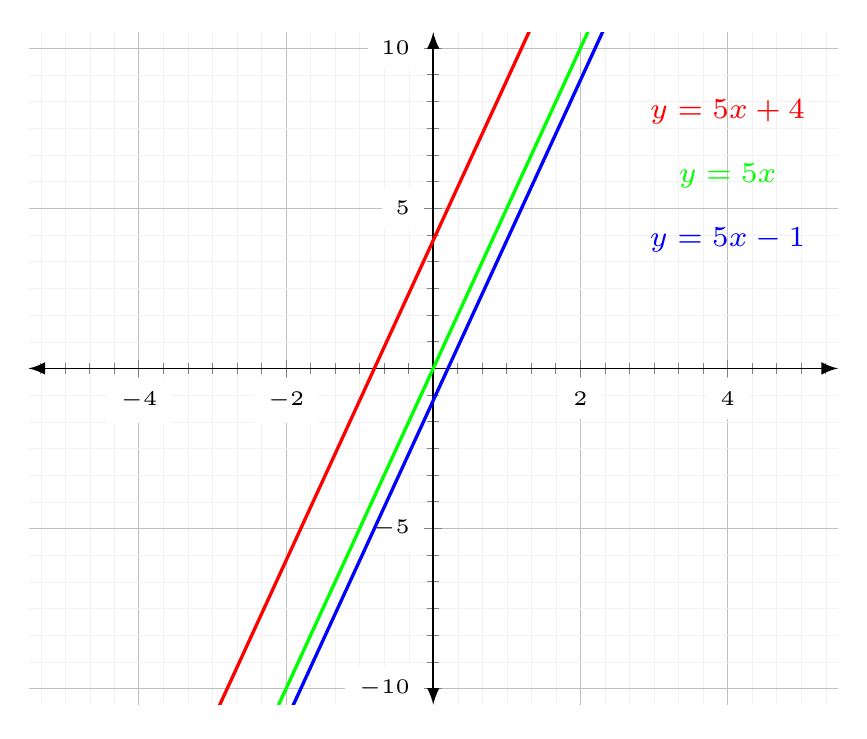
\begin{tikzpicture}[scale=1.5]
		\begin{axis}[xmin=-5,xmax=5,
							 ymin=-10,ymax=10,
   							 grid=both,
    						 grid style={line width=.1pt, draw=gray!10},
    						 major grid style={line width=.2pt,draw=gray!50},
    						 axis lines=middle,
    						 minor tick num=5,
     						 enlargelimits={abs=0.5},
   							 axis line style={latex-latex},
   							 ticklabel style={font=\tiny,fill=white},
   							 xlabel style={at={(ticklabel* cs:1)},anchor=north west},
   							 ylabel style={at={(ticklabel* cs:1)},anchor=south west}]
		\addplot[mark=none, red, thick, samples=50, domain=-3:3]{5*x+4} node at (axis cs:4,8) {\scriptsize $y = 5x+4$};
		\addplot[mark=none, green, thick, samples=50, domain=-3:3]{5*x} node at (axis cs:4,6) {\scriptsize $y = 5x$};
		\addplot[mark=none, blue, thick, samples=50, domain=-3:3]{5*x - 1} node at (axis cs:4,4) {\scriptsize $y = 5x - 1$};
		\end{axis}
	\end{tikzpicture}
	\end{figure}
	
	\paragraph{}
	If two lines are such that they meet at a right angle, we say they are \textit{perpendicular}. There is indeed a gradient condition
	for this property to hold:\\
	
	\begin{kp}[Perpendicular lines]
		Two lines $L_1: y = m_1 x + c_1$ and $L_2: m_2 x + c_2$ are \textit{perpendicular} if and only if $m_1 m_2 = -1$.
	\end{kp}
	
	Two perpendicular lines are graphed below:
	
	\begin{figure}[H]
	\centering
	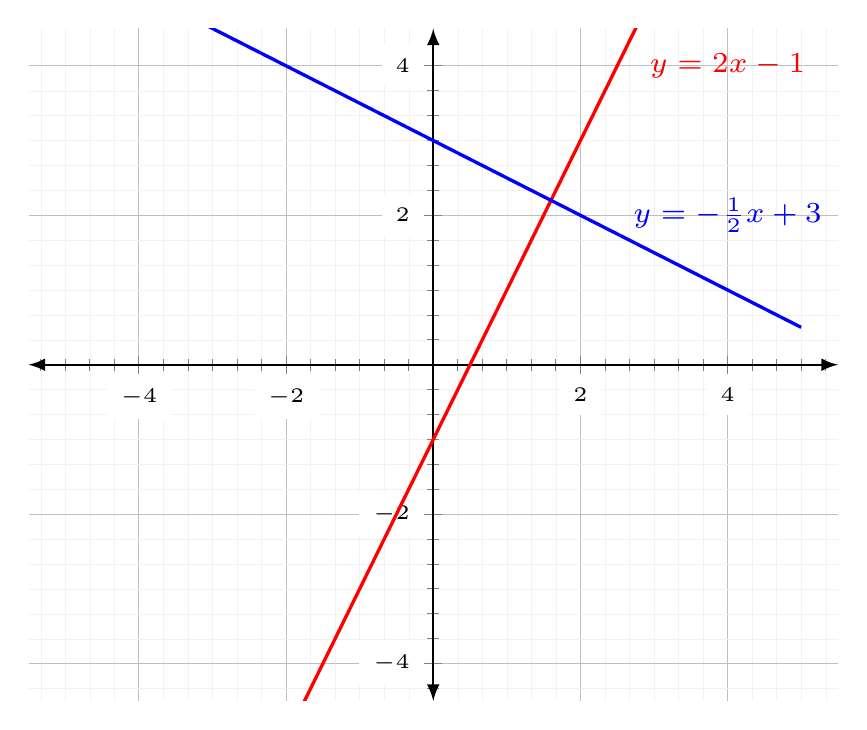
\begin{tikzpicture}[scale=1.5]
		\begin{axis}[xmin=-5,xmax=5,
							 ymin=-4,ymax=4,
   							 grid=both,
    						 grid style={line width=.1pt, draw=gray!10},
    						 major grid style={line width=.2pt,draw=gray!50},
    						 axis lines=middle,
    						 minor tick num=5,
     						 enlargelimits={abs=0.5},
   							 axis line style={latex-latex},
   							 ticklabel style={font=\tiny,fill=white},
   							 xlabel style={at={(ticklabel* cs:1)},anchor=north west},
   							 ylabel style={at={(ticklabel* cs:1)},anchor=south west}]
		\addplot[mark=none, red, thick, samples=50, domain=-5:5]{2*x-1} node at (axis cs:4,4) {\scriptsize $y = 2x-1$};
		\addplot[mark=none, blue, thick, samples=50, domain=-5:5]{-0.5*x +3} node at (axis cs:4,2) {\scriptsize $y = -\frac{1}{2}x + 3$};
		\end{axis}
	\end{tikzpicture}
	\end{figure}
	
	\paragraph{}
	The proof of the perpendicular line fact is given below (you will \textbf{not} need to know it for the exam):\\
	
	\begin{pf}
		\begin{theorem*}
			For two lines $L_1: y = m_1 x + c_1$ and $L_2: y = m_2 x  + c_2$ ($m_1, m_2 \neq 0$), \\ $L_1$ and $L_2$ are perpendicular 
			if and only if $m_1 m_2 = -1$
		\end{theorem*}
		
		\tcbline
		
		\begin{proof} \textit{Note: $\iff$ means `if and only if'}\\
			Suppose $L_1$ and $L_2$ meet at a right angle:\\
			
		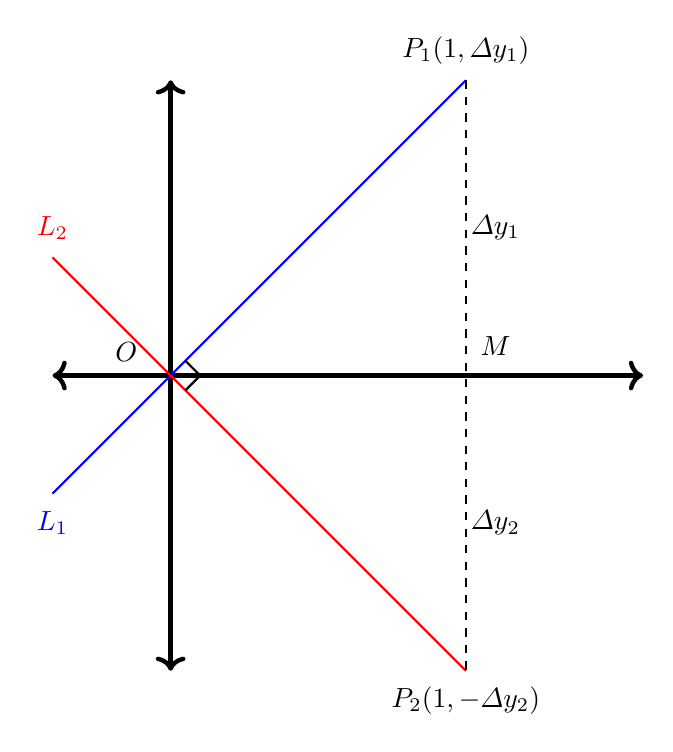
\begin{tikzpicture}[scale=0.75]
			\draw[ultra thick,->] (0,0) -- (8,0);
			\draw[ultra thick,->] (0,0) -- (-2,0);
			\draw[ultra thick,->] (0,0) -- (0,5);
			\draw[ultra thick,->] (0,0) -- (0,-5);
			\draw[color=blue, thick] (-2,-2) -- (5,5) node at (-2,-2.5) {$L_1$};
			\draw[color=red, thick] (-2,2) -- (5,-5) node at (-2,2.5) {$L_2$};
			\draw[dashed, thick] (5,5) -- (5,-5);
			\draw[thick] (0.25, 0.25) -- (0.5, 0) -- (0.25, -0.25);
			\node at (5, 5.5) {$P_1(1,\Delta y_1)$};
			\node at (5, -5.5) {$P_2(1,-\Delta y_2)$};
			\node at (5.5,2.5) {$\Delta y_1$};
			\node at (5.5,-2.5) {$\Delta y_2$};
			\node at (-0.75, 0.4) {$O$};
			\node at (5.5, 0.5) {$M$};
		\end{tikzpicture}
			
		Where $m_1 = \Delta y_1$ and $m_2 = -\Delta y_2$.\\
		
		By Pythagoras' theorem, $OP_1 = \sqrt{{\Delta y_1}^2 + 1}$ and $OP_2 = \sqrt{{\Delta y_2}^2 + 1}$.\\
		
		Also, ${(OP_1)}^2 + {(OP_2)}^2 = (\Delta y_1 + \Delta y_2)^2$\\
		
		$\iff {(\Delta y_1)}^2 + 1 + {(\Delta y_2)}^2 + 1 = {(\Delta y_1)}^2 + {(\Delta y_2)}^2 + 2{(\Delta y_1)}{(\Delta y_2)}$\\
		
		$\iff 2{(\Delta y_1)}{(\Delta y_2)} = 2$\\
		
		$\iff m_1 (-m_2) = 1$\\
		
		$\iff m_1 m_2 = -1$ as required.\\
		
		The converse clearly holds due to equality of the statements, so the theorem must be true.
		\end{proof}
	\end{pf}
	
	\hfill	
	
	\stepcounter{excount}
	\begin{ex}
		Let $L_1: y = kx + 4$ and $L_2: y = 2x + 3$. Find the value of $k$ for which:
		
		\begin{enumerate}[label=\textbf{(\alph*)}]
			\item $L_1$ and $L_2$ are parallel
			\item $L_1$ and $L_2$ are perpendicular
		\end{enumerate}
		
		\tcbline
		\hfill
		
		\begin{enumerate}[label=\textbf{(\alph*)}]
			\item We have that $4 \neq 3$, so we need $k = 2$ for the lines to be parallel.
			\item We must have that $2k = -1 \implies k = -\dfrac{1}{2}$ for the lines to be perpendicular.
		\end{enumerate}
	\end{ex}	
	
	\newpage
	
	\begin{fr}[Equivalence relations]
		There is some debate on whether on not we need the condition that $c_1 \neq c_2$. That is, whether a line is \textbf{parallel to itself}.
		Euclid (the 300 BC Greek mathematician and founder of geometry) has defined parallelism such that a line can't be parallel to itself. 
		However, others have allowed lines to be parallel to themselves so that parallelism could be an \textit{equivalence relation}. \\
		
		What we mean by a relation is an operator which describes how two (or more) objects are related. For example, equality $(=)$ is a 
		relation between two values $x$ and $y$ (if $x=y$, we say $x$ is related to $y$ by equality). Other relations include $>$ and 
		$\equiv$.\\
		
		A relation $R$ is an \textit{equivalence relation} if $R$ is \textit{reflexive} ($xRx$), \textit{symmetric} ($xRy \implies yRx$) and 
		\textit{transitive} ($xRy \text{ and } yRz \implies xRz$) for all values $x,y,z$ in a specified set. It is obvious that $=$ is an equivalence 
		relation, but not $>$ (since it isn't reflexive or symmetric).\\
		
		As for parallelism, denote the relation to be $\Vert$ (i.e. $L_1 \; \Vert \; L_2$ means the lines $L_1$ and $L_2$ are parallel) and
		suppose we say that for $L_1: y = m_1 x + c_1$ and $L_2: y = m_2 x + c_2$, $L_1 \; \Vert \; L_2$ if and only if $m_1 = m_2$. 
		Let $L_3 = m_3 x + c_3$. Then we have:\\
		
		\textbf{Reflexivity:} $L_1 \; \Vert \; L_1 \implies m_1 = m_1$, which is clearly true.\\
		
		\textbf{Symmetry:} $L_1 \; \Vert \; L_2 \implies m_1 = m_2 \implies m_2 = m_1 \implies L_2 \; \Vert \; L_1$.\\
		
		\textbf{Transitivity:} $L_1 \; \Vert \; L_2 \implies m_1 = m_2$ and $L_2 \; \Vert \; L_3 \implies m_2 = m_3 \implies
		m_1 = m_2 = m_3 \implies m_1 = m_3 \implies L_1 \; \Vert \; L_3$\\
		
		By that definition of parallelism, it is indeed an equivalence relation. However, you can see that the reflexive property doesn't
		hold when we introduce the condition that $c_1 \neq c_2$.
	\end{fr}
	
	\subsubsection*{Drill Exercises}
	
	\paragraph{}
	\inlinebox{green}{\textbf{1}} Convert the following line equations to the form $ax + by + d = 0$ where $a,b,d \in \Z$.
	
	\begin{multicols}{2}
		\begin{enumerate}[label=\textbf{(\alph*)}]
			\item $y = 3x + 4$
			\item $y = \dfrac{5}{4}x - 1$
			\item $y = \dfrac{3}{8}x - \dfrac{2}{3}$
			\item $y - 3 = 4(x-1)$
			\item $y + 3 = 2(x+5)$
			\item $\sqrt{2}y +\dfrac{\sqrt{2}}{2} x = \dfrac{1}{\sqrt{2}}$
		\end{enumerate}
	\end{multicols}
	
	\subsubsection*{Word Problems}	
	
	\paragraph{}
	\inlinebox{green}{\textbf{3}} While the proof of perpendicularity shown above is correct, it assumes that the gradients of the
	lines are non-zero. If \textbf{one} of the lines has a gradient of zero (i.e. $L_1: y = c_1$), explain what equation the other line $L_2$ 
	must have for $L_1$ and $L_2$ to be perpendicular.
	
	\paragraph{}
	\inlinebox{yellow}{\textbf{2}} Given any arbitrary point $(x_1, y_1)$ and a gradient $m \neq 0$, explain how a straight line
	equation of the form $y = mx + c$ can be found and prove that this line is unique (that is, no other line of the same gradient can
	pass through that point).
	
	\hfill

	\subsection{Quadratics}
	
	\paragraph{}
	A quadratic is a polynomial of the form $ax^2 + bx + c = 0$ where $a \neq 0$. If $a=0$, clearly we would have a straight line.
	Some quadratics are plotted below:\\
	
	\begin{figure}[H]
	\centering
	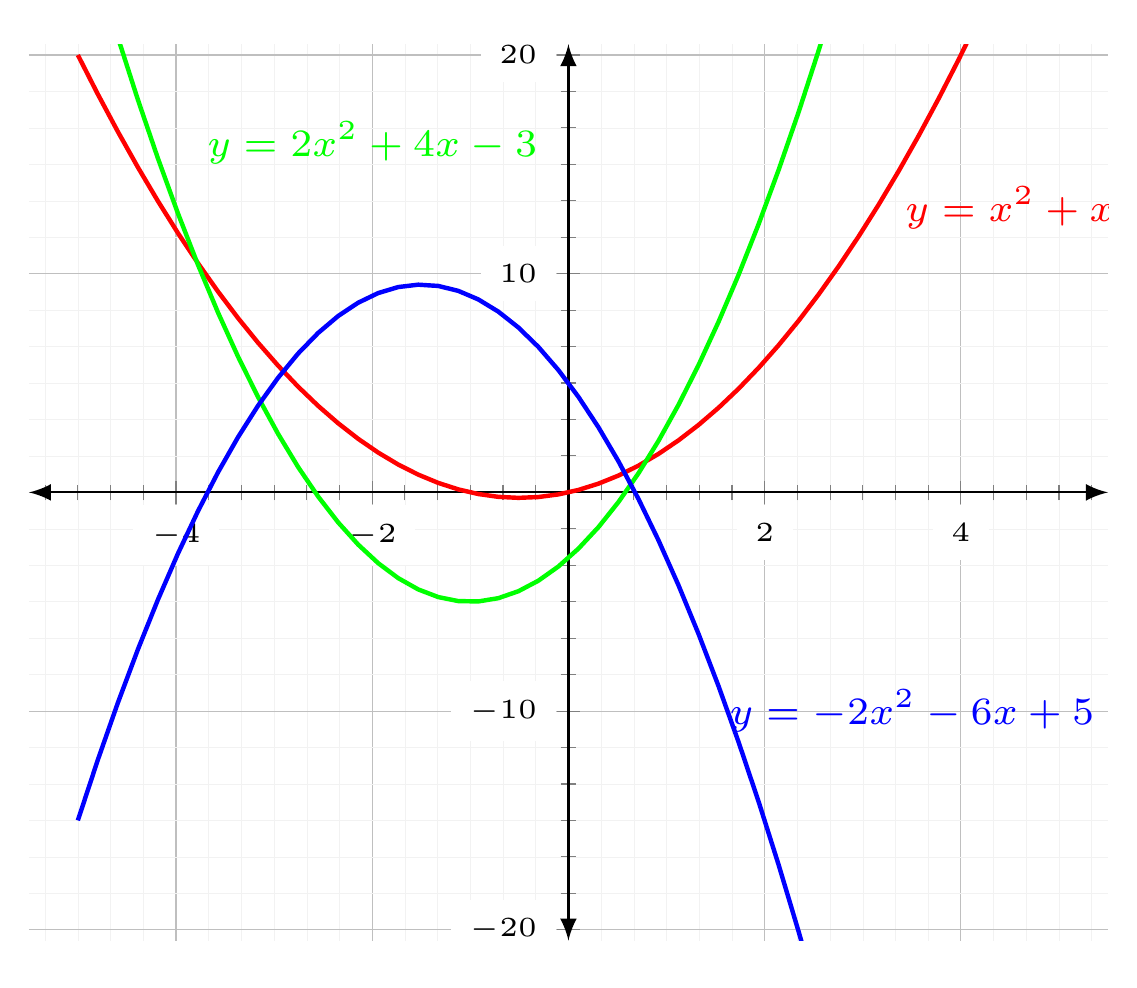
\begin{tikzpicture}[scale=2]
		\begin{axis}[xmin=-5,xmax=5,
							 ymin=-20,ymax=20,
   							 grid=both,
    						 grid style={line width=.1pt, draw=gray!10},
    						 major grid style={line width=.2pt,draw=gray!50},
    						 axis lines=middle,
    						 minor tick num=5,
     						 enlargelimits={abs=0.5},
   							 axis line style={latex-latex},
   							 ticklabel style={font=\tiny,fill=white},
   							 xlabel style={at={(ticklabel* cs:1)},anchor=north west},
   							 ylabel style={at={(ticklabel* cs:1)},anchor=south west}]
		\addplot[mark=none, red, thick, samples=50, domain=-5:5]{x^2+x} node at (axis cs:4.5,13) {\scriptsize $y = x^2 + x$};
		\addplot[mark=none, green, thick, samples=50, domain=-5:5]{2*x^2 + 4*x - 3} node at (axis cs:-2,16) 
		{\scriptsize $y = 2x^2 + 4x - 3$};
		\addplot[mark=none, blue, thick, samples=50, domain=-5:5]{-2*x^2 - 6*x + 5} node at (axis cs:3.5,-10) 
		{\scriptsize $y = -2x^2 - 6x + 5$};
		\end{axis}
	\end{tikzpicture}
	\end{figure}
	
	\paragraph{}
	From an analytic point of view, there is a lot more to quadratics than straight lines. You will notice that quadratics have a variable
	gradient for starters (we will see how we can obtain this using calculus later on). Another is that quadratics in $\R$ will not span
	the whole of $\R$. That is, every quadratic in $\R$ has either a least value or a greatest value (the point with this value is called
	the \textit{vertex}.\\
	
	\begin{kp}[Vertex of a quadratic]
		For a quadratic $ax^2 + bx + c$, the vertex is the point for which the quadratic attains a maximum (when $a < 0$) or minimum
		(when $a > 0$) value. It is also the only point on the quadratic for which the gradient is 0.
	\end{kp}
	
	\paragraph{}
	The vertex for the quadratic equation $y = 2x^2 + 4x + 4$ is shown below:
	
	\begin{figure}[H]
	\centering
	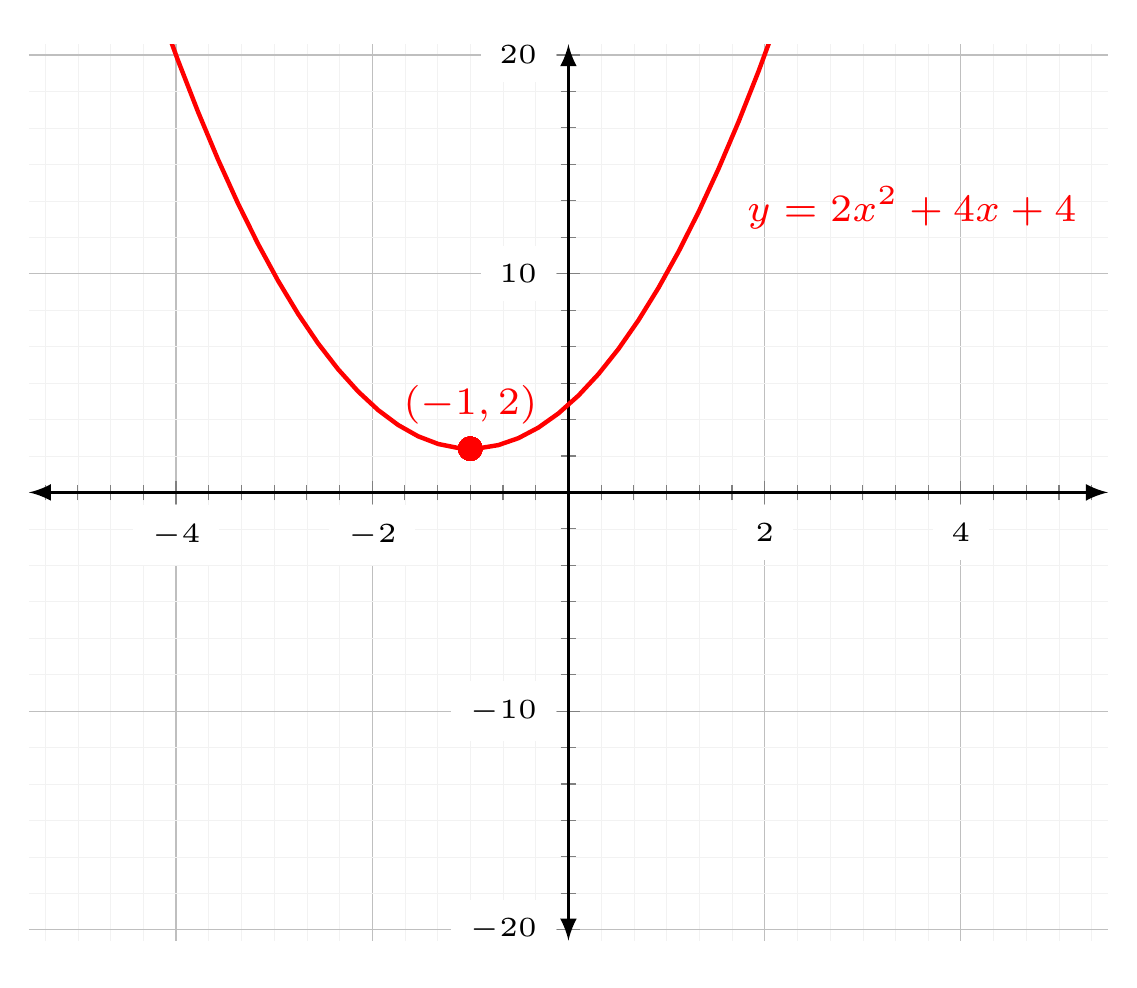
\begin{tikzpicture}[scale=2]
		\begin{axis}[xmin=-5,xmax=5,
							 ymin=-20,ymax=20,
   							 grid=both,
    						 grid style={line width=.1pt, draw=gray!10},
    						 major grid style={line width=.2pt,draw=gray!50},
    						 axis lines=middle,
    						 minor tick num=5,
     						 enlargelimits={abs=0.5},
   							 axis line style={latex-latex},
   							 ticklabel style={font=\tiny,fill=white},
   							 xlabel style={at={(ticklabel* cs:1)},anchor=north west},
   							 ylabel style={at={(ticklabel* cs:1)},anchor=south west}]
		\addplot[mark=none, red, thick, samples=50, domain=-5:5]{2*x^2+4*x+4} node at (axis cs:3.5,13) {\scriptsize $y = 2x^2 + 4x + 4$};
		\addplot[only marks, red] (-1, 2) node at (axis cs: -1, 4) {\scriptsize $(-1, 2)$};
		\end{axis}
	\end{tikzpicture}
	\end{figure}
	
	\paragraph{}
	There is a way to obtain the exact coordinates of a vertex algebraically using a quadratic expression. It involves a process you may be
	familiar with called \textit{completing the square}.\\
	
	\begin{kp}[Completing the square]
		A quadratic of the form $ax^2 + bx + c$ (for $a,b,c \in \R$, $a \neq 0$) can be written in the form $a(x-h)^2 + k$ (for $h,k \in \R$)
		where the vertex has coordinates $(h,k)$. The process is as follows:
		
		\begin{enumerate}
			\item Factor out the coefficient $a$ from the $x^2$ and $x$ terms: $a(x^2 + \frac{b}{a}x) + c$
			\item Notice that $(x+\frac{b}{2a})^2 = x^2 + \frac{b}{a}x + (\frac{b}{2a})^2$
			\item Hence $x^2 + \frac{b}{a}x$ can be written as $(x+\frac{b}{2a})^2 - (\frac{b}{2a})^2$
			\item Hence the quadratic can be written as $a((x+\frac{b}{2a})^2 - (\frac{b}{2a})^2) + c$
			\item Multiply $a$ and simplify (if needed): $a(x+\frac{b}{2a})^2 - \frac{b^2}{4a} + c$
			\item The vertex will have coordinates $(-\frac{b}{2a}, c - \frac{b^2}{4a})$
		\end{enumerate}
	\end{kp}
	
	\paragraph{}
	Notice the $-h$ in the expression and take care when writing down the coordinates of the vertex (for example, a quadratic
	$2(x+3)^2 + 2$ will have its vertex at $(-3, 2)$).\\
	
	\stepcounter{excount}
	\begin{ex}
		Let $y = 3x^2 - 6x + 2$ be a quadratic equation.
		
		\begin{enumerate}[label=\textbf{(\alph*)}]
			\item Convert the quadratic to completed square form.
			\item Hence write down the coordinates of its vertex.
		\end{enumerate}
		
		\hfill
		\tcbline
		\hfill
		
		\begin{enumerate}[label=\textbf{(\alph*)}]
			\item $3x^2 - 6x + 2$\\
			
			$= 3(x^2 - 2x) + 3$\\
			
			$= 3((x-1)^2 - 1) + 3$\\
			
			$= 3(x-1)^2$

			\item The vertex has coordinates: $(1, 0)$ 
		\end{enumerate}
	\end{ex}
	
	\paragraph{}
	We can also \textit{factorize} some quadratics by writing them in the form $a(x-p)(x-q)$ where $a, p, q \in \R (a \neq 0)$.
	Not all quadratics in $\R$ have this property (but they all do in $\C$). Factorizing is a skill which takes some intuition and
	a bit of ``trial and error''. By setting the factorized quadratic to zero, we can easily find values of $x$ for which the quadratic 
	is zero (these will clearly be $x=p$ and $x=q$ and $p$ and $q$ could be the same value as well). We call these the \textit{roots} 
	or the \textit{zeros} of the quadratic. This key point may help:\\
	
	\begin{kp}[Product and sum of quadratic roots]
		For a quadratic $ax^2 + bx + c$ with roots $p$ and $q$:
		
		\begin{itemize}
			\item $pq = \frac{c}{a}$
			\item $p+q = \frac{b}{a}$
		\end{itemize}
		
		Note that these formulas will still hold even when $p=q$, and the roots will be counted twice.
	\end{kp}
	
	\paragraph{}
	This fact is easy to see when multiplying out the quadratic's factorized form and equating the coefficients. Some roots  of a quadratic are
	shown below on a graph:\\
	
	\begin{figure}[H]
	\centering
	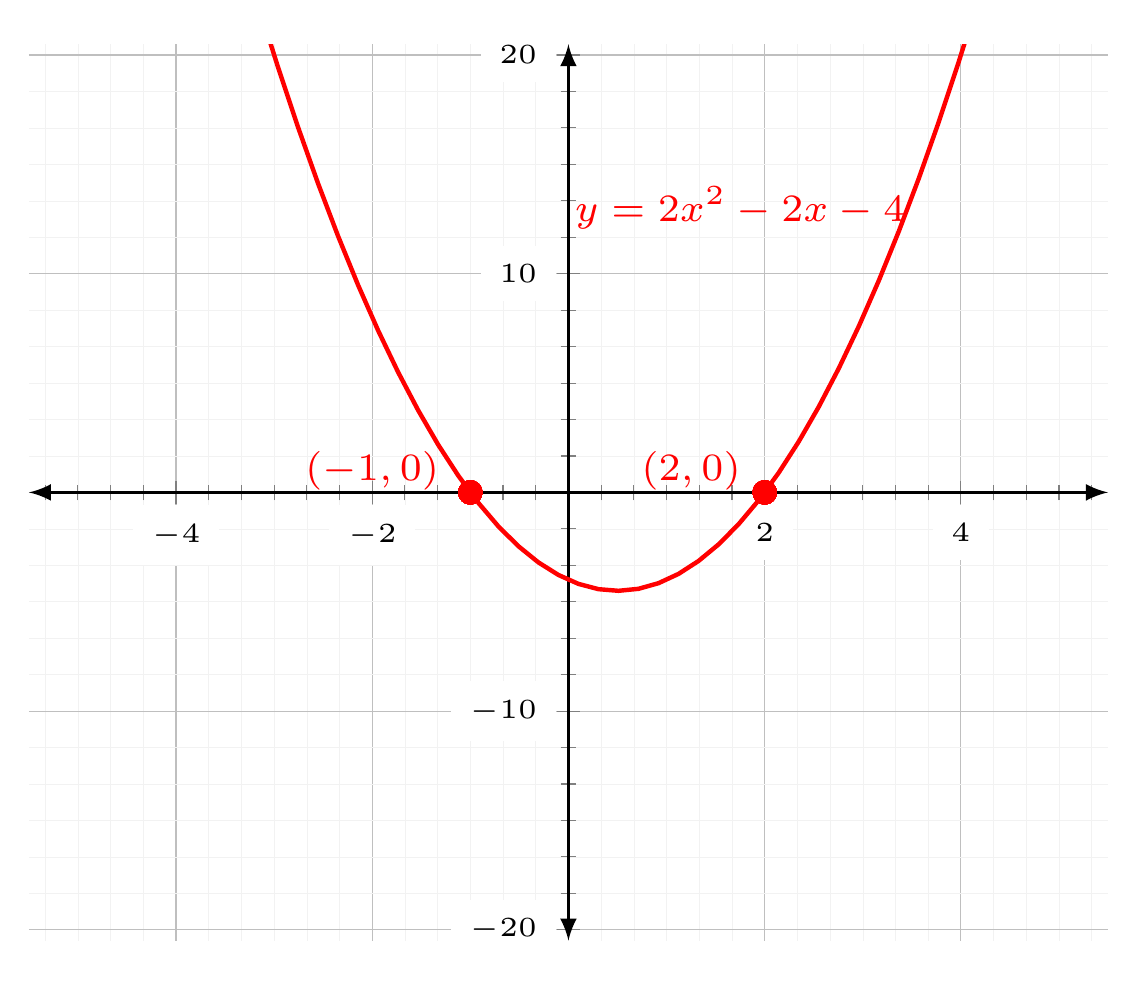
\begin{tikzpicture}[scale=2]
		\begin{axis}[xmin=-5,xmax=5,
							 ymin=-20,ymax=20,
   							 grid=both,
    						 grid style={line width=.1pt, draw=gray!10},
    						 major grid style={line width=.2pt,draw=gray!50},
    						 axis lines=middle,
    						 minor tick num=5,
     						 enlargelimits={abs=0.5},
   							 axis line style={latex-latex},
   							 ticklabel style={font=\tiny,fill=white},
   							 xlabel style={at={(ticklabel* cs:1)},anchor=north west},
   							 ylabel style={at={(ticklabel* cs:1)},anchor=south west}]
		\addplot[mark=none, red, thick, samples=50, domain=-5:5]{2*x^2 - 2*x - 4} node at (axis cs:1.75,13) {\scriptsize $y = 2x^2 - 2x - 4$};
		\addplot[only marks, red] (-1, 0) node at (axis cs: -2, 1) {\scriptsize $(-1, 0)$};
		\addplot[only marks, red] (2, 0) node at (axis cs: 1.25, 1) {\scriptsize $(2, 0)$};
		\end{axis}
	\end{tikzpicture}
	\end{figure}
	
	\stepcounter{excount}
	\begin{ex}
		By factorizing $x^2 + 5x + 6$, find the values of $x$ for which $x^2 + 5x + 6 = 0$.
		
		\hfill
		\tcbline
		\hfill
		
		Let $x^2 + 5x + 6 = a(x-p)(x-q)$. Since $a = 1$, we know that $pq = 6$ and $p+q=3$.
		By intuition, $p = 3$ and $q = 2$. Hence, the roots are $x = 3$ and $x = 2$.
	\end{ex}
	
	\paragraph{}
	If a particular quadratic looks difficult to factorize, you can complete the square to solve for the roots:\\
	
	\stepcounter{excount}
	\begin{ex}
		Find the roots of $x^2 + x - 1$ in exact form.
		
		\hfill
		\tcbline
		\hfill
		
		Complete the square:\\ $x^2 + x - 1$\\ $= (x+\frac{1}{2})^2 - (\frac{1}{2})^2 - 1$\\ $= (x+\frac{1}{2})^2 - \frac{5}{4}$\\
		
		Set the expression to 0 and solve for $x$:\\
		$(x+\frac{1}{2})^2 - \frac{5}{4} = 0$\\
		$(x+\frac{1}{2})^2 = \frac{5}{4}$\\
		$x+\frac{1}{2} = \pm \frac{\sqrt{5}}{2}$ (since squaring a negative number gives a positive number)\\
		$x = \frac{-1 \pm \sqrt{5}}{2}$\\
		
		Hence the roots are $x = \dfrac{\sqrt{5} - 1}{2}$ and $x = -\dfrac{\sqrt{5} + 1}{2}$
	\end{ex}
	
	\paragraph{}
	You may find it helpful to plug the roots you've found back into the original equation. The expression will evaluate to 0 if you've found 
	the correct ones. You can also find a factorized expression for a quadratic using the roots found. For the above example, the quadratic
	$x^2 + x - 1$ can be written as $\left(x-\frac{\sqrt{5} - 1}{2}\right)\left(x+\frac{\sqrt{5} + 1}{2}\right)$.
	
	\paragraph{}
	While completing the square is one way of finding quadratic roots, there is a method to obtain them directly which comes from this 
	process. This is a formula in terms of quadratic coefficients called the \textit{quadratic formula} which you may be familiar with already. 
	Here's the formula and the proof:\\
	
	\begin{pf}
		\begin{theorem*}
			For a quadratic of the form $ax^2 + bx + c$ where $a \neq  0$, the roots are:
			$$\dfrac{-b \pm \sqrt{b^2 - 4ac}}{2a}$$
		\end{theorem*}
		
		\tcbline	
		
		\begin{proof}
			Start with $ax^2 + bx + c$ and complete the square to obtain:\\
			
			$a\left(x+\dfrac{b}{2a}\right)^2 - \dfrac{b^2}{4a} + c$\\
			
			Set this expression to 0 and solve for $x$:\\
			
			$a\left(x+\dfrac{b}{2a}\right)^2 - \dfrac{b^2}{4a} + c = 0$\\
			
			$a\left(x+\dfrac{b}{2a}\right)^2 = \dfrac{b^2}{4a} - c$\\
			
			$a\left(x+\dfrac{b}{2a}\right)^2 = \dfrac{b^2 - 4ac}{4a}$\\
			
			$\left(x+\dfrac{b}{2a}\right)^2 = \dfrac{b^2 - 4ac}{4a^2}$\\
			
			$x+\dfrac{b}{2a} = \pm \dfrac{\sqrt{b^2 - 4ac}}{2a}$\\
			
			$x = \dfrac{-b \pm \sqrt{b^2 - 4ac}}{2a}$
		\end{proof}
	\end{pf}
	
	\paragraph{}
	This equations works for any quadratic in $\R$ or even $\C$ as long as $a \neq 0$.
	
	\paragraph{}
	We can now analyze the quadratic equation; in particular the expression $b^2 - 4ac$. We call this the \textit{discriminant}
	and use the variable $\Delta$ (i.e. $\Delta = b^2 - 4ac$).\\
	
	\begin{kp}[Discriminant of a quadratic]
		For a quadratic $ax^2 + bx + c$, the \textit{discriminant} $\Delta = b^2 - 4ac$ can be used to determine the nature of the quadratic
		roots as follows:
		
		\begin{itemize}
			\item If $\Delta > 0$, there are exactly \textbf{two distinct real roots}.
			\item If $\Delta = 0$, there is exactly \textbf{one real root} (a repeated root).
			\item If $\Delta < 0$, there are \textbf{no real roots}.
		\end{itemize}
	\end{kp}
	
	\paragraph{}
	This is quite clear to see due to the symmetry of the square root in the quadratic equation. Also, the square root of a
	negative number is undefined in $\R$, so $\Delta < 0$ results in no real roots.\\
	
	\stepcounter{excount}
	\begin{ex}
		Consider the quadratic $kx^2 + (k-1)x + (k-1)$. Find the range of values of $k$ for which the quadratic has exactly two 
		distinct real roots.
		
		\hfill
		\tcbline
		\hfill
		
		We can use the discriminant condition that $\Delta > 0$:\\ 
		$\Delta = (k-1)^2 - 4(k)(k-1)$\\
		$= (k-1)(k-1-4k)$\\
		$= (1-k)(3k+1)$\\
		
		Then: $(1-k)(3k+1) > 0$, so either:
		\begin{enumerate}
			\item $1-k > 0$ and $3k+1 > 0$
			\item $1-k < 0$ and $3k+1 < 0$
		\end{enumerate}
		\hfill
		
		For the first case, $k < 1$ and $k > -\frac{1}{3}$\\
		
		For the second case, $k > 1$ and $k < -\frac{1}{3}$, which is not possible\\
		
		Hence, the range of values of $k$ for which the quadratic has exactly two roots is $-\frac{1}{3} < k < 1$
	\end{ex}
	
	\paragraph{}
	Speaking of symmetry, the vertex's $x$-value gives the equation of the \textit{axis of symmetry} of a quadratic. This denotes
	the line of symmetry for a quadratic graph.\\
	
	\begin{kp}[Axis of symmetry]
		For a quadratic $ax^2 + bx + c$, the \textit{axis of symmetry} is the line $x = -\dfrac{b}{2a}$
	\end{kp}	
	
	\stepcounter{excount}
	\begin{ex}
		Consider the quadratic $3x^2 - 12x + 13$.
		
		\begin{enumerate}[label=\textbf{(\alph*)}]
			\item Express the quadratic in completed square form
			\item Hence write down the equation of the quadratic's axis of symmetry
			\item Hence sketch the graph of $y = 3x^2 - 12x + 13$ and draw the axis of symmetry.
		\end{enumerate}
		
		\hfill
		\tcbline
		\hfill
		
		\begin{enumerate}[label=\textbf{(\alph*)}]
			\item $3x^2 - 12x + 13$\\
			$= 3(x^2 - 4x) + 13$\\
			$= 3((x-2)^2 - 4) + 13$\\
			$= 3(x-2)^2 + 1$
			
			\item The equation of the axis of symmetry is $x = 2$
			
			\item The graph is shown below:
			
			\begin{figure}[H]
			\centering
			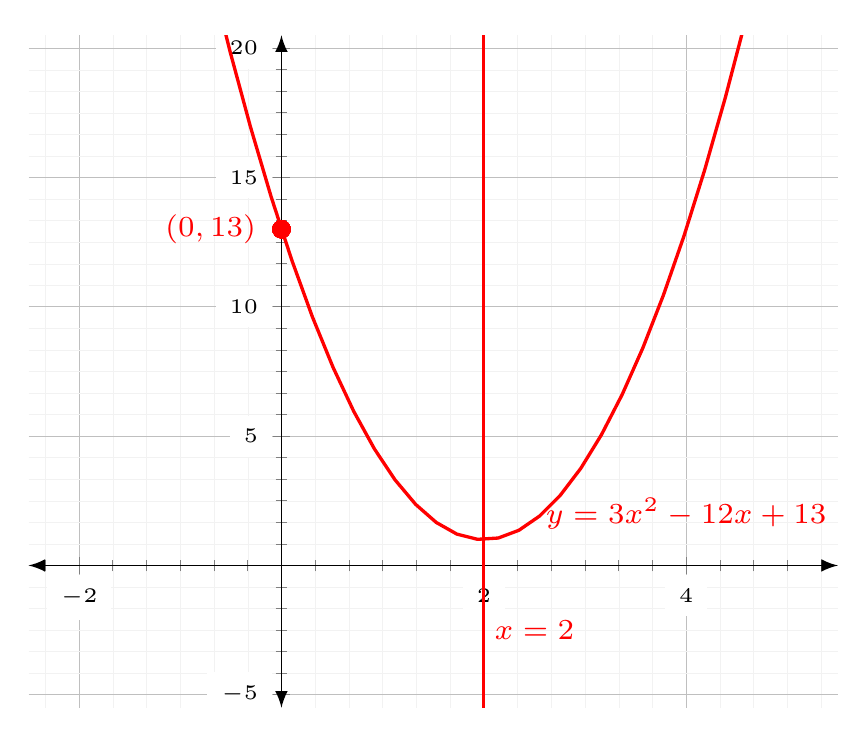
\begin{tikzpicture}[scale=1.5]
				\begin{axis}[xmin=-2,xmax=5,
							 ymin=-5,ymax=20,
   							 grid=both,
    						 grid style={line width=.1pt, draw=gray!10},
    						 major grid style={line width=.2pt,draw=gray!50},
    						 axis lines=middle,
    						 minor tick num=5,
     						 enlargelimits={abs=0.5},
   							 axis line style={latex-latex},
   							 ticklabel style={font=\tiny,fill=white},
   							 xlabel style={at={(ticklabel* cs:1)},anchor=north west},
   							 ylabel style={at={(ticklabel* cs:1)},anchor=south west}]
					\addplot[mark=none, red, thick, samples=50, domain=-5:5]{3*x^2 - 12*x + 13} node at (axis cs:4,2) 
					{\scriptsize $y = 3x^2 - 12x + 13$};
					\addplot[mark=none, red, thick, samples=50, domain=-7:22] (2, x) node at (axis cs:2.5,-2.5) 
					{\scriptsize $x=2$};
					\addplot[only marks, red] (0, 13) node at (axis cs: -0.7, 13) {\scriptsize $(0, 13)$};
				\end{axis}
			\end{tikzpicture}
			\end{figure}
		\end{enumerate}
	\end{ex}
	
	\subsubsection*{Drill Exercises}
	
	\paragraph{}
	\inlinebox{green}{\textbf{1}} Find the real roots of the following polynomials using any method:
	
	\begin{multicols}{2}
		\begin{enumerate}[label=\textbf{(\alph*)}]
			\item $4x - 5$
			\item $x^2 + 4x + 4$
			\item $2x^2 - 4x - 6$
			\item $15x^2 - 45x +26$
			\item $-x^2 + 16x + 19$
			\item $3x^3 + 5x^2 - 4x$
		\end{enumerate}
	\end{multicols}
	
	\paragraph{}
	\inlinebox{yellow}{\textbf{2}} Find the point(s) of intersection (if any) for the following pairs of quadratic equations:
	
	\begin{multicols}{2}
		\begin{enumerate}[label=\textbf{(\alph*)}]
			\item $y = x^2-3x+2$ and $y = x^2+5x-7$
			\item $y = x^2+4x+5$ and $y = -x^2-4x-3$
			\item $y = 3x^2+8x+1$ and $y = -x^2+5x-5$
			\item $y = 5x^2+15x+3$ and $y = -8x^2+4x+6$
			\item $y = x^2$ and $y = 2x^2 + 8$
			\item $y = x^2-6x+9$ and $x = y^2-6y+9$
		\end{enumerate}
	\end{multicols}
	
	\paragraph{}
	\inlinebox{yellow}{\textbf{3}} For each of the following quadratics, use the discriminant to determine the nature of its roots
	(i.e. two distinct real roots, one real root or no real roots):
	
	\begin{multicols}{2}
		\begin{enumerate}[label=\textbf{(\alph*)}]
			\item $3x^2-6x-9$
			\item $2x^2 + 2x + 2$
			\item $2x^2 + 2x + 2$
			\item $y = 5x^2+15x+3$ and $y = -8x^2+4x+6$
			\item $y = x^2$ and $y = 2x^2 + 8$
			\item $y = 4x^2 + (3k-2)x - (k+3)$
		\end{enumerate}
	\end{multicols}
	
	\subsubsection*{Word Problems}	
	
	\paragraph{}
	\inlinebox{green}{\textbf{4}} Consider the quadratic $4x^2 + (3k-2)x - (k+3)$ where $k \in \R$.
	
	\begin{enumerate}[label=\textbf{(\alph*)}]
		\item Determine the range of values of $k$ for which the quadratic has two distinct real roots.
		\item Hence determine the value of $k$ for which the roots are closest together.
	\end{enumerate}
	
	\paragraph{}
	\inlinebox{yellow}{\textbf{5}} For the quadratic $4x^2 - 10x + k$ ($k \in \R$), one root is four times the other root.
	Find the value of $k$.
	
	\paragraph{}
	\inlinebox{yellow}{\textbf{6}} Mahir kicks a football. The height of the football, $h$, can be modeled with respect to its horizontal
	distance, $d$, by the equation $h = d-0.04d^2+0.2$. Assume both $h$ and $d$ are measured in meters.
	Find the maximum height reached by the ball.


	\newpage
	
	\subsection{The binomial theorem}
	
	\paragraph{}
	Consider the expansion of $(a+b)^2$. It should be fairly obvious that this will be $a^2 + 2ab + b^2$. What about $(a+b)^3$?
	With some work, you'll find it is $a^3 + 3a^2b + 3ab^2 + b^3$. For higher integral powers, you will find it becomes harder to
	expand these increasing expressions. But there is an easier way of finding coefficients of each term for higher integral powers of $n$.
	
	\paragraph{}
	First, it is worth looking at what a factorial is:\\
	
	\begin{kp}[The factorial function]
		For $n \in \Z$ where $n \geq 0$, we define $n!$ to be the \textit{factorial} of $n$ given by the function:
		
		$$n! = f(n) = n f(n-1), \quad f(0) = 1$$
		
		or in other words:
		
		$$n! = 1 \cdot 2 \cdot 3 \cdots n \text{ for } n \geq 1 \text{ and } 0! = 1$$
	\end{kp}
	
	\paragraph{}
	For example, $5! = 1 \cdot 2 \cdot 3 \cdot 4 \cdot 5 = 120$.
	Then the binomial theorem is as follows:\\
	
	\begin{kp}[Binomial theorem]
		For $a,b \in \R$ and $n \in \N$
		
		$$(a+b)^n = \sum_{r=0}^n {n \choose r} a^r b^{n-r}$$
		
		Where ${n \choose r}$ is the \textit{binomial coefficient} defined by $\displaystyle {n \choose r} = \dfrac{n!}{r!(n-r)!}$ for
		$0 \leq r \leq n$.
	\end{kp}
	
	\paragraph{}
	You do not need to know the proof, but it is shown below if you are interested:\\
	
	\begin{pf}
		\begin{theorem*}
			For $a,b \in \R$ and $n \in \N$, $\displaystyle (a+b)^n =  \sum_{r=0}^n {n \choose r} a^r b^{n-r}$
		\end{theorem*}
		
		\tcbline
		
		\begin{proof}
			An inductive proof seems best. For more information on how this works, look up \textit{proof by induction}. HL students will
			learn this proof technique later in the course.\\
			
			Let $P(n)$ denote the above statement for $n \in \N$ and consider: $P(0)$:\\
			
			LHS: $(a+b)^0 = 1$\\
			RHS: $\displaystyle \sum_{r=0}^0 {0 \choose r}  a^r b^{-r} = 1 \cdot a^0 b^0 = 1$\\
			
			LHS = RHS, so $P(0)$ is true.\\
			
			Assume $P(k)$ is true for some $k \in \N$: $\displaystyle (a+b)^k = \sum_{r=0}^k {k \choose r} a^r b^{k-r}$\\
			
			Then consider $\displaystyle (a+b)^{k+1} = (a+b) (a+b)^k = (a+b) \sum_{r=0}^k {k \choose r} a^r b^{k-r}$\\
			
			$\displaystyle = \sum_{r=0}^k {k \choose r} a^{r+1} b^{k-r} + \sum_{r=0}^k {k \choose r} a^r b^{k+1-r}$\\
			
			$\displaystyle = \sum_{r=1}^{k+1} {k \choose {r-1}} a^r b^{k+1-r} + \sum_{r=0}^k {k \choose r} a^r b^{k+1-r}$\\
			
			$\displaystyle = \sum_{r=0}^k {k \choose {r-1}} a^r b^{k+1-r} + \sum_{r=0}^{k+1} {k \choose r} a^r b^{k+1-r} 
			- {k \choose {-1}} a^0 b^{k+1} - {k \choose {k+1}} a^{k+1} b^0$\\
			
			$\displaystyle = \sum_{r=0}^k \left({k \choose {r-1}} + {k \choose r}\right) a^r b^{k+1-r}$\\
			
			$\displaystyle = \sum_{r=0}^k {{k+1} \choose r} a^r b^{k+1-r}$\\
			
			Therefore, $P(k+1)$ is true assuming $P(k)$ is true.\\
			
			Hence, $P(n)$ is true for all values of $n \in \N$ by induction.
		\end{proof}
	\end{pf} 
	
	\paragraph{}
	Notice that we had $\displaystyle {k \choose {k+1}}$ and $\displaystyle {k \choose {-1}}$ in the proof.
	These, by convention, both evaluate to zero. To see why, consider:
	
	\paragraph{}
	$\displaystyle {n \choose r} = \dfrac{n!}{r!(n-r)!} = \dfrac{n(n-1)(n-2) \cdots (n - (r-1))}{r(r-1)(r-2) \cdots 1}$
	
	\paragraph{}
	Then $\displaystyle {k \choose {k+1}} = \dfrac{k(k-1)(k-2) \cdots 0}{k(k-1) \cdots 1} = 0$
	
	\paragraph{}
	Similarly $\displaystyle {k \choose {-1}} = {k \choose {k+1}} = 0$ (by symmetry)
	
	\paragraph{}
	The binomial coefficient should be explored further. It seems difficult to generate ${n \choose r}$ for some $n,r \in \N$ by hand, but
	actually it is easy. In fact, you can \textbf{very} easily generate all the coefficients of the expansion of $(a+b)^n$. It is a pattern
	called \textit{Pascal's triangle}:
	
	$$\begin{array}{c}1\\1\quad 1\\1\quad 2\quad 1\\1\quad 3\quad 3\quad 1\\1\quad 4\quad 6\quad 4\quad 1\\1\quad 5\quad 
	10\quad 10\quad 5\quad 1\\1\quad 6\quad 15\quad 20\quad 15\quad 6\quad 1\\1\quad 7\quad 21\quad 35\quad 35\quad 21\quad 
	7\quad 1\\\end{array}$$
	
	\hfill
	
	\paragraph{}
	The above shows Pascal's triangle for $n=0$ to $n=7$, but can be continued. Start the top of the triangle at 1 and then each element
	below is generated at the midpoint of two upper elements by adding them together. 1 is appended on the left and right of each row.
	Notice the third row ($n=2$) gives the coefficients of the expansion of $(a+b)^2 = a^2 + 2ab + b^2$ and similarly the fourth row
	($n=3$) gives the coefficients of the expansion of $(a+b)^3 = a^3 + 3a^2b + 3ab^2 + b^3$. You can verify that this pattern continues
	further. Notice the symmetry as well. The $k$'th term coefficient is the same as that of the $n-k$'th term, which algebraically makes
	sense too.
	
	\paragraph{}
	This pattern comes from the fact that $\displaystyle {n \choose r} = {{n-1} \choose {r-1}} + {{n-1} \choose r}$, which can be verified
	with some algebra. Pascal's triangle comes in handy during a paper 1 exam when you need to quickly obtain binomial coefficients for
	high powers.\\
	
	\stepcounter{excount}
	\begin{ex}
		Find the coefficient of $x^5$ in the expansion ${\left(x-3\right)}^8$.
		
		\hfill
		\tcbline
		\hfill
		
		By the binomial theorem, the $x^5$ term of the expansion will be:\\ 
		
		$\displaystyle {8 \choose 5} x^5 \cdot (-3)^{8-5} = 56 \cdot (-3)^{3} \cdot x^5 = -1512x^5$\\
		
		Hence, the coefficient of $x^5$ is $-1512$.
	\end{ex}
	
	\paragraph{}
	Most of questions you will get in the exam regarding the binomial theorem will be like the one above. They can make some of
	them trickier, though:\\
	
	\stepcounter{excount}
	\begin{ex}
		Find the constant term in the expansion ${\left(1-\dfrac{2}{x}\right)}^5 {\left(x^2+1\right)}^3$.
		
		\hfill
		\tcbline
		\hfill
		
		The above is equivalent to ${\left(1-2x^{-1}\right)}^5 {\left(x^2+1\right)}^3$.\\
		
		The possible powers of $x$ for ${\left(1-2x^{-1}\right)}^5$ are: $0, -1, -2, -3, -4, -5$\\
		The possible powers of $x$ for ${\left(x^2+1\right)}^3$ are: $0, 2, 4, 6$\\
		
		We need to find combinations of power terms which multiply to give $x^0$. These are:
		
		\begin{itemize}
			\item $Ax^0 \cdot Bx^0$
			\item $Ax^{-2} \cdot Bx^2$
			\item $Ax^{-4} \cdot Bx^4$
		\end{itemize}
		
		The constant term for the left expression is $1$\\
		The constant term for the right expression is $1$\\
		The $x^{-2}$ term for the left expression is $\displaystyle {5 \choose 2} (-2)^2 x^{-2}$\\
		The $x^2$ term for the right expression is $\displaystyle {3 \choose 1} x^2$\\
		The $x^{-4}$ term for the left expression is $\displaystyle {5 \choose 4} (-2)^4 x^{-4}$\\
		The $x^2$ term for the right expression is $\displaystyle {3 \choose 2} x^4$\\
		
		The constant term will be the sum of these multiplied combinations:\\
		
		$\displaystyle = 1 \cdot 1 + {5 \choose 2} (-2)^2 x^{-2} \cdot {3 \choose 1} x^2 + {5 \choose 4} (-2)^4 x^{-4} \cdot 
		{3 \choose 2} x^4$\\
		
		$\displaystyle = 1 + 10 \cdot 4 \cdot 3 + 5 \cdot 16 \cdot 3$\\
		
		$\displaystyle = 1 + 120 + 240 = 361$\\
	\end{ex}
	
	\paragraph{}
	By narrowing down term powers which result from multiplication using the binomial theorem, we can avoid performing 
	nasty expansions to obtain specific coefficients. We will look at the \textit{extended binomial theorem} later on, which looks at
	binomial expansions with rational and negative integer powers.


	\subsubsection*{Drill Exercises}	
	
	\paragraph{}
	\inlinebox{green}{\textbf{1}} Use Pascal's triangle (or otherwise) to expand the following:
	
	\begin{multicols}{2}
		\begin{enumerate}[label=\textbf{(\alph*)}]
			\item $(x+1)^4$
			\item $(x+1)^5$
			\item $(x+1)^6$
			\item $(x+1)^{10}$
			\item $(x^2+1)^5$
			\item $(x^3 - 4)^6$
			\item $\left(1 + \dfrac{1}{x}\right)^6$
			\item $\left(4 - \dfrac{2}{5x^2}\right)^9$
		\end{enumerate}	
	\end{multicols}

	\subsubsection*{Word Problems}	
	
	\paragraph{}
	\inlinebox{green}{\textbf{2}} Show that $\displaystyle {n \choose r} = \prod_{k=1}^r \dfrac{n+1 - k}{k}$
	
	\paragraph{}
	\inlinebox{green}{\textbf{3}} Show that $\displaystyle {n \choose r} {r \choose k} = {n \choose k} {{n-k} \choose {r-k}}$
	
	\paragraph{}
	\inlinebox{yellow}{\textbf{4}} Show that $\displaystyle \sum_{r=0}^n {n \choose r}^2 = {{2n} \choose n}$\\ 
	
	\textit{Hint: consider the expansion of $(x+1)^{2n}$ and compare it to the expansion of $((x+1)^n)^2$.}
	
	
	\newpage
	
	\subsection{Polynomial theorems [HL]}
	
	\paragraph{}
	This topic will cover a few major theorems for generic polynomials of one variable. Before looking at these, here's an important
	note:\\
	
	\begin{kp}[Degree of a polynomial]
		The \textit{degree} of a single-variable polynomial $P(x)$ is the highest power of $x$ for which the coefficient is non-zero
		(this is denoted by $\text{deg}(P)$ normally).\\
		
		In general, for $P(x) = a_n x^n + a_{n-1} x^{n-1} + ... + a_1 x + a_0$ where $a_n \neq 0$, $\text{deg}(P) = n$.
	\end{kp}
	
	\paragraph{}
	The first theorem is the \textit{remainder theorem}, which states the following:\\
	
	\begin{pf}
		\begin{theorem*}
			For a polynomial $P(x)$, the remainder when $P(x)$ is divided by $x-r$ is $P(r)$
		\end{theorem*}
		
		\tcbline
		
		\begin{proof}
			This proof uses the \textit{Euclidean Division Theorem}, which will not be proven here (as it isn't directly used in this course).
			You can find the proof in \textbf{Appendix A} on page \pageref*{apA:euc-div}.\\
			
			From this algorithm, there are polynomials $Q(x)$ and $R(x)$ for which $P(x) = (x-r)Q(x) + R(x)$, where
			$R(x)$ is the remainder when $P(x)$ is divided by $x-r$ and $\text{deg}(R) < \text{deg}(g) = 1$. This means $\deg(R) = 0$ and thus 
			$R(x)$ is constant.\\
			
			We have then that $P(r) = R(r) = R(x)$, so $P(r)$ is the remainder when $P(x)$ is divided by $x-r$.
		\end{proof}
	\end{pf} 
	
	\paragraph{}
	The other theorem is the \textit{factor} theorem:\\
	
	\begin{pf}
		\begin{theorem*}
			For a polynomial $P(x) = a_n x^n + a_{n-1} x^{n-1} + ... + a_1 x + a_0$ where $x$ is a variable and $a_0, ..., a_n$ are
			coefficients, $x-r$ is a factor of $P(x)$ if and only if $r$ is a root of $P(x)$.
		\end{theorem*}
		
		\tcbline
		
		\begin{proof}
			$\implies$ Suppose $x-r$ is a factor of $P(x)$. Then\\ $P(x) = (x-r)(b_{n-1} x^{n-1} + ... + b_1 x + b_0)$ for some coefficients 
			$b_0, ..., b_{n-1}$. \\ 
			
			Clearly $P(r) = 0$, so $r$ is a root.\\
			
			$\impliedby$ Now suppose $r$ is a root of $P(x)$, so $P(r) = 0$.\\
			
			By the remainder theorem, there is some polynomial $Q(x)$ and a constant $R$ for which: $P(x) = (x-r)Q(x) + R$.\\
			
			Since $P(r) = 0$, $R = 0$ and therefore $P(x) = (x-r)Q(x)$, which means $x-r$ is a factor of $P(x)$.
		\end{proof}
	\end{pf} 
	
	\paragraph{}
	To summarize:\\
	
	\begin{kp}[Remainder and factor theorems]
		Let $P(x)$ be a polynomial. Then:
		
		\begin{itemize}
			\item When $P(x)$ is divided by $x-r$, the remainder is $P(r)$
			\item $x-r$ is a factor of $P(x)$ if and only if $P(r) = 0$
		\end{itemize}
	\end{kp}
	
	\hfill
	
	\stepcounter{excount}
	\begin{ex}
		Let $f(x) = 3x^4 + 3x^3 - 15x^2 - 9x + 18$
		
		\begin{enumerate}[label=\textbf{(\alph*)}]
			\item Show that $x-1$ is a factor of $f(x)$.
			\item Find the remainder when $f(x)$ is divided by $x+2$
		\end{enumerate}
		
		\hfill
		\tcbline
		\hfill
		
		\begin{enumerate}[label=\textbf{(\alph*)}]
			\item $f(1) = 3 + 3 - 15 - 9 + 18 = 0$, which must imply $x-1$ is a factor (by the factor theorem)
			\item By the remainder theorem, this will be\\ $f(-2) = 3(-2)^4 + 3(-2)^3 - 15(-2)^2 -9(-2) + 18 = 12$
		\end{enumerate}
	\end{ex}
	
	\paragraph{}
	We can also obtain the product and sum of the roots of a polynomial directly in terms of its coefficients. Note that these
	count root multiplicities. For example if $P(x) = (x-r)^2$, $P$ has one root $r$ with multiplicity 2, so $r$ is counted or multiplied
	twice to give a sum of $2r$ and product of $r^2$.\\
	
	\begin{pf}
		\begin{theorem*}
			For a polynomial $P(x) = a_n x^n + a_{n-1} x^{n-1} + ... + a_1 x + a_0$, the sum of the roots, $S_r$, is
			given by:
			
			$$S_r = -\dfrac{a_{n-1}}{a_n}$$
		\end{theorem*}
		
		\tcbline		
		
		\begin{proof}
			Let $\{r_1, ..., r_n\}$ be the roots of the polynomial (there will be exactly $n$ roots in $\C$ including repeated ones). Then the polynomial
			can be written as $P(x) = a_n(x-r_1)(x-r_2)...(x-r_n)$ (by the factor theorem).\\
			
			Expand the factors and notice that the $x^{n-1}$-coefficient is: $-a_n(r_1 + r_2 + ... + r_n)$. Let the sum of the roots
			be denoted by $S_r$. Then the $x^{n-1}$ coefficient is $-a_n S_r$.\\
			
			Equate this coefficient with the original polynomial's coefficient to get: $-a_n S_r = a_{n-1}$\\
			
			This implies, by rearranging, that $S_r = -\dfrac{a_{n-1}}{a_n}$.	
		\end{proof}
	\end{pf}
	
	\begin{pf}
		\begin{theorem*}
			For a polynomial $P(x) = a_n x^n + a_{n-1} x^{n-1} + ... + a_1 x + a_0$, the product of the roots, $P_r$, is
			given by:
			
			$$P_r = \dfrac{(-1)^n a_0}{a_n}$$
		\end{theorem*}
		
		\tcbline		
		
		\begin{proof}
			$P(x) = a_n(x-r_1)(x-r_2)...(x-r_n)$ (by the factor theorem).\\
			
			Expand the factors and notice that the constant term is: $(-1)^n r_1 r_2 ... r_n$. Let the product of the roots
			be denoted by $P_r$. Then the constant term is $a_n (-1)^n P_r$.\\
			
			Equate this term with the original polynomial's constant term to get: $a_n (-1)^n P_r = a_0$\\
			
			This implies, by rearranging, that $P_r = \dfrac{(-1)^n a_0}{a_n}$.	
		\end{proof}
	\end{pf}

	\begin{ex}
		Let $f(x) = x^3 + bx^2 + cx + d$, where $b,c,d \in \R$. $4$ is a root of $f$.
		Given that the sum of the roots is $4$ and the product of the roots is $-8$, find $b$, $c$ and $d$.
		
		\hfill
		\tcbline
		\hfill
		
		$4 = -b \implies b = -4$\\
		
		$-8 = -d \implies d = 8$\\
		
		Finally, $f(4) = 0 = 4^3 - 4^3 + 4c + 8 \implies c + 2 = 0 \implies c = -2$
	\end{ex}
	
	\paragraph{}
	All these theorems covered apply to $\C$ as well. We will look at this in a later chapter.
	
	\subsubsection*{Drill Exercises}
	
	\paragraph{}
	\inlinebox{green}{\textbf{1}} Find the remainders of the following polynomial divisions:
	
	\begin{multicols}{2}
		\begin{enumerate}[label=\textbf{(\alph*)}]
			\item $2$ when divided by $x-4$
			\item $4x+9$ when divided by $x+2$
			\item $2x^2 - x - 6$ when divided by $x-2$\columnbreak
			\item $3x^3 + 3x^2 + 3x + 3$ when divided by $x-5$
			\item $-x^4 + 2x^3 - 3x^2 + 4x$ when divided by $x+1$
			\item $a_n x^n + a_{n-1} x^{n-1} + ... + a_1 x + a_0$ when divided by $x$.
		\end{enumerate}
	\end{multicols}
	
	\paragraph{}
	\inlinebox{yellow}{\textbf{2}} Factorize the following polynomials into linear factors (factors of the form $x-a$) given the additional 
	information provided:
	
	\begin{multicols}{2}
		\begin{enumerate}[label=\textbf{(\alph*)}]
			\item $x^3 - 6x^2 + 11x - 6$ given that $f(1) = 0$
			\item $x^3 + x^2 - 2x - 2$ given that the sum of two of the roots is $0$
			\item $x^3 - 5x^2 - 8x + 48$ given that two of the roots are equal
			\item $x^3 + 3x^2 - x - 3$ given that the roots form an arithmetic sequence with first term $-3$
		\end{enumerate}
	\end{multicols}
	
	\subsubsection*{Word Problems}	
	
	\paragraph{}
	\inlinebox{green}{\textbf{3}} Consider the cubic $6x^3 - 24x^2 + 30x - k$ and let the product and sum of its roots be
	$P_r$ and $S_r$, respectively. Given that $P_r + S_r = 0$, find the value of $k$.
	
	\paragraph{}
	\inlinebox{yellow}{\textbf{4}} The polynomial $x^3 + ax^2 + bx + 12$ is divisible by $x+3$ and $x+2$. Find the values of $a$ and $b$.
	
	\paragraph{}
	\inlinebox{yellow}{\textbf{5}} Let $q(x)$ be a polynomial of degree $n$ and let $S_q$ denote the sum of its roots. 
	Let $r(x) = q(x + k)$ for $k \in \R$.\\
	
	Find an expression for the sum of the roots of $r(x)$, $S_r$, in terms of $S_q$, $k$ and $n$.
	
	\newpage
	
%	\subsection{MOVE TO TAYLOR! The extended binomial theorem [HL]}
%	
%	\paragraph{}
%	This section looks at binomial expansion for fractional and negative integer powers. While this seems a bit strange, there is indeed
%	a catch to this (of sorts). Firstly, the expansion will be an infinite series as opposed to a finite series like with positive integer powers.
%	We will see how this exactly works.
%	
%	\paragraph{}
%	Consider the expression $\sqrt{x+1}$. We wish to expand this using the binomial theorem to express it as a polynomial.
%	Note that $\sqrt{x+1} = (x+1)^{\frac{1}{2}}$, so there is a fractional power which isn't an integer. The binomial theorem
%	states that (for a positive integer $n$):
%	
%	$$(a+b)^n = \sum_{k=0}^n {n \choose k} a^k b^{n-k}$$
%	
%	\paragraph{}
%	Note that $\displaystyle {n \choose k} = \dfrac{n!}{k!(n-k)!} = \dfrac{n(n-1)(n-2) \cdots (n-k+1)}{k!}$. We use this definition of
%	the binomial coefficient and treat $n$ as a rational number (note that $k$ is still an integer). Let's have a look at the expansion again:
%	
%	$$(a+b)^n = \sum_{k=0}^n \dfrac{n(n-1)(n-2) \cdots (n-k+1)}{k!} a^k b^{n-k}$$
%	
%	\paragraph{}
%	Let $n$ be a positive integer and notice that:
%	
%	$${n \choose {n+1}} = \dfrac{n(n-1)(n-2) \cdots (n - (n+1) + 1)}{(n+1)!} = \dfrac{n(n-1)(n-2) \cdots 0}{(n+1)!} = 0$$
%	
%	\paragraph{}
%	We can see that any extra terms after the $n$'th term of the expansion is zero when $n$ is a positive integer. We can hence express:\\
%	
%	$$(a+b)^n = \sum_{k=0}^\infty \dfrac{n(n-1)(n-2) \cdots (n-k+1)}{k!} a^k b^{n-k}$$
%	
%	without any consequence.
%	
%	\paragraph{}
%	When $n$ is either a negative integer or $n \in \Q \setminus \Z$, notice that zero doesn't appear as a term in the binomial coefficient.
%	Hence, we continue the series infinitely. Going back to the expansion of $\sqrt{x+1}$, we have:
%	
%	$$\sqrt{x+1} = \sum_{k=0}^{\infty} \dfrac{\frac{1}{2}(-\frac{1}{2})(-\frac{3}{2}) \cdots (n - k + 1)}{k!} x^k 1^{\frac{1}{2}-k}$$
%	
%	$$= 1 + \dfrac{1}{2}x - \dfrac{1}{4 \cdot 2!}x^2 + \dfrac{3}{8 \cdot 3!}x^3 - \dfrac{15}{16 \cdot 4!}x^4 + ...$$
%	
%	$$= 1 + \dfrac{1}{2}x - \dfrac{1}{8}x^2 + \dfrac{1}{16}x^3 - \dfrac{5}{128}x^4 + ...$$
%	
%	\paragraph{}
%	This is indeed the expansion for $\sqrt{x+1}$. Let's have a look at the expansion of $(x+1)^{-1}$:\\
%	
%	$$(x+1)^{-1} = \sum_{k=0}^{\infty} \dfrac{(-1)(-2)(-3) \cdots (-k)}{k!} x^k$$
%	
%	$$= 1 - x + x^2 - x^3 + x^4 - ...$$
%	
%	\paragraph{}
%	Notice that this is a geometric series with first term $1$ and common ratio $-x$. Hence, the series converges when $|-x| < 1$
%	with sum to infinity: $S_\infty = \dfrac{1}{1-(-x)} = \dfrac{1}{1+x}$, which is our original expression! Now you will notice that this
%	formula will not hold for $|x| \geq 1$. An example is if we set $x=1$. Then $\dfrac{1}{x+1} = \dfrac{1}{2}$, but the expansion
%	gives $1 - 1 + 1 - 1 + 1 - 1 + ...$, which diverges. So it would seem these types of expansions aren't always accurate for all values
%	of $x$.
	
	
	\newpage
	
\section{Functions}
	
	\subsection{Exponents and logarithms}

	\paragraph{}
	This section introduces the concept of exponential and logarithmic functions. Both of these types of functions prove to have
	significance in topics such as analysis and modeling.
	
	\paragraph{}
	An exponential function has the form $f(x) = a^x$. Instead of the variable being raised to the power of a constant like with
	polynomials, an exponential function has a constant raised to the variable. This leads to a much quicker increase or decrease of
	the function (generally) than polynomials have.
	
	\paragraph{}
	A logarithmic function has the form $g(x) = \log_a(x)$ and is the \textbf{inverse} of an exponential function. Hence, you can think about 
	logarithmic functions as a reflection of a corresponding exponential function on the line $y=x$. We also have that $a^{\log_a(x)} = 
	\log_a(a^x) = x$.
	
	\paragraph{}
	We will come across the constant $\e$ often. This section will introduce the usefulness of $\e$ (to some extent).
	
	\paragraph{}
	An \textit{exponent} is the part of a number which denotes the power some number is raised by. For the expression $a^n$, we
	say that $a$ is the \textit{base} and $n$ is the \textit{exponent} and we read this number as ``$a$ to the power of $n$'' or
	more simply ``$a$ to the $n$''. Before jumping into the analysis and use of exponential functions, it would be useful to review the laws 
	of exponents. They are as follows:
	
	\begin{kp}[Laws of exponents]
		Let $a, b, m, n \in \R$. Then:
		
		\begin{itemize}
			\item $a^m \cdot a^n = a^{m+n}$ (multiplication law)
			\item $\dfrac{a^m}{a^n} = a^{m-n}$ (division law)
			\item ${(a^m)}^n = a^{mn}$ (exponentiation law)
			\item $(ab)^m = a^m b^m$ (distribution law)
			\item $a^0 = 1$ if $a \neq 0$
			\item $0^m = 0$ if $m \neq 0$
			\item $0^0$ is \textbf{undefined}
		\end{itemize}
	\end{kp}
	
	\paragraph{}
	It may be useful to know why $0^0$ is undefined. It's because we can obtain different values from it depending on how we
	approach it. Consider the two graphs below:
	
	\begin{figure}[H]
			\centering
			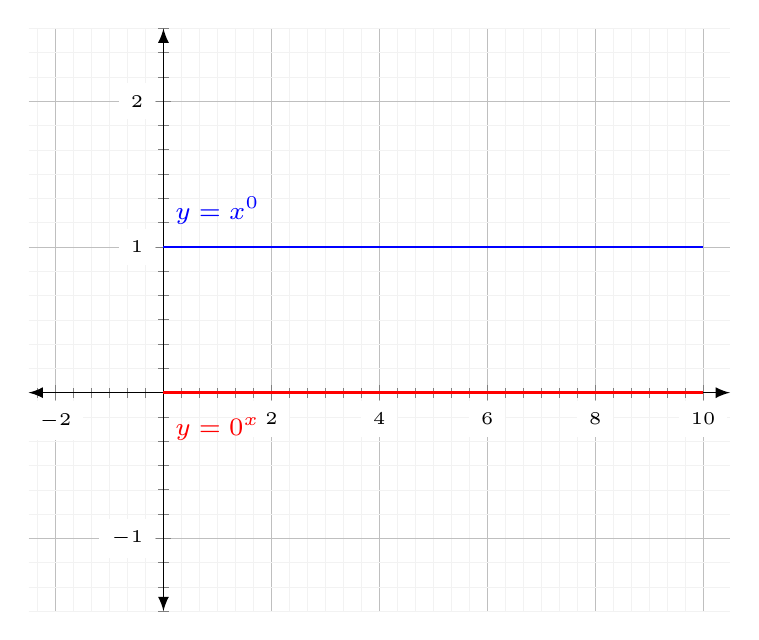
\begin{tikzpicture}[scale=1.3]
				\begin{axis}[xmin=-2,xmax=10,
							 ymin=-1,ymax=2,
   							 grid=both,
    						 grid style={line width=.1pt, draw=gray!10},
    						 major grid style={line width=.2pt,draw=gray!50},
    						 axis lines=middle,
    						 minor tick num=5,
     						 enlargelimits={abs=0.5},
   							 axis line style={latex-latex},
   							 ticklabel style={font=\tiny,fill=white},
   							 xlabel style={at={(ticklabel* cs:1)},anchor=north west},
   							 ylabel style={at={(ticklabel* cs:1)},anchor=south west}]
					\addplot[mark=none, red, thick, samples=50, domain=0:10]{0} node at (axis cs:1,-0.25) 
					{\scriptsize $y = 0^x$};
					\addplot[mark=none, blue, thick, samples=50, domain=0:10]{1} node at (axis cs:1,1.25) 
					{\scriptsize $y = x^0$};
				\end{axis}
			\end{tikzpicture}
		\end{figure}

	\paragraph{}
	It can be seen that two different functions approach two distinct values of $0^0$. Hence, $0^0$ is undefined (or indeterminate).
	
	\paragraph{}
	We can also use the laws of exponents to recognize that $\sqrt[n]{a} = a^{\frac{1}{n}}$. For example, we can write
	$\sqrt{2} = 2^{\frac{1}{2}}$. Converting roots to this form can help make exponential calculations easier to perform.\\
	
	\stepcounter{excount}
	\begin{ex}
		Express the following values in the form $a^n$ where $a, n \in \Q$
		
		\begin{enumerate}[label=\textbf{(\alph*)}]
			\item $4 \cdot 4^5$
			\item $2 \cdot 8^2$
			\item $3^8 \cdot 9^3$
			\item $\sqrt{2} \cdot 4$
		\end{enumerate}
		
		\tcbline
		
		\begin{enumerate}[label=\textbf{(\alph*)}]
			\item $4 \cdot 4^5 = 4^{1+5} = 4^6$
			\item $2 \cdot 8^2 = 2 \cdot (2^3)^2 = 2 \cdot 2^{3 \cdot 2} = 2^{1+6} = 2^7$
			\item $3^8 \cdot 9^3 = 3^8 \cdot (3^2)^3 = 3^{8+6} = 3^{14}$
			\item $\sqrt{2} \cdot 4 = 2^{\frac{1}{2}} \cdot 2^2 = 2^{\frac{1}{2} + 2} = 2^{\frac{5}{2}}$
		\end{enumerate}
	\end{ex}
	
	\paragraph{}
	It may be useful to know the general shape of the graph of $f(x) = a^x$ for $a > 0$ ($a \neq 1$). Before we plot it, it may be worth
	determining some points:
	
	\begin{itemize}
		\item $f(0) = a^0 = 1$
		\item $f(1) = a^1 = a$
		\item $\displaystyle \lim_{x \to \infty} f(x) = \infty$ if $a>1$
		\item $\displaystyle \lim_{x \to -\infty} f(x) = 0$ if $a>1$
		\item $\displaystyle \lim_{x \to \infty} f(x) = 0$ if $a<1$
		\item $\displaystyle \lim_{x \to -\infty} f(x) = \infty$ if $a<1$
	\end{itemize}
	
	\paragraph{}
	The last four points refer to the function behavior when $x$ approaches infinity (positive or negative) depending on the
	value of $a$. If you have read the section on geometric sequences already, you should be familiar with this type of behavior.
	Of course if $a = 1$, $f(x) = 1$ for all values of $x$.\\

	\begin{figure}[H]
			\centering
			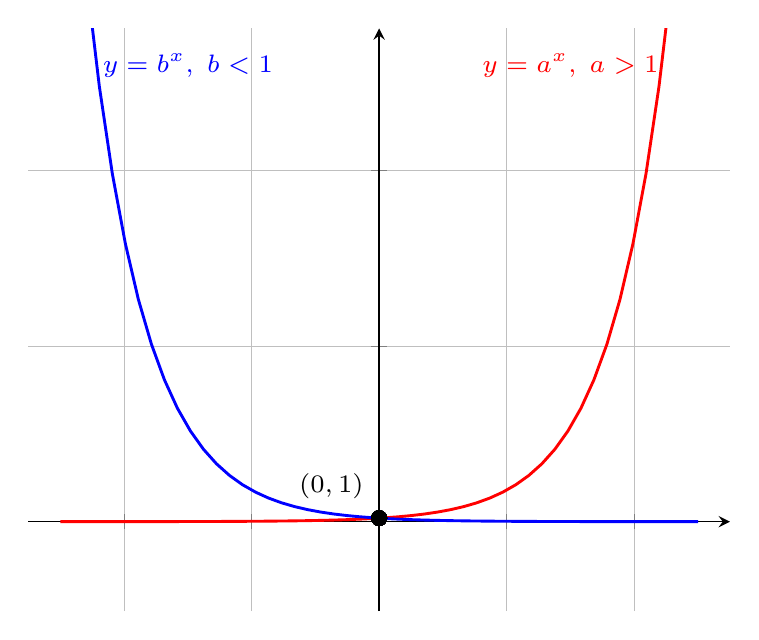
\begin{tikzpicture}[scale=1.3]
				\begin{axis}[xmin=-5,xmax=5,
							 ymin=-25,ymax=140,
   							 grid=both,
    						 grid style={line width=.1pt, draw=gray!10},
    						 major grid style={line width=.2pt,draw=gray!50},
    						 axis lines=middle,
     						 enlargelimits={abs=0.5},
     						 xticklabels={,,},
     						 yticklabels={,,}]
					\addplot[mark=none, red, thick, samples=50, domain=-5:5]{3^x} node at (axis cs:3,130) 
					{\scriptsize $y = a^x, \; a > 1$};
					\addplot[only marks, black] (0, 1) node at (axis cs: -0.75, 10) {\scriptsize $(0, 1)$};
					\addplot[mark=none, blue, thick, samples=50, domain=-5:5]{3^(-x)} node at (axis cs:-3,130) 
					{\scriptsize $y = b^x, \; b < 1$};
				\end{axis}
			\end{tikzpicture}
	\end{figure}
	
	\paragraph{}
	Notice that no such value $x$ in $\R$ gives $a^x \leqslant 0$ for any value of $a$ in $\R$. $a^x$ will always be positive.

	\paragraph{}
	It is common to use the base $\e$ for a generic exponential function (i.e. $f(x) = \e^x$). $\e$ is a very special
	number in mathematics; probably the most important constant. As for why that is the case, later chapters will shed more light
	on this. However, you will be working with $\e^x$ very frequently in the course. Note that $\e > 1$, so the shape of $\e^x$
	can be easily deduced using the facts from above.\\

	\begin{fr}[Expressing \boldmath $\e^x$ as a power series]
		While values such as $2^3$ and $5^6$ are intuitive to evaluate, the same can't be said for $\e^x$. This is especially
		difficult since $\e$ is irrational.\\
	
		We need to find a way to obtain approximations of $\e^x$ in terms of $x$. Luckily, there are ways of doing so. For instance,
		we know that $\displaystyle \lim_{n \to \infty} \left(1+\dfrac{1}{n}\right)^n = \e$, so larger values of $n$ will mean closer rational
		approximations to $\e$, which we can take to the power of some $x$. However, this is very tedious to do by hand.\\
		
		An easier way to find an approximation for $\e^x$ in terms of $x$ is to perform a \textit{binomial expansion} on the limit
		definition of $\e^x$ (which we will prove later on in the course):
		
		$$\e^x = \lim_{n \to \infty} \left(1+\dfrac{x}{n}\right)^n$$
		
		\hfill
		
		Notice that for $x=1$, we obtain $\e^1 = \e$, as per the definition of $\e$. Additionally, $x=0$ yields $\e^0 = 1$, which also makes
		sense.\\
		
		If we expand this expression using the binomial theorem:
		
		$$\e^x = \lim_{n \to \infty} 1 + {n \choose 1} \dfrac{x}{n} + {n \choose 2} \dfrac{x^2}{n^2} + {n \choose 3} \dfrac{x^3}{n^3} + ...$$
		
		$$= \lim_{n \to \infty} 1 + \dfrac{n}{n} x + \dfrac{n(n-1)}{n^2} \dfrac{x^2}{2!} + \dfrac{n(n-1)(n-2)}{n^3} \dfrac{x^3}{3!} + ...$$
		
		$$= 1 + x + \dfrac{x^2}{2!} + \dfrac{x^3}{3!} + ...$$
		
		$$= \sum_{k=0}^{\infty} \dfrac{x^k}{k!}$$
		
		\hfill
		
		We have expressed $\e^x$ as an infinite sum of powers of $x$. Note that this is \textbf{not} a polynomial; a polynomial must have a 
		finite degree. Instead, this is called a \textbf{power series}. By choosing a good-enough $k$ to stop our terms 
		at, we can approximate $\e^x$ quite well. For larger or smaller (negative) values of $x$, you can see that the approximation becomes 
		less accurate.
	\end{fr}
	
	\paragraph{}
	As stated, a logarithm function is an inverse for a corresponding exponential function. The general form is $\log_a(x)$ (read as
	``log to base $a$ of $x$''), where $a$ is the base of its corresponding exponential function. It is such that if $y = a^x$, then 
	$x = \log_a(y)$. In other words, $\log$ can be used to obtain the exponential part of an expression of the form $a^x$. That being said, 
	$a^{\log_a(x)} = x$ and similarly $\log_a(a^x) = x$.
	
	\paragraph{}
	Just as exponential functions have algebraic laws, logarithms do as well:\\
	
	\begin{kp}[Laws of logarithms]
		Let $a, b x, y \in \R^+$ where $a, b \neq 1$ and let $p \in \R$. Then:
		
		\begin{itemize}
			\item $\log_a(xy) = \log_a(x) + \log_a(y)$ (multiplication law)
			\item $ \log_a\left(\dfrac{x}{y}\right) = \log_a(x) - \log_a(y)$ (division law)
			\item $\log_a(x^p) = p \log_a(x)$ (exponentiation law)
			\item $\log_a(x) = \dfrac{\log_b(x)}{\log_b(a)}$ (change of base law)
			\item $\log_a(a) = 1$
			\item $\log_a(1) = 0$
		\end{itemize}
	\end{kp}
	
	\paragraph{}
	These laws follow from the exponential laws and can be proven using them.\\
	
	\stepcounter{excount}
	\begin{ex}
		Solve the equation $5^x = 125$
		
		\hfill
		\tcbline
		\hfill
		
		If $y = a^x$, then $x = \log_a(y)$. Hence, $x = \log_5(125)$. We are looking for a power of $5$ which gives $125$.\\
		
		Intuitively (or using a calculator), this will be $x = 3$. 
	\end{ex}
	
	\paragraph{}
	Since $\e^x$ is used a lot, $\ln$ denotes logarithms to base $\e$ for brevity (i.e. $\log_{\e}(x) = \ln(x)$). It is also common to
	write $\log_a(x)$ as $\dfrac{\ln(x)}{\ln(a)}$ (using the change of base rule) for consistency. Here is a plot of $y = \ln(x)$ 
	on a graph:\\
	
	\begin{figure}[H]
			\centering
			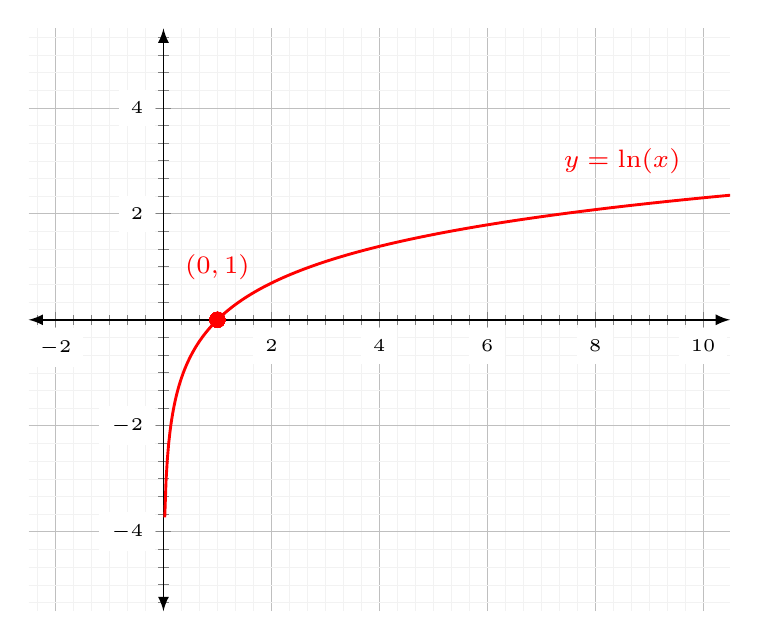
\begin{tikzpicture}[scale=1.3]
				\begin{axis}[xmin=-2,xmax=10,
							 ymin=-5,ymax=5,
   							 grid=both,
    						 grid style={line width=.1pt, draw=gray!10},
    						 major grid style={line width=.2pt,draw=gray!50},
    						 axis lines=middle,
    						 minor tick num=5,
     						 enlargelimits={abs=0.5},
   							 axis line style={latex-latex},
   							 ticklabel style={font=\tiny,fill=white},
   							 xlabel style={at={(ticklabel* cs:1)},anchor=north west},
   							 ylabel style={at={(ticklabel* cs:1)},anchor=south west}]
					\addplot[mark=none, red, thick, samples=500, domain=0:12]{ln(x)} node at (axis cs:8.5,3) 
					{\scriptsize $y = \ln(x)$};
					\addplot[only marks, red] (1, 0) node at (axis cs: 1, 1) {\scriptsize $(0, 1)$};
				\end{axis}
			\end{tikzpicture}
	\end{figure}
	
	\paragraph{}
	Graphs of generic logarithms of the form $\log_a(x)$ will look similar to the above, except for when $0< a < 1$. Remember that
	$y = \log_a(x)$ is just a reflection of $y = a^x$ on the line $y=x$. While it doesn't look like it, note that $\ln(x)$ approaches
	infinity as $x$ does; just very slowly. This is evident from the exponential function.\\
	
	\stepcounter{excount}
	\begin{ex}
		Solve the equation $\e^{2x} - 4\e^x - 1 = 0$ for $x \in \R$, giving your answer(s) in exact form.
		
		\hfill
		\tcbline
		\hfill
		
		Notice that $\e^{2x} = (\e^x)^2$ and substitute $y = \e^x$ to obtain $y^2 - 4y - 1 = 0$. By substituting a common expression
		for a variable, we have converted the equation to a recognizable form; in this case, a quadratic. We just have to make sure our
		final answer is $x$ and not $y$.\\
		
		$y^2 - 4y - 1 = (y-2)^2 - 1 - 4 = 0$\\
		$(y-2)^2 = 5 \implies y-2 = \pm \sqrt{5} \implies y = 2 \pm \sqrt{5}$\\
		
		Then back-substitute $y = \e^x$:\\
		$\e^x = 2 \pm \sqrt{5}$ so $\e^x = 2+\sqrt{5}$ or $2 - \sqrt{5}$.\\
		
		However, notice that $2-\sqrt{5} < 2 - \sqrt{4} = 2 - 2 = 0$ and $\e^x$ can't be negative for any real value $x$.\\
		
		Hence, $\e^x = 2 + \sqrt{5}$ is the only solution, so $x = \ln(2+\sqrt{5})$
	\end{ex}
	
	\paragraph{}
	These types of questions can appear frequently. With a GDC, it will be easier. But by hand, it will require some intuition. You will
	see more of these variable substitution questions later on.
	
	\subsubsection*{Drill Exercises}
	
	\paragraph{}
	\inlinebox{green}{\textbf{1}} Solve the following equations, giving your answers in exact, simplest form:\\
	\textit{Note: $\ln^p(x)$ means $(\ln(x))^p$}	
	
	\begin{multicols}{2}
		\begin{enumerate}[label=\textbf{(\alph*)}]
			\item $5^{x^2} \cdot 4^x = 2$ 
			\item $3^x + 9^x = 4$
			\item $\ln^2(x) + \ln(x) - 1 = 0$
			\item $\log_{x^2}(3) = 3$ (be careful here)
			\item $\ln(\ln^{2}(x)) = 0$
			\item $x^x = x^2$
		\end{enumerate}
	\end{multicols}
	
	\paragraph{}
	\inlinebox{green}{\textbf{2}} Find all solutions to the following equations using a GDC or otherwise.
	Give your answers to at least 3 s.f. where appropriate:
	
	\begin{multicols}{2}
		\begin{enumerate}[label=\textbf{(\alph*)}]
			\item $3^x = x^3$ 
			\item $\e^x = x^2 + 3x + 1$
			\item $\ln(x) + \e^x = 3^{\ln(x)}$
			\item $\dfrac{\e^x - \e^{-x}}{2} = x^5-x^4+x^3-x^2+x+\dfrac{1}{10}$
			\item $\sqrt[x]{x} = x^{\e x}$
			\item $\sqrt{x^x} = x!$ (you may find Desmos particularly useful for this one)
		\end{enumerate}
	\end{multicols}
	
	\hfill
	
	\subsubsection*{Word Problems}
	
	\paragraph{}
	\inlinebox{gray!30}{\textbf{3}} We have seen that $\displaystyle \lim_{n \to \infty} \left(1+\dfrac{x}{n}\right)^n = \e^x$.\\
	Prove that $\displaystyle \lim_{h \to 0} \dfrac{x^h - 1}{h} = \ln(x)$
	
	\hfill
	
	\subsection{Properties of functions}
	
	\paragraph{}
	As the title says, this section looks at properties of functions. In particular, we look at what it means to be a function, the domain, codomain
	and range of a function, function composition, inverse functions and function parity.
	
	\paragraph{}
	Let $f : X \to Y$. This notation says ``let $f$ be a function which maps the set $X$ to the set $Y$''. What this means is $f$ takes any value
	$x$ in the set $X$ and \textit{maps} it to \textbf{exactly one} value $y$ in $Y$. We write $f(x) = y$ to mean $f$ maps $x$ to $y$. 
	Alternatively, we can write $x \mapsto f(x)$ (for example, $f : x \mapsto x^2$ is the same as writing $f(x) = x^2$).
	This notation $f : X \to Y$ tells us the first condition which a function must satisfy: it must
	map each value in $A$ to \textbf{only one} value in $B$. This may seem intuitive enough, but it's important to be aware of this. The reason
	for why this is so is because it's natural to define an equation $y = f(x)$ for graphing. This means each value of $x$ on the $x$-axis is mapped
	to a corresponding value $y = f(x)$ on the $y$-axis. But such equations may not be functions. 

	\paragraph{}	
	For instance, consider the equation $y^2 = 1-x^2$ for $(x,y) \in \R^2$. This equation when graphed will give a unit circle centered at the 
	origin. If we try to
	solve for $y$, we can see that $y = \pm \sqrt{1-x^2}$; two possible values. If we make a choice of $+$ or $-$ and write $y = f(x) = 
	\sqrt{1-x^2}$ or $y = f(x) = -\sqrt{1-x^2}$, we will lose half of the graph (the function will only plot half the circle). We call an equation
	such as $y^2 = 1-x^2$ a \textbf{relation}, but not a function. Given a function $f(x)$, setting $y=f(x)$ gives a relations, but not all relations
	give functions.\\
	
	\begin{kp}[Relations]
		A relation on two sets $X$ and $Y$ is a collection of ordered pairs $(x,y) \in X \times Y$ satisfying a certain property $P(x,y)$.
		We say $x$ is \textit{related to} $y$ if and only if $P(x,y)$ is true.\\
		
		For example, we can set $X = Y = \R$ and define $P(x,y): x^2+y^2=1$. Then we have that $x$ and $y$ are related if and only if
		$y^2 = 1-x^2$. It's easy to verify that the set of solutions $(x,y) \in \R^2$ to the equation gives the set of values satisfying the relation.
	\end{kp}
	
	\paragraph{}
	An easy way to check if a graph represents a function plot $y = f(x)$ is to verify that every vertical line passing through the plane intersects
	no more than 1 point on the graph. 
	
	\paragraph{}
	We actually have names for the sets $X$ and $Y$ in relation to a function $f$.\\
	
	\begin{kp}[Domain, codomain and range]
		For $f : X \to Y$ a function, we say:
		\begin{itemize}
			\item $X$ is the \textbf{domain} of $f$
			\item $Y$ is the \textbf{codomain} of $f$
			\item $f(X) = \{ y \in Y \; \vert \; \text{there is some } x \in X \text{ such that } f(x) = y \}$
			is the \textbf{range} of $f$
		\end{itemize}
	\end{kp}
	
	\paragraph{}
	The one which stands out is the \textbf{range}. The range describes the \textit{subset} of the codomain of values which $f$ is able to
	reach with the given domain $X$. For example, we can define $f : \R \to \R$ by $f(x) = x^2$. It's clear that the domain and codomain of $f$ is
	$\R$, but the range of $f$ is \textbf{not} $\R$ because no negative values of $\R$ can be reached by $f$ given that its domain is $\R$.
	We say that the range is $f(\R) = [0,\infty) \subseteq \R$ or equivalently $f(\R) = \{ y \in \R \; \vert \; y \geqslant 0 \}$. Note that
	the codomain of a function can be chosen to be any superset of the range of the function (or the range itself, of course).
	
	\paragraph{}
	Another point to make is a function must map \textbf{all} values in its domain to some value in the codomain. For example, we can't define
	$g : \R \to \R$ by $g(x) = \sqrt{x}$, because $g(x) \not\in \R$ for any $x < 0$. We would need to write $g : [0,\infty) \to \R$, then it
	would make sense.\\
	
	\stepcounter{excount}
	\begin{ex}
		Write down the domain and range of the following functions:
		
		\begin{itemize}
			\item $f(x) = \e^x$ with codomain $\R$
			\item $g(x) = \ln(x)$ with codomain $\R$
			\item $h(x) = \sqrt[3]{x}$ with codomain $\R$
		\end{itemize}
		
		\tcbline
		\hfill
		
		\begin{itemize}
			\item $f(x) = \e^x$ can map any $x \in \R$ to $\R$, but $\e^x > 0$ for all $x \in \R$. So the domain is $\R$ and the range
			is $\R^+$.
			\item $g(x) = \ln(x)$ maps to $\R$ only when $x > 0$, so the domain is $\R$. It's clear that $\ln(\R^+) = \R$, since we can 
			choose any $y \in \R$ and use $x = \e^y \in \R^+$ to give $\ln(x) = y$ so the range is $\R$.
			\item $h(x) = \sqrt[3]{x}$ is defined on all of $\R$ and maps any value in $\R$ to a value in $\R$. Moreover, given any $y \in \R$, we
			can choose $x = y^3$ to give $h(x) = y$. So the domain and range are both $\R$.
		\end{itemize}
	\end{ex}
	
	\paragraph{}
	The preceding exercise specified that the codomain for each provided function. This is because if the codomain was larger, the corresponding
	domain and range would be different. For example if we chose $\C$ to be the codomain for $f(x) = \e^x$ and $g(x) = \ln(x)$, the range of
	$f$ and the domain of $g$ would both be $\C \setminus \{0\}$ (which includes $\R \setminus \{0\}$). It's not necessary to make this 
	specification given the context of functions mapping reals to reals, but one should nonetheless be aware of this fact.
	
	\paragraph{}
	On page \pageref*{fr:countability}, we looked at the concept of injective, surjective and bijective functions as part of a further reading section.
	We formalize it here:\\
	
	\begin{kp}[Injective, surjective and bijective functions]
		Let $f : X \to Y$ be a function. We say:
		\begin{itemize}
			\item $f$ is \textbf{injective} (\textbf{one-to-one}) when for every $x_1, x_2 \in X$, $f(x_1) = f(x_2) \implies x_1 = x_2$
			\item $f$ is \textbf{surjective} (\textbf{onto}) when for every $y \in X$, we can find some $x \in X$ for which $f(x) = y$
			\item $f$ is \textbf{bijective} when it is both injective and surjective.
		\end{itemize}
	\end{kp}
	
	\paragraph{}
	Here are some examples for $f : \R \to \R$:
	
	\begin{itemize}
		\item $f(x) = \e^x$ is injective but not surjective
		\item $f(x) = x^3 + 2x^2$ is surjective but not injective
		\item $f(x) = x^3 + 2x$ is both injective and surjective
		\item $f(x) = x^2$ is neither injective nor surjective
	\end{itemize}
	
	\paragraph{}
	It's important to know that the codomain of a function determines whether or not a function is surjective. Certainly if a function's codomain
	is the range itself, the function will be surjective (in fact, this is the definition of surjectivity). Also the domain of a function determines whether 
	or not a function is injective or surjective. One can, for example, restrict $f(x) = x^2$ to the domain $[0,\infty)$ and it's clear that the function
	will be injective.
	
	\paragraph{}
	Another important topic is the composition of functions. This is where, given two function $f$ and $g$, we may define a new function
	$h(x) = f(g(x))$ or $h(x) = g(f(x))$ \textbf{if permitted}.\\
	
	\begin{kp}[Function composition]
		Define $f : W \to X$ and $g : Y \to Z$. If $f(W) \subseteq Y$, then we can define a function $h : W \to Z$ by
		$h(w) = g(f(w))$. We write $h = g \circ f$.\\
		
		It's easy to see that if $f : X \to Y$ and $g : Y \to Z$, we can always define $h = g \circ f$ because $f(X) \subseteq Y$ (the range of
		$f$ is contained in the domain of $g$).
	\end{kp}
	
	\paragraph{}
	Define $f : \R \to \R$ by $f(x) = \e^x$ and $g : \R \to \R$ by $x^2$. We have $f(\R) = \R^+$ and $g(\R) = [0,\infty)$, both contained
	in the domain of $f$ and $g$. Thus we can define $h = g \circ f : \R \to \R$ and $k = f \circ g : \R \to \R$. We have that
	$h(x) = \e^{2x}$ and $k(x) = \e^{x^2}$. They clearly aren't the same function, which shows $\circ$ isn't necessarily a commutative operation.
	That is, $f \circ g = g \circ f$ doesn't always hold.\\
	
	\stepcounter{excount}
	\begin{ex}
		Let $f(x) = \sqrt{x}$ and $g(x) = -x^2 + 4kx - 3k^2$ be real functions with $k \neq 0$. Find the domain and range of $f \circ g$ in terms of 
		$k$.
		
		\hfill
		\tcbline
		\hfill
		
		We need to find all $x$ such that $g(x) \geqslant 0$. Observe that $g(x) = -(x^2 - 4kx + 3k^2) = -(x-3k)(x-k)$, so the roots of $g$ are
		$k$ and $3k$. Also, the $x^2$ coefficient of $g$ is negative. Thus we have that $g(x) \geqslant 0$ on the interval $[k, 3k]$, which
		means the domain of $f \circ g$ must be $[k, 3k]$ to be defined.\\
		
		Next, we can see that $g(x) = -(x^2 - 4kx + 3k^2) = -[(x-2k)^2 + 3k^2 - 4k^2] = -(x-2k)^2 + k^2$. Thus the vertex of $g$ is the point
		$(2k, k^2)$, with $k^2 > 0$. This means $g([k, 3k]) = [0,k^2]$. Then $(f \circ g)([k, 3k]) = f([0, k^2]) = [0, |k|]$, so the range of
		$f \circ g$ is $[0, |k|]$.
	\end{ex}
	
	\paragraph{}
	We know that function composition isn't commutative.
	Define $f(x) = x^2$ and $g(x) = \sqrt{x}$. We have that $f : \R \to \R$ with $f(\R) = [0,\infty)$ and $g : [0,\infty) \to \R$
	with $g([0,\infty) ) = [0,\infty)$. We can see that $f(\R)$ is exactly the domain of $g$, which means
	the function $h : \R \to [0,\infty)$ given by $h = g \circ f$ is well-defined. Indeed, we have $h(x) = \sqrt{x^2} = |x|$.
	Conversely we observe that $g([0,\infty))$ is contained in the domain of $f$, but isn't exactly the domain itself.
	This is fine when it comes to defining $k : [0,\infty) \to [0,\infty)$ by $k(x) = (\sqrt{x})^2 = x$. Although $h$ and $k$ have
	the same range, it's clear that they aren't the same function (they have different domains). But you've probably have noticed that there's 
	something special with the particular functions chosen.
	
	\paragraph{}
	If we're given $x^2 \in \R$, we can get back $x$ by taking the square root of $x^2$, but this may yield two possible results. For example
	if $x^2 = 4$, we have $x = 2$ or $x = -2$ as possible values. We can, however, find $x$ given $\sqrt{x} \in [0,\infty)$ by
	squaring the root. That is if $\sqrt{x} = 4$, we have $x = 16$; and this is the only value of $x$ for which $\sqrt{x} = 4$.
	This brings us to the concept of \textbf{identity} and \textbf{inverse} of functions.\\
	
	\begin{kp}[Identity function]
		We call the function $I_X : X \to X$ defined by $I_X(x) = x$ the \textbf{identity function} on $X$. Moreover for any $f : X \to Y$, we have 
		$f \circ I_X = I_Y \circ f$.
	\end{kp} 
	
	\paragraph{}
	It can be seen that an identity depends on the set on which its defined. For instance if we take $f(x) = x^2$ and $g(x) = \sqrt{x}$
	with $f : \R \to [0,\infty)$ and $g : [0,\infty) \to \R$, it's clear that $f \circ g = I_{[0,\infty)}$ (note that we've changed
	the codomain of $f$). We say that $f$ is a \textbf{left inverse} of $g$ which this happens, or equivalently that $g$ is a \textbf{right inverse} 
	of $f$.\\
	
	\begin{kp}[Left and right inverses]
		Let $f : X \to Y$. A \textbf{left inverse} of $f$ is a function $g : Y \to X$ satisfying $g \circ f = I_X$. A \textbf{right inverse} of $f$ is
		a function $h : Y \to X$ satisfying $f \circ h = I_Y$.\\
		
		We say a function is \textbf{left-invertible} when it has a left inverse and is \textbf{right-invertible} when it has a right inverse.
	\end{kp} 
	
	\paragraph{}
	For the same $f$ and $g$, we can see that $g$ isn't a left inverse of $f$. That is, $g \circ f \neq I_{\R}$; it's easy to see because we've
	established that $(g \circ f)(x) = |x| \neq x$ on $\R$. Thus, $f(x) = x^2$ is not left-invertible. If we restrict the domain of $f$ to
	$[0,\infty)$ however, $g$ \textit{would be} a left-inverse, with $g \circ f = I_{[0,\infty)}$.
	
	\paragraph{}
	Now consider $f : \R \to \R$ and $g : \R^+ \to R$ defined by $f(x) = \e^x$ and $g(x) = \ln(x)$. It's apparent that $f \circ g : \R^+ \to \R$
	is $\e^{\ln(x)} = x$, which means $f \circ g = I_{\R^+}$. You probably have noticed that the codomain
	of $f$ isn't $\R^+$ though. However, we know that $f(\R) = \R^+ \subseteq \R$, so we can always restrict the codomain of $f$ to $\R^+$
	if we want. So by making $f : \R \to \R^+$, we can satisfy the inverse requirement and say that $g$ is a right inverse of $f$.
	We typically aren't picky about this, though. As long as the range of $f$ is the domain of $g$, we can say that $f : \R \to \R$
	has a right inverse $g : \R^+ \to \R$.
	We can also see that $(g \circ f)(x) = \ln(\e^x) = x$, so $g \circ f = I_{\R}$. Therefore, $g$ is also a left inverse of $f$. When a function
	has a left inverse \textbf{and} a right inverse, we say the function is \textbf{invertible}.\\
	
	\begin{kp}[Invertible functions]
		A function $f : X \to Y$ is \textbf{invertible} when $f$ has both a left inverse $g : Y \to X$ and a right inverse $h : Y \to X$.
		If a function is invertible, we have that $g = h$ and say that $g$ (or $h$) is the \textbf{inverse} of $f$, denoted $f^{-1}$.
	\end{kp}
	
	\paragraph{}
	So for $f : \R \to \R^+$ given by $f(x) = \e^x$, we have $f^{-1}(x) = \ln(x)$ is the inverse (which can be applied to either the left side
	or the right side of $f$ via composition). We also have another property:\\
	
	\begin{pf}
		\label{fun-prop-ex}
		\begin{theorem*}
			Let $f : X \to Y$ be a function. Then:
			\begin{itemize}
				\item $f$ has a left inverse if and only if $f$ is injective (one-to-one)
				\item $f$ has a right inverse if and only if $f$ is surjective (onto)
				\item $f$ invertible if and only if $f$ is bijective (one-to-one and onto)
			\end{itemize}
		\end{theorem*}
		
		\tcbline
		
		\begin{proof}
			Exercise.
		\end{proof}
	\end{pf}
	
	\hfill
	
	\stepcounter{excount}
	\begin{ex}
		Let $f : [k, \infty) \to \R$ be defined by $f(x) = x^2+3x+4$. Find the least value of $k$ for which $f$ is invertible and find
		$f^{-1}$.
		
		\hfill
		\tcbline
		\hfill
		
		We need $f$ to be such that it's left inverse and right inverse exist and are (consequently) the same. If $f$ is to have a left inverse
		$g$, we need to make sure $f$ is one-to-one on $[k, \infty)$ (by the preceding theorem). Hence, $k$ must at least be the $x$-coordinate
		of the vertex of $f$. We observe that:
		\[ f(x) = (x+\tfrac{3}{2})^2 + 4 - \tfrac{9}{4} = (x+\tfrac{3}{2})^2 + \tfrac{7}{4} \]
		
		Thus $k = -\frac{3}{2}$. The range of $f$ is $\left[\tfrac{7}{4}, \infty\right)$, so by treating $f : \left[-\tfrac{3}{2}, \infty\right) \to 
		\left[\tfrac{7}{4}, \infty\right)$ (restricting the codomain),
		it's clear that $f$ is surjective onto $\left[\tfrac{7}{4}, \infty\right)$. We can look for a function $g : \left[\tfrac{7}{4}, \infty\right) \to 
		\left[-\tfrac{3}{2}, \infty\right)$ such that $(f \circ g)(x) = x$. Write $x = f(g(x))$ and we have:
		\[ x = (g(x)+\tfrac{3}{2})^2 + \tfrac{7}{4} \]
		\[ (g(x)+\tfrac{3}{2})^2 = x - \tfrac{7}{4} \]
		\[ g(x)+\tfrac{3}{2} = \sqrt{x - \tfrac{7}{4}} \]
		\[ g(x) = - \tfrac{3}{2} + \sqrt{x - \tfrac{7}{4}} \]
		
		where we choose the positive square root because we want $g(x) \geqslant -\frac{3}{2}$. We conclude that $f^{-1}(x) = -\frac{3}{2} + 
		\sqrt{x - \frac{7}{4}}$.
	\end{ex}
	
	\paragraph{}
	Sometimes it's very difficult to find the inverse of a function; even if it's obviously bijective. Try finding the inverse of 
	$f(x) = x\e^x$ for $f : \R^+ \to \R^+$. Not so easy, huh? If you're interested in what the inverse is, search up the
	\textit{Lambert $W$ function}.
	
	\paragraph{}
	We finish this section with function parity. While this is technically an HL concept, it's not a difficult concept and is worth knowing even as
	an SL student.\\
	
	\begin{kp}[Function parity]
		Let $f$ be a real-valued function. We say:
		\begin{itemize}
			\item $f$ is \textbf{odd} when $f(-x) = -f(x)$ for all $x$ in the domain of $f$
			\item $f$ is \textbf{even} when $f(-x) = f(x)$ for all $x$ in the domain of $f$
		\end{itemize}		
	\end{kp}
	
	\paragraph{}
	This gives us a notion of symmetry in a function. An example of an odd function is $f(x) = x$. This isn't a very interesting one though.
	Another one is $f(x) = x^3$. An example of an even function is $f(x) = x^2$ or $f(x) = |x|$. Note that not all functions have these properties. 
	For example, $f(x) = \e^x$ isn't odd nor even, neither is $f(x) = (x-2)^2$.\\
	
	\stepcounter{excount}
	\begin{ex}
		Show that: 
		\begin{itemize}
			\item the composition of two even functions is even
			\item the composition of two odd functions is odd
			\item the composition of an odd function with an even function is even (and vice versa)
		\end{itemize}
		
		\tcbline
		\hfill
		
		Let $f$ and $g$ be even functions and let $h$ and $k$ be odd functions. Then:
		\begin{itemize}
			\item $(f \circ g)(-x) = f(g(-x)) = f(g(x)) = (f \circ g)(x)$
			\item $(h \circ k)(-x) = h(k(-x)) = h(-k(x)) = -h(k(x)) = -(h \circ k)(x)$
			\item $(h \circ f)(-x) = h(f(-x)) = h(f(x)) = (h \circ f)(x)$
			\item $(f \circ h)(-x) = f(h(-x)) = f(-h(x)) = f(h(x)) = (f \circ h)(x)$
		\end{itemize}
	\end{ex}
	
	\hfill
	
	\begin{fr}[Groups]
		A \textbf{group} $(G, \star)$ is a set $G$ equipped with a binary operation $\star$ on $G$ such that the following are satisfied:
		\begin{itemize}
			\item $g \star h \in G$ for all $g \in G$ (\textbf{closure under operation})
			\item $(g \star h) \star k = g \star (h \star k)$ for all $g,h,k \in G$ (\textbf{associativity})
			\item there exists $e \in G$ such that $e \star g = g \star e$ for all $g \in G$ (\textbf{identity})
			\item for all $g \in G$, there exists $h \in G$ such that $g \star h = h \star g = e$ (\textbf{invertibility})
		\end{itemize}
		
		Moreover if we have:
		\begin{itemize}
			\item $g \star h = h \star g$ for all $g,h \in G$ (\textbf{commutativity})
		\end{itemize}
		
		then we call $(G, \star)$ a \textbf{commutative group} (or \textbf{abelian group}). Some examples of abelian groups are $(\Z, +)$ and
		$(\Q \setminus \{0\}, \cdot)$. An example of a non-abelian group would be $(\mathcal{F}_I(X, Y), \circ)$ for $\mathcal{F}_I(X, Y)$ 
		the set of all invertible functions $f : X \to Y$ under composition. $(\Z, -)$ is \textbf{not} a group (why?).\\
		
		From groups, we can obtain some very powerful abstractions and generalize a lot of algebra that we're already familiar with.
		Groups will be covered more formally later in the book as an \textbf{FC} chapter.
	\end{fr}
	
	\subsubsection*{Drill Exercises}
	
	\paragraph{}
	\inlinebox{green}{\textbf{1}} State whether each of the functions below are injective and/or surjective.
	find its inverse.
	
	\begin{multicols}{2}
		\begin{enumerate}[label=\textbf{(\alph*)}]
			\item $f : \R \to \R^+ : x \mapsto \e^{x^2}$
			\item $f : \R \to \R : x \mapsto x^3 + 3x^2 + 2x + 1$
			\item $f : \R \to \R : x \mapsto x^3 + x^2 + x + 1$
			\item $f : \R \to \R : x \mapsto \ln(x\e^x)$
		\end{enumerate}
	\end{multicols}
	
	\newpage	
	
	\inlinebox{green}{\textbf{2}} Find inverses for the following functions, stating an appropriate domain for each.
	
	\begin{multicols}{2}
		\begin{enumerate}[label=\textbf{(\alph*)}]
			\item $f : \R \to \R: x \mapsto \e^{x^3}$
			\item $f : \R^- \to \R : x \mapsto \ln(x^2)$
			\item $f : [0, \infty) \to \R : x \mapsto x^4 + 6x^2 + 5$
			\item $f : \R \to \R : x \mapsto \e^{\e^x}$
		\end{enumerate}
	\end{multicols}
	
	\hfill
	
	\subsubsection*{Word Problems}
	
	\paragraph{}
	\inlinebox{green}{\textbf{3}} 
	Sketch graphs of $f(x) = \e^x$ ($x \in \R$) and $g(x) = \sqrt{x}$ ($x \geqslant 0$) along with their inverses. What do you notice about
	the symmetry of $f$ with $f^{-1}$ and $g$ with $g^{-1}$? What does this say about the identity functions? 
	
	\paragraph{}
	\inlinebox{green}{\textbf{4}} 
	Prove the theorem on page \pageref*{fun-prop-ex}.
	
	\paragraph{}
	\inlinebox{yellow}{\textbf{5}} 
	Let $f : \R \to \R$. Prove that $f$ is \textbf{both} odd and even if and only if $f(x) = 0$.
	
	\paragraph{}
	\inlinebox{yellow}{\textbf{6}} 
	Let $X$ and $Y$ be sets. Prove that there is an injection $f : X \to Y$ if and only if there is a surjection $g : Y \to X$.
	
	\paragraph{}
	\inlinebox{yellow}{\textbf{7}} 
	Prove that the composition of two injective functions is injective. Prove that the composition of two surjective functions is surjective.
	Hence if $f$ and $g$ are bijective, what can you say about $(f \circ g)^{-1}$?
	
	\paragraph{}
	\inlinebox{red}{\textbf{8}} 
	Prove that every function $f : \R \to \R$ can be decomposed as a sum of an odd function and an even function (i.e. $f(x) = f_o(x) + f_e(x)$
	where $f_o : \R \to \R$ is odd and $f_e : \R \to \R$ is even). Prove that such a decomposition is unique.
	
	\paragraph{}
	\inlinebox{red}{\textbf{9}} 
	Let $f(x) = \e^x$. Use \textbf{question 8} to find $f_o$ and $f_e$. \\ These are special functions: $f_o$ is called $\sinh$ (rhymes with 
	``pinch'') and $f_e$ is called $\cosh$ (rhymes with ``posh''). We can write $\e^x = \sinh(x) + \cosh(x)$.
	
	\newpage 
	
	\subsection{Rational functions and asymptotes}
	
	\paragraph{}
	This section looks at functions of the form $\frac{P(x)}{Q(x)}$ for polynomials $P$ and $Q$ with $Q$ non-zero ($Q$ may have zeros, 
	but can't be the zero function itself). We call these \textbf{rational functions}. Note that any polynomial is itself a rational function 
	by setting $P(x)$ to be the polynomial and $Q(x) = 1$. \\
	
	\begin{kp}[Rational function]
		A rational function $R : D \to \R$ is a function of the form:
		\[ R(x) = \dfrac{P(x)}{Q(x)} \]
		
		where $P$ and $Q$ are polynomials, $Q$ is non-zero (not the zero function) and $D \subseteq \R \setminus \{x_1, ..., x_n\}$ where 
		$\{x_1, ..., x_n\}$ are all the roots of $Q$.
	\end{kp}
	
	\paragraph{}
	It's clear that such a function can't be defined on the roots of $Q$, as we can't divide by zero. We shall look at the behavior of rational
	functions near such points. But first, we should look at some algebraic properties rational functions have:\\
	
	\begin{pf}
		\begin{theorem*}
			The set of rational functions is closed under addition, multiplication, and taking reciprocals (of non-zero values).
		\end{theorem*}
		
		\tcbline
		
		\begin{proof}
			Let $R(x) = \dfrac{P_1(x)}{Q_1(x)}$ and $S(x) = \dfrac{P_2(x)}{Q_2(x)}$ for polynomials $P_1, P_2, Q_1, Q_2$ with
			$Q_1, Q_2$ non-zero. Then:
			\[ R(x) + S(x) = \dfrac{P_1(x)}{Q_1(x)} + \dfrac{P_2(x)}{Q_2(x)} = \dfrac{P_1(x) \cdot Q_2(x)}{Q_1(x) \cdot Q_2(x)}
			+ \dfrac{P_2(x) \cdot Q_1(x)}{Q_2(x) \cdot Q_1(x)} = \dfrac{P_1(x) Q_2(x) + P_2(x) Q_1(x)}{Q_1(x) Q_2(x)} \]
			
			Since polynomials are closed under addition and multiplication, we have that the numerator and denominator
			of the last expression are both polynomials. Moreover, $Q_1(x) Q_2(x)$ is non-zero since $Q_1$ and $Q_2$ are
			non-zero. Thus, we get another rational function.\\
			
			Next:
			\[ R(x) \cdot S(x) = \dfrac{P_1(x)}{Q_1(x)} \cdot \dfrac{P_2(x)}{Q_2(x)} = \dfrac{P_1(x)P_2(x)}{Q_1(x) Q_2(x)}  \]
			
			Again since polynomials are closed under multiplication, we have that the numerator and denominator are once again
			polynomials, with $Q_1(x) Q_2(x)$ non-zero. This, we get another rational function.\\
			
			Finally, suppose $P$ is non-zero. Then:
			\[ \dfrac{1}{R(x)} = \dfrac{1}{\tfrac{P(x)}{Q(x)}} = \dfrac{Q(x)}{P(x)} \]
			
			which is a quotient of two polynomials (with non-zero denominator) and is thus a rational function.
		\end{proof}
	\end{pf}
	
	\paragraph{}
	From these properties, we know that we can also subtract, divide (by non-zero values), and of course take integer powers (negative powers 
	of non-zero values) of rational functions (why?). We now look at a special type of rational function:\\
	
	\begin{kp}[The reciprocal function]
		The \textbf{reciprocal function} is defined on $\R \setminus \{0\}$ by:
		\[ f(x) = \dfrac{1}{x} \]
	\end{kp}
	
	\paragraph{}
	A few things to note about this function are that right-composition with any other function yields the function's reciprocal.
	That is, if $f$ is the reciprocal function, then $f \circ g = \frac{1}{g}$, the reciprocal of $g$. That being said, we observe that 
	$(f \circ f)(x) = x$, the identity function. In this case, we have that $f$ is \textbf{self-invertible}.\\
	
	\begin{kp}
		An invertible function $f$ is called \textbf{self-invertible} when $f^{-1} = f$
	\end{kp}
		
	\paragraph{}
	Some other examples of self-invertible functions are $x \mapsto x$ on $\R$ (the identity function) and $x \mapsto \frac{x}{x-1}$ on
	$\R \setminus \{1\}$. 
	
	\paragraph{}
	Now we are ready to do some analysis of rational functions. The IB only requires you to look at rational functions up to quadratic numerators
	and denominators, so our subsequent examples will only use such rational functions. First we'll look at the case where the denominator is a 
	linear function. 
	
	\paragraph{}
	We know that a linear function always has exactly one real root. This tells us that there will only be one value of $x$ where the denominator
	is zero. For $f(x) = \frac{P(x)}{ax+b}$ ($a \neq 0$, $P$ a polynomial), we have that $x = -\frac{b}{a}$ is the only point where $f$ is undefined. 
	We call such a point a \textbf{singularity}. Here are some examples (with the same reciprocal):
	
	\begin{figure}[H]
	\centering
	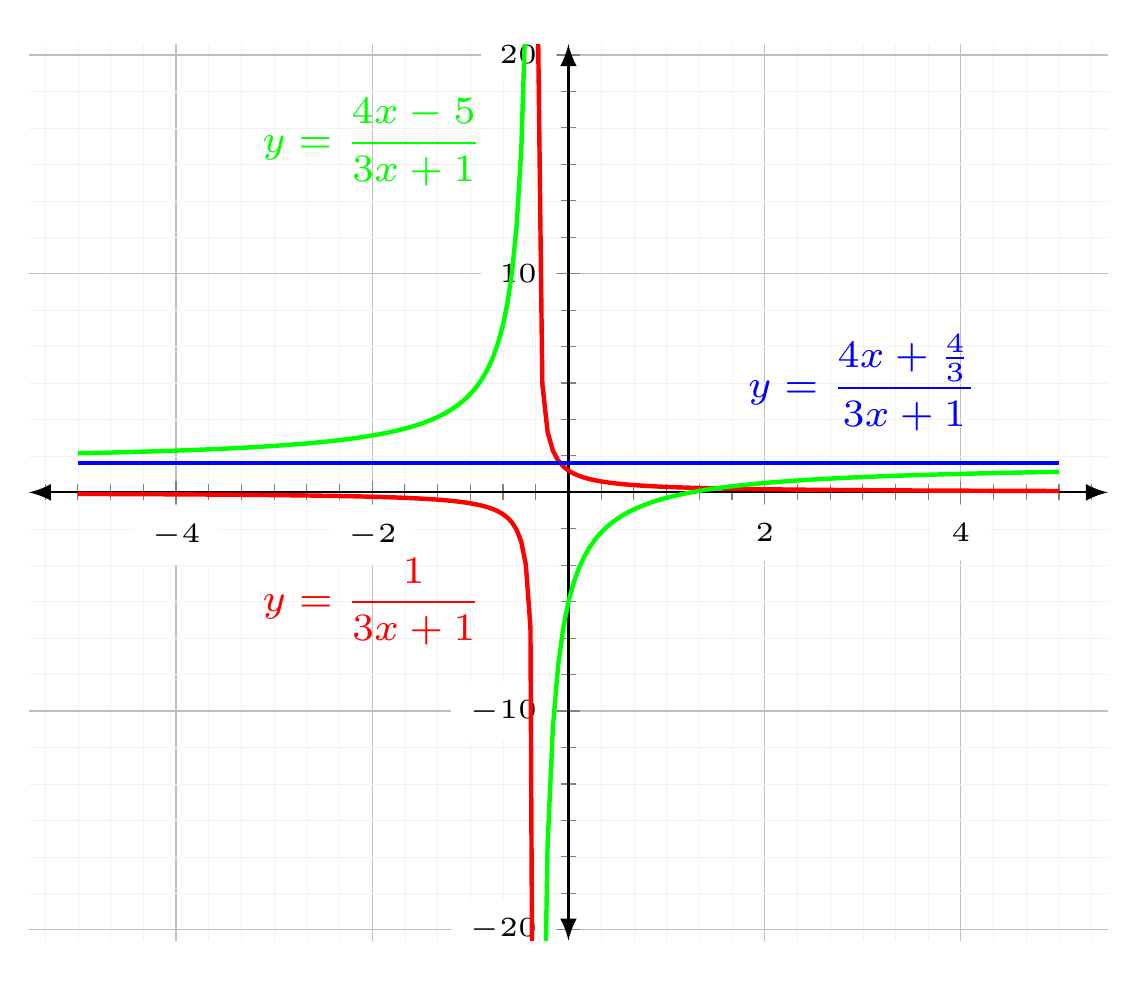
\begin{tikzpicture}[scale=2, declare function={f(\x)=1/(3*\x+1);}, declare function={g(\x)=(4*\x-5)/(3*\x+1);}]
		\begin{axis}[xmin=-5,xmax=5,
							 ymin=-20,ymax=20,
   							 grid=both,
    						 grid style={line width=.1pt, draw=gray!10},
    						 major grid style={line width=.2pt,draw=gray!50},
    						 axis lines=middle,
    						 minor tick num=5,
     						 enlargelimits={abs=0.5},
   							 axis line style={latex-latex},
   							 ticklabel style={font=\tiny,fill=white},
   							 xlabel style={at={(ticklabel* cs:1)},anchor=north west},
   							 ylabel style={at={(ticklabel* cs:1)},anchor=south west}]
		\addplot[mark=none, red, thick, samples=100, domain=-5:-0.34, range=-20:20]{f(x)} node at (axis cs:-2,-5) 
		{\scriptsize $y = \dfrac{1}{3x+1}$};
		\addplot[mark=none, red, thick, samples=100, domain=-0.32:5, range=-20:20]{f(x)} node at (axis cs:-2,-5){};
		\addplot[mark=none, green, thick, samples=100, domain=-5:-0.34, range=-20:20, unbounded coords=jump]{g(x)} node at (axis cs:-2,16) 
		{\scriptsize $y = \dfrac{4x-5}{3x+1}$};
		\addplot[mark=none, green, thick, samples=100, domain=-0.32:5, range=-20:20, unbounded coords=jump]{g(x)} node at (axis cs:2.5,16){};
		\addplot[mark=none, blue, thick, samples=50, domain=-5:5]{4/3} node at (axis cs:3,5) {\scriptsize $y = \dfrac{4x+\tfrac{4}{3}}{3x+1}$};
		\end{axis}
	\end{tikzpicture}
	\end{figure}
	
	\paragraph{}
	Each graph exhibits interesting properties. We can see the behavior of the red and green ones at the point $x = -\frac{1}{3}$. The blue one, 
	however, seems to be very different, even though the function is rational and has a non-zero denominator. Why is that so? Well this is because
	we can write:
	\[ \dfrac{4x+\tfrac{4}{3}}{3x+1} = \dfrac{4}{3} \cdot \dfrac{3x+1}{3x+1} \]
	
	\paragraph{}
	and we are free to cancel out the two $3x+1$ terms, provided $x \neq -\frac{1}{3}$. This somewhat explains the graph's behavior at every
	point; including the point $x = -\frac{1}{3}$ where it \textit{seems} to be defined. However, the function is still undefined at this point. 
	Moreover, this point is still a singularity of the function. We call this type of singularity a \textbf{removable singularity}. Singularities of this
	type, as the name suggests, can be ``removed'' by defining an appropriate value for them. In particular, the value to define must be done
	so that the function ``behaves well'' around that point. So if $f$ represented the blue function, we can write:
	\[ f(x) = \begin{cases} \frac{4x+\tfrac{4}{3}}{3x+1}, & x \neq -\frac{1}{3} \\ \frac{4}{3}, &  x = -\frac{1}{3} \end{cases} \]
	
	\paragraph{}
	You might be thinking ``wait, but couldn't we just cancel out the $3x+1$ term and just define the function as $f(x) = \frac{4}{3}$?''
	The answer is \textbf{yes}, we can do so, provided the situation allows for it. We must ask: ``can we \textbf{always} cancel such terms
	out without worry? Does every removable singularity come from a cancelable term?'' For the first question, the answer is \textbf{yes}. Given
	that there are two terms which can be canceled out, we are able to cancel them out and the resulting function will be nice(r) in the sense
	that the singularity will have been removed. But for the second question, try answering it yourself by graphing:
	\[ y = \dfrac{\e^{x-1} -1}{(x+1)(x-1)} \]
	
	\paragraph{}
	If you've answered \textbf{no} to the second question after graphing the above, come back to this question after finishing calculus.
	You may have noticed that I used the term ``behaves well'' when describing a removable singularity. This is for lack of a better term,
	which can't be used this early in the course. If you're interested, search up \textit{complex analysis}.
	
	\paragraph{}
	Now let's look at the red and green functions. There's nothing to cancel out in either of them. Let's first look at the red function,
	$f(x) = \frac{1}{3x+1}$. We notice its behavior at $x = -\frac{1}{3}$; it goes to infinity in two directions (negative infinity as $x$ 
	approaches it from the left and positive infinity from the right). Why is that so? Well we can make the observation that for $x < -\frac{1}{3}$,
	we have $f(x) < 0$; similarly for $x > \frac{1}{3}$, we have $f(x) > 0$. Moreover for $x$ near $-\frac{1}{3}$, we are essentially dividing
	1 by a term very close to zero, which yields either a very large positive value or a very ``large'' negative value (be careful here, because
	just saying a ``very small'' value may imply values near zero; here we mean values which are large when ignoring the sign). We call this 
	type of singularity a \textbf{pole}, and with it comes the line $x = -\frac{1}{3}$ which describes the line which the function is getting very 
	close to but never reaches. This line is called an \textbf{asymptote}; in particular, a \textbf{vertical asymptote} (because the line is vertical).
	
	\paragraph{}
	We can also observe that as $x$ approaches either positive or negative infinity, $f$ approaches zero. It's intuitive to see why this is the
	case; as we divide $1$ by (positively or negatively) larger values, the result will be very ``small'' in the sense that it's near zero.
	Here we have that as $x$ approaches either infinity, the function $f$ gets very close to the line $y=0$ (the $x$-axis) but never reaches it.
	We call this line a \textbf{horizontal asymptote}.
	
	\paragraph{}
	To mathematically state these facts about (what we call) \textit{asymptotic behavior}, we can write:
	\begin{multicols}{2}
	\begin{itemize}
		\item $\displaystyle \lim_{x \to -\frac{1}{3}^+} f(x) = +\infty$
		\item $\displaystyle \lim_{x \to -\frac{1}{3}^-} f(x) = -\infty$
		\item $\displaystyle \lim_{x \to +\infty} f(x) = 0$
		\item $\displaystyle \lim_{x \to -\infty} f(x) = 0$
	\end{itemize}
	\end{multicols}
	
	\paragraph{}
	This may take some explaining if you're not familiar with it (the \textbf{closed} interval $[-\infty, \infty]$ implies inclusion of 
	infinities themselves as well):\\
	
	\begin{kp}[Limit notation]
		If a real-valued function $f$ approaches a value $L_+ \in [-\infty, \infty]$
		as $x$ approaches a value $a \in [-\infty, \infty]$ from the right side (positive side) and $f$ approaches a value $L_- \in [-\infty, \infty]$
		as $x$ approaches $a$ from the left (negative side), then we write:
		\[ \lim_{x \to a^+} f(x) = L_+ \]
		\[ \lim_{x \to a^-} f(x) = L_- \]
		
		If $L_+ = L_-$, then we can set $L = L_+ = L_-$ and write:
		\[ \lim_{x \to a} f(x) = L \]
		
		Note that if $a = \pm \infty$, we can omit the superscript $+$ or $-$ from the limit, as infinity can only be approached from one side.
	\end{kp}
	
	\paragraph{}
	We will come back to this limit notation in calculus and use it quite a bit.
	Remember that the asymptote itself is the \textbf{line} which the function approaches, not the limit itself. We have:\\
	
	\begin{kp}[Asymptotes]
		If $f$ is a real-valued function, $a, L \in (-\infty, \infty)$ and either or both of the following hold:
		\begin{itemize}
			\item $\displaystyle \lim_{x \to \infty} f(x) = L$ or $\displaystyle \lim_{x \to -\infty} f(x) = L$
			\item $\displaystyle \lim_{x \to a^-} f(x) = \pm \infty$ or $\displaystyle \lim_{x \to a^+} f(x) = \pm \infty$
		\end{itemize}
		
		Then:
		\begin{itemize}
			\item $y = L$ is a \textbf{horizontal asymptote} of $f$
			\item $x = a$ is a \textbf{vertical asymptote} of $f$
		\end{itemize}
	\end{kp}
	
	\paragraph{}
	Observe that we need $a$ and $L$ to be non-infinity for this to work; the line defined by $y = \infty$, for example, doesn't really make sense.
	
	\paragraph{}
	Now, let's consider the green function, $g(x) = \frac{4x-5}{3x+1}$. This time, however, we shall determine the behavior and compute the 
	asymptotes without just looking at the graph (we'll still use the graph as reference though). How can we compute limits? Well, we have
	a way of getting \textit{vertical} asymptotes by finding singularities (particularly poles). Since no terms in $g$ can cancel out, we have
	a pole at $x = -\frac{1}{3}$ (which makes the denominator zero). Thus, our (only) vertical asymptote is the line $x = -\frac{1}{3}$.
	
	\paragraph{}
	As for the horizontal one, the graph shows that $g$ doesn't actually approach zero as $x \to \pm \infty$. It looks like it approaches the
	blue line, but how can we show this? We need only use the following (very intuitive) fact:\\
	
	\begin{pf}
		\begin{theorem*}
			If $n \geqslant 1$ and $k \in \R$, then $\displaystyle \lim_{x \to \pm \infty} \dfrac{k}{x^n} = 0$
		\end{theorem*}

		\tcbline		
		
		\begin{proof}
			This is clear when $k=0$, so we can assume $k \neq 0$. The proof below uses techniques which are beyond the scope 
			of IB, but written here for those who are interested.\\
			
			Let $\varepsilon > 0$ and choose $x_0 = \sqrt[n]{\frac{|k|}{\varepsilon}}$. Let $x \in \R$ satisfy $x >x_0$. Then:
			\[ |f(x) - 0| = |f(x)| = \left\vert \dfrac{|k|}{x^n} \right\vert = \dfrac{|k|}{|x|^n} < \dfrac{|k|}{|x_0|^n} = \dfrac{|k|}{\tfrac{|k|}
			{\varepsilon}} = \varepsilon \]
			
			Which proves that $\displaystyle \lim_{x \to +\infty} \frac{k}{x^n} = 0$. Analogously, choose $x_0 = -\sqrt[n]{\frac{|k|}{\varepsilon}}$,
			let $x \in \R$ satisfy $x < x_0$ and the exact same argument as above yields:
			\[ |f(x) - 0| < \varepsilon \]
			
			once again, which proves $\displaystyle \lim_{x \to -\infty} \frac{k}{x^n} = 0$.
		\end{proof}
	\end{pf}
	
	\paragraph{}
	This theorem gives us a tool to help use determine limits. Let's apply it to $g(x) = \frac{4x-5}{3x+1}$. First write:
	\[ g(x) = \dfrac{4x-5}{3x+1} = \dfrac{\tfrac{1}{x}}{\tfrac{1}{x}} \cdot \dfrac{4x-5}{3x+1} = \dfrac{4-\tfrac{5}{x}}{3+\tfrac{1}{x}} \]
	
	\paragraph{}
	We can do so because we are taking $x \to \pm \infty$, which is very far away from zero (thus we won't be dividing by zero in the limit
	calculation). Then:
	\[ \lim_{x \to \pm \infty} g(x) = \lim_{x \to \pm \infty} \dfrac{4-\tfrac{1}{x}}{3+\tfrac{1}{x}} = \dfrac{4-0}{3+0} = \dfrac{4}{3} \]
	
	\paragraph{}
	This means our horizontal asymptote is $y = \frac{4}{3}$, which is exactly the equation of the blue line. You may have noticed that
	even though we used the statement in the theorem, how do we know we can apply it the way we did? How do we know that the limit
	of a quotient is the quotient of limits? We didn't prove anything about how we can use the limit operation; we can for sure and we will,
	but doing so now would be a huge digression from the topic at hand. We shall wait for the calculus topic and prove all limit rules there.
	
	\paragraph{}
	
		
\newpage
	
\section{Appendix A}

	\paragraph{}
	Below are the proofs of some additional theorems which were left out of the main body either for the sake of brevity or because they
	went off-topic.\\

	\begin{pf}
		\label{apA:ctble-union}
		\begin{theorem*}
			Let $U_1, U_2, ..., U_n, U_{n+1}, ...$ be a countable collection of countable sets. Then the set $U = \bigcup_{i \in \N} U_i$
			is countable.
		\end{theorem*}

		\tcbline		
		
		\begin{proof}
			Since each $U_k$ ($k \in \Z^+$) is countable, there is a bijection $\phi_k : U_k \to \N$. Let $\psi : U \to \N \times \N$ be defined
			by $\phi(x) = (m_x, \phi_{m_x})$ where $m_x \in \Z^+$ is the least value such that $x \in U_{m_x}$. We observe that for 
			$x,y \in U$, 
			$\psi(x) = \psi(y) \iff (m_x, \phi_{m_x}) = (m_y, \phi_{m_y}) \iff m_x = m_y \text{ and } \phi_{m_x} = \phi_{m_y} \iff m_x = m_y$.
			Thus, $\psi$ is injective.\\
			
			Now let $\omega : \N \times \N \to \N$ be defined by $\omega(a,b) = 2^a(2b-1)$. We observe that $\omega(a,b) = \omega(c,d)
			\iff 2^a(2b-1) = 2^c(2d-1)$. If $a = b$, then $2b-1 = 2d-1 \iff b = d$ and we're done. Otherwise suppose $a<c$. Then
			$2b-1 = 2^{c-a}(2d-1)$. The LHS is odd while the RHS is even, which is a contradiction. We thus conclude that $a=c$ is required,
			which proves $\omega$ is injective.\\
			
			Finally, we have that $\omega \circ \psi : U \to \N$ is injective, which proves $U$ is countable (either finite or countably-infinite).
		\end{proof}
	\end{pf}
	
	\hfill
	
	\begin{pf}
		\label{apA:fta}
		\begin{theorem*}
			Fundamental Theorem of Arithmetic:\\
			For all $n \in \N$ with $n > 1$, $n$ can be written \textbf{uniquely} as a product of prime numbers.
		\end{theorem*}

		\tcbline		
		
		\begin{proof}
			We proceed by strong induction. The base case is $n=2$, which is clearly true because 2 is prime.
			Suppose the theorem holds for all $n < k$ for some $k > 1$. If $k$ is prime, we're done. Otherwise, suppose $k$ is not
			prime. Then $k$ can be written as a product of two integers $a$ and $b$ with $2 \leqslant a, b < k$.
			That is, $k = ab$. Now $a,b < k$ means the inductive hypothesis holds for $a$ and $b$. So we can write
			$a$ and $b$ as a product of primes, which means $k = ab$ is also a product of primes. This means the theorem
			holds for $k$, thus proving that every integer $n > 1$ can be written as a product of primes.\\
			
			For uniqueness, suppose $a = p_1 p_2 \cdots p_m = q_1 q_2 \cdots q_n$ where $p_1, ..., p_m, q_1, ..., q_n$
			are primes. Then $p_1$ divides $a$, which means it divides one of $q_1, ..., q_n$ as well. Since they are prime, we must
			have that $p_1 = q_i$ for some $i$. WLOG, suppose $i = 1$ so $p_1 = q_1$. Then we have that
			$p_2 p_3 \cdots p_m = q_2 q_3 \cdots q_n$. Repeating this process, suppose (WLOG) that $m > n$. Then we get that
			$p_{n+1} p_{n+2} \cdots p_m = 1$. But this isn't possible, since 1 can't be written as a product of primes. Therefore, we
			need $m=n$ and consequently $p_i = q_i$ for each $i \in \{1, ..., m=n\}$. This proves uniqueness.
		\end{proof}
	\end{pf}
	
	\hfill
	
	\begin{pf}
		\label{apA:q-count-fta}
		\begin{theorem*}
			$\Q$ is countable (alternative proof using the Fundamental Theorem of Arithmetic)
		\end{theorem*}

		\tcbline		
		
		\begin{proof}
			We take a bijection $f : \N \to \Z$ satisfying $f(0) = 0$ (it's been shown that $\Z$ is countable on page \pageref*{pf:z-count}).
			We wish to find a bijection $g : \Z \to \Q$. By the Fundamental Theorem of Arithmetic, we know that every positive
			integer in $\Z^+$ can be written either as 1 or a product of primes ${p_1}^{r_1} {p_2}^{r_2} \cdots {p_k}^{r_k}$ (with $p_1, ..., p_k$ 
			distinct primes and non-negative powers $r_1, ..., r_k$).\\
			
			We can extend this to the positive rational numbers. Every $\frac{m}{n} \in \Q^+$ (with $m,n \in \Z^+$) can be
			written as either $1$ or a quotient of a product of primes $\frac{{p_1}^{r_1} {p_2}^{r_2} \cdots {p_k}^{r_k}}
			{{q_1}^{s_1} {q_2}^{s_2} \cdots {q_l}^{s_l}} = {p_1}^{r_1} {p_2}^{r_2} \cdots {p_k}^{r_k} {q_1}^{-s_1} {q_2}^{-s_2} \cdots {q_l}^{-s_l}$. 
			WLOG, we can
			assume $\gcd(m,n) = 1$ and we have that $p_i \neq q_j$ for any $i = 1, ..., r$ and $j = 1, ..., s$ (otherwise, we may cancel them out).
			Observe that this gives a unique prime factorization for each $q \in \Q^+$, where we include negative powers as well; and
			by setting all powers to zero, we would get 1.\\
			
			Now define a function $h : \Z^+ \to \Q^+$ by:
			\[ h(m) = h({p_1}^{r_1} {p_2}^{r_2} \cdots {p_k}^{r_k}) = {p_1}^{f(r_1)}{p_2}^{f(r_2)} \cdots {p_k}^{f(r_k)} \]
			
			This function is \textbf{injective} because if ${p_1}^{f(r_1)}{p_2}^{f(r_2)} \cdots {p_k}^{f(r_k)} = {q_1}^{f(s_1)}{q_2}^{f(s_2)} \cdots 
			{q_l}^{f(s_l)}$, uniqueness of the prime factorization and injectivity of $f$ tell us that we require $k=l$ and (WLOG) 
			${p_i}^{f(r_i)} = {q_i}^{f(s_i)} \implies p_i = q_i \text{ and } r_i = s_i$ for all $i = 1, ..., k$. Thus, we get that 
			${p_1}^{r_1} {p_2}^{r_2} \cdots {p_k}^{r_k} = {q_1}^{s_1} {q_2}^{s_2} \cdots {q_l}^{s_l}$.\\
			
			This function is also \textbf{surjective}. For each $q \in \Q^+$, we can write down $q = {p_1}^{r_1} {p_2}^{r_2} \cdots {p_k}^{r_k}$
			for $p_1, ..., p_k$ primes and $r_1, ..., r_k \in \Z$. Since $f$ is surjective, we can find $n_i \in \N$ for which $f(n_i) = r_i$ for each
			$i = 1, ..., k$. If $r_1 = r_2 = ... = r_k = 0$, we have $q = 1$ and $n_1 = n_2 = ... = 0$ (by how we chose $f$). We then see that
			$h(1) = 1$. Otherwise, suppose $r_1, ..., r_k \neq 0$ (zero-powers can be ignored because their values will end up being 1 anyway).
			Then we can find $n_i \in \Z^+$ for all $i = 1, ..., n$ such that $f(n_i) = r_i$ by surjectivity of $f$, and we have that:
			\[ q = {p_1}^{f(n_1)}{p_2}^{f(n_2)} \cdots {p_k}^{f(n_k)} \]
			
			Thus we can set $m = {p_1}^{n_1} {p_2}^{n_2} \cdots {p_k}^{n_k}$ to give $h(m) = q$, which proves $h$ is indeed surjective.\\
			
			We've therefore constructed a bijection $h : \Z^+ \to \Q^+$. Now write:
			\[ g(m) = \begin{cases} h(m), & m \in \Z^+ \\ -h(-m), & m \in \Z^- \\ 0, & m = 0 \end{cases} \]
			
			\paragraph{}
			It's clear that $g : \Z \to \Q$ is a bijection, which proves $\Q$ is countable.
		\end{proof}
	\end{pf}
	
	\hfill
	
	\begin{pf}
		\label{apA:r-uncount}
		\begin{theorem*}
			$\R$ is uncountable.
		\end{theorem*}

		\tcbline		
		
		\begin{proof}
			We need only prove a subset of $\R$ is uncountable. Let $B \subseteq \R$ be the subset of $\R$ defined by:
			\[ B = \{ 0.b_1b_2b_3... \; \vert \; b_i \in \{0,1\} \text{ for } i \in \Z^+  \} \]
			
			Suppose $B$ \textbf{is countable}. Then we can write \textbf{all} elements $\beta_1, \beta_2, \beta_3, ... \in B$ as:
			\[ \beta_1 = 0.b_{11}b_{12}b_{13}... \]
			\[ \beta_2 = 0.b_{21}b_{22}b_{23}... \]
			\[ \beta_3 = 0.b_{31}b_{32}b_{33}... \]
			\[ \vdots \]
			
			for $b_{i,j} \in \{0, 1\}$. Now construct a number $\beta = 0.\overline{b_{11}} \, \overline{b_{22}} \, \overline{b_{33}}...$
			where $\overline{b_{ii}} = 1$ if $b_{ii} = 0$ and $\overline{b_{ii}} = 0$ if $b_{ii} = 1$. It's clear that $\beta \in B$ but apparent
			that $\beta \neq \beta_k$ for any $k \in \Z^+$ by construction (since $\overline{b_{kk}} \neq b_{kk}$). Hence, we have
			that $\beta_1, \beta_2, \beta_3, ...$ isn't the entire set $B$, which proves $B$ must be uncountable.\\
			
			Since $B \subseteq \R$, it follows that $\R$ is uncountable as well.
		\end{proof}
	\end{pf}
	
	\hfill	
	
	\begin{pf}
		\label{apA:euc-div}
		\begin{theorem*}
			Euclidean Division Theorem for Polynomials:\\
			Given two non-zero polynomials $f(x)$ and $g(x)$ with $\deg(f) \geqslant \deg(g)$, there are polynomials
			$q(x)$ and $r(x)$ with $\deg(r) < \deg(g)$ or $r(x) = 0$ such that $f(x) = g(x)q(x) + r(x)$.
		\end{theorem*}

		\tcbline		
		
		\begin{proof}
			Write $f(x) = \sum_{k=0}^m a_k x^k$ and $g(x) = \sum_{k=0}^n b_k x^k$ for $a_m, b_n \neq 0$ and $m \geqslant n$.
			Let $d_1(x) = \frac{a_m}{b_n}x^{m-n}$ and let $h_1(x) = f(x) - d_1(x) g(x)$.
			Observe that either $h_1(x) = 0$ or $\deg(h_1) < \deg(f)$, which is clear by construction.
			If $h_1(x) = 0$, we can set $r(x) = 0$ and $q(x) = d_1(x)$ to give $f(x) = q(x) g(x) + r(x)$, as desired.\\
			
			Otherwise, we have $\deg(h_1) < \deg(f)$. If $\deg(h_1) < \deg(g)$, we
			can write $q(x) = d_1(x)$ and $r(x) = h_1(x)$ to give $f(x) = q(x) g(x) + r(x)$ as desired. If $\deg(h_1) \geqslant \deg(g)$, repeat the 
			process with $d_2(x)$ chosen such that $h_2(x) = h_1(x) - d_2(x) g(x)$ and either $h_2(x) = 0$ or $\deg(h_2) < \deg(h_1)$.\\
			
			By repeating this process further, we
			eventually we reach a point where either $h_k(x) = 0$ or $\deg(h_k) < \deg(g)$ for some $k$ and we have $h_k(x) = h_{k-1}(x) - 
			d_k(x) g(x) = f(x) - g(x) [d_1(x) + ... + d_k(x)]$.
			We can set $q(x) = d_1(x) + ... + d_k(x)$ and $r(x) = h_k(x)$ to give $f(x) = q(x) g(x) + r(x)$ as desired.
		\end{proof}
	\end{pf}
	
	\newpage	
	
\section{Bibliography}
	\begin{itemize}
		\item Herstein, I.N. (1964), Topics in Algebra, Ginn and Company, ISBN 0-471-02371-X
		\item Remmert, Reinhold (1991), "What is $\pi$?", Numbers, Springer, p. 129
		\item Arndt, Jörg; Haenel, Christoph (2006). Pi Unleashed. Springer-Verlag. ISBN 978-3-540-66572-4. Retrieved 5 June 2013. 
		English translation by Catriona and David Lischka.
		\item Posamentier, Alfred S.; Lehmann, Ingmar (2004). Pi: A Biography of the World's Most Mysterious Number. Prometheus Books. 
		ISBN 978-1-59102-200-8.
		\item \sloppy \url{https://upload.wikimedia.org/wikipedia/commons/c/cb/Epsilonschlauch.svg}
	\end{itemize}		
\end{document}




